\newcommand{\CLASSINPUTinnersidemargin}{0.7in}
\newcommand{\CLASSINPUToutersidemargin}{0.7in}
\documentclass{article}

\usepackage{fullpage} % use entire page layout
\usepackage{times}     % smaller and better fonts that the standard latex ones
\usepackage[letterpaper]{geometry} % force letter format
\usepackage[colorlinks=true,linkcolor=black,urlcolor=blue,anchorcolor=black,citecolor=black,backref=none]{hyperref}
\usepackage[usenames,dvipsnames]{color}
%% Disable backref and make \href colors more decent:
\definecolor{MyDarkBlue}{rgb}{0,0.1,0.7}
\hypersetup{pdfborder={0 0 0},colorlinks,breaklinks=true,
  urlcolor={MyDarkBlue},citecolor={MyDarkBlue},linkcolor={MyDarkBlue} }
\newcommand{\ebookurl}{http://www.sigcomm.org/content/ebook}

% Package to generate and customize Algorithm as per ACM style
\usepackage[ruled]{algorithm2e}
\renewcommand{\algorithmcfname}{ALGORITHM}
\SetAlFnt{\small}
\SetAlCapFnt{\small}
\SetAlCapNameFnt{\small}
\SetAlCapHSkip{0pt}
% \IncMargin{-\parindent}

\usepackage{amsmath, amssymb, epsfig, graphicx, psfrag}
\usepackage{multirow}
\usepackage{sidecap}
\usepackage{caption,cleveref,subcaption}
\usepackage{array}
\usepackage{colortbl}
\usepackage{url}
\usepackage{cite}
%\usepackage{fullpage}
\usepackage{enumerate}
 
\def\del{\partial}
\def\ds{\displaystyle}
\def\ts{\textstyle}
\def\beq{\begin{equation}}
\def\eeq{\end{equation}}
\def\beqa{\begin{eqnarray}}
\def\eeqa{\end{eqnarray}}
\def\beqan{\begin{eqnarray*}}
\def\eeqan{\end{eqnarray*}}
\def\nn{\nonumber}
\def\binomial{\mathop{\mathrm{binomial}}}
\def\half{{\ts\frac{1}{2}}}
\def\Half{{\frac{1}{2}}}
\def\N{{\mathbb{N}}}
\def\Z{{\mathbb{Z}}}
\def\Q{{\mathbb{Q}}}
\def\R{{\mathbb{R}}}
\def\C{{\mathbb{C}}}
\def\argmin{\mathop{\mathrm{arg\,min}}}
\def\argmax{\mathop{\mathrm{arg\,max}}}
 \def\diag{\mathop{\mathrm{diag}}}
\def\x{\times}
\def\limn{\lim_{n \rightarrow \infty}}
\def\liminfn{\liminf_{n \rightarrow \infty}}
\def\limsupn{\limsup_{n \rightarrow \infty}}
\def\GV{Guo and Verd{\'u}}

%\newtheorem{proposition}{Proposition}
%\newtheorem{definition}{Definition}
%\newtheorem{theorem}{Theorem}
%\newtheorem{lemma}{Lemma}
%\newtheorem{corollary}{Corollary}
%\newtheorem{assumption}{Assumption}
%\newtheorem{algorithm}{Algorithm}
%\newtheorem{claim}{Claim}
\def\qed{\mbox{} \hfill $\Box$}
%\setlength{\unitlength}{1mm}

\newtheorem{thm}{Proposition}  

\def\ehat{\widehat{e}}
\def\qhat{\widehat{q}}
\def\rhat{\widehat{r}}
\def\uhat{\widehat{u}}
\def\xhat{\widehat{x}}
\def\zhat{\widehat{z}}
\def\la{\leftarrow}
\def\ra{\rightarrow}
\def\SR{\mbox{\small \sffamily SR}}
\def\SRTX{\mbox{\small \sffamily SRTX}}
\def\SRRX{\mbox{\small \sffamily SRRX}}
\def\MRX{\mbox{\small \sffamily MRX}}
\def\SNR{\mbox{\small \sffamily SNR}}
\def\SINR{\mbox{\small \sffamily SINR}}
\def\arr{\rightarrow}
\def\Exp{\mathbf{E}}
\def\var{\mbox{\bf var}}

\def\Xset{{\cal X}}

\newcommand{\one}{\mathbf{1}}
\newcommand{\abf}{\mathbf{a}}
\newcommand{\bbf}{\mathbf{b}}
\newcommand{\dbf}{\mathbf{d}}
\newcommand{\ebf}{\mathbf{e}}
\newcommand{\gbf}{\mathbf{g}}
\newcommand{\hbf}{\mathbf{h}}
\newcommand{\pbf}{\mathbf{p}}
\newcommand{\qbf}{\mathbf{q}}
\newcommand{\qbfhat}{\widehat{\mathbf{q}}}
\newcommand{\rbf}{\mathbf{r}}
\newcommand{\sbf}{\mathbf{s}}
\newcommand{\sbfhat}{\widehat{\mathbf{s}}}
\newcommand{\tbf}{\mathbf{t}}
\newcommand{\ubf}{\mathbf{u}}
\newcommand{\utildebf}{\tilde{\mathbf{u}}}
\newcommand{\vbf}{\mathbf{v}}
\newcommand{\wbf}{\mathbf{w}}
\newcommand{\xbf}{\mathbf{x}}
\newcommand{\xbfhat}{\widehat{\mathbf{x}}}
\newcommand{\ybf}{\mathbf{y}}
\newcommand{\zbf}{\mathbf{z}}
\newcommand{\zbfhat}{\widehat{\mathbf{z}}}
\newcommand{\Abf}{\mathbf{A}}
\newcommand{\Bbf}{\mathbf{B}}
\newcommand{\Dbf}{\mathbf{D}}
\newcommand{\Gbf}{\mathbf{G}}
\newcommand{\Pbf}{\mathbf{P}}
\newcommand{\Qbf}{\mathbf{Q}}
\newcommand{\Sbf}{\mathbf{S}}
\newcommand{\Ubf}{\mathbf{U}}
\newcommand{\Wbf}{\mathbf{W}}
\newcommand{\Xhat}{\widehat{X}}
\newcommand{\Xbf}{\mathbf{X}}
\newcommand{\Ybf}{\mathbf{Y}}
\newcommand{\Zbf}{\mathbf{Z}}
\newcommand{\Zhat}{\widehat{Z}}
\newcommand{\Zbfhat}{\widehat{\mathbf{Z}}}
\newcommand{\thetabf}{{\bm{\theta}}}
\newcommand{\mubf}{{\bm{\mu}}}
\newcommand{\mubar}{\overline{\mu}}
\newcommand{\muavg}{\mu}
\newcommand{\sigbf}{\bm{\sigma}}
\newcommand{\etal}{\emph{et al.}}
\newcommand{\eg}{\emph{eg.}}

\def\Nrx{N_{\rm rx}}
\def\Ntx{N_{\rm tx}}

%\usepackage[compact]{titlesec}

%\input{journal_names.tex}

%\def\negSpace{\hspace{-0.15in}}
%%\oddsidemargin -0.15in \evensidemargin -0.15in
%\oddsidemargin 0in \evensidemargin 0in
%\marginparwidth 40pt \marginparsep 10pt
%\topmargin 0pt \headsep 0in
%\textheight 8.85in \textwidth 6.5in
\title{Smart Data Pricing (SDP): \\ Economic Solutions to Network Congestion}
\author{Soumya Sen\footnote{Present affiliation: University of Minnesota}, Carlee Joe-Wong, Sangtae Ha\footnote{Present affiliation: DataMi}, Mung Chiang\\Princeton University}
\date{}
\begin{document}



\maketitle

%\begin{abstract}
%The unprecedented growth in demand for data is causing serious concerns about the technological sustainability and economic viability of the Internet. Traditionally, network operators have used simple flat-rate broadband data plans for both wired and wireless network access. But today, with the popularity of mobile devices and exponential growth of apps, videos, and clouds, service providers are gradually moving towards more sophisticated pricing schemes, including dynamic pricing. This decade will therefore likely witness a major change in ways in which network resources are managed and the role of economics in allocating these resources.  Students in Computer Science and Electrical Engineering therefore need to be equipped with an adequate knowledge about the interplay between technological and economic factors in making prudent design choices for networked systems. In particular, they need to have a good overview of economic concepts, network pricing models, system design, pricing signaling mechanisms and protocols, and the impact of human factors on pricing decisions. Unfortunately, most of these materials are not readily available as a single source for quick reference; they are scattered across published articles, white papers, news reports, and industry technical reports, from across researchers in diverse fields. It is therefore important for the networking community to create a chapter that organizes the relevant materials in a holistic approach, drawing on both past and present literature in engineering and economics, theory and systems, academia and industry. This proposed chapter will review some of the well-known past broadband pricing proposals (both static and dynamic) and their current realizations in various consumer data plans around the world, discuss several research challenges and developments, and provide an in-depth analysis of economic models and systems design for smart dynamic pricing. It will also provide a brief overview of the relationships between various pricing ideas in broadband data plans and their counterparts in other markets, such as electricity and transportation networks.  By exploring the economics of Internet data pricing, this work attempts to facilitate the academic community's efforts in understanding the existing literature, recognizing new trends, and shaping an appropriate and timely research agenda.  Graduate students will also benefit from a discussion of the open questions and challenges in pricing for identifying project and research topics, as well as access to video lectures, slides, class notes, and exercise questions to help them better understand the material.
%\end{abstract}

%\noindent
% {\bf Keywords --} Economic aspects of the Internet, Network economics, Broadband pricing\\

\section{Introduction}\label{intro}

Advances in Internet technologies have resulted in an unprecedented growth in demand for data. In particular, demand in the mobile Internet sector is doubling every year \cite{CiscoVNI}. Given the limited wireless spectrum availability, the rate of growth in the supply of wireless capacity (per dollar of investment) is unlikely to match the rate of growth in demand in the long run. Internet Service Providers (ISPs) are therefore turning to new pricing and penalty schemes in an effort to manage the demand on their network, while also matching their prices to cost. But changes in pricing and accounting mechanisms, if not done carefully, can have significant consequences for the entire network ecosystem. Multiple stakeholders in this ecosystem, including operators, consumers, regulators, content providers, hardware and software developers, and architects of network technologies, have all been tackling these issues of charging and allocating limited network resources. Even back in 1974, while writing about the future challenges of computer communication networks, Leonard Kleinrock \cite{Kleinrock} noted: 
\begin{quote}
\emph{[H]ow does one introduce an equitable charging and accounting scheme in such a mixed network system? In fact, the general question of accounting, privacy, security and resource control and allocation are really unsolved questions which require a sophisticated set of tools.}
\end{quote}
While much progress has been made on developing technical solutions, methods, and tools to address these issues, continued growth of the network ecosystem requires developing a better understanding of the underlying economic and policy perspectives. The broader area of \emph{network economics}, which deals with the interplay between technological and economic factors of networks, is therefore receiving more attention from engineers and researchers today. Economic factors like pricing, costs, incentive mechanisms and externalities\footnote{Network externality is the notion that the cost or value of being a part of a network for an individual user depends on the number of other users using that network. For example, the value of a network grows as more users adopt and positive externalities are realized from being able to communicate with other users on the network. Similarly, when many users start to content for limited resources of a bottleneck link of a network, negative externalities from congestion diminish a user's utility from accessing the network.} affect the  adoption outcomes (i.e., success or failure of network technologies) and stability \cite{Sen2010,Joseph2007,wifi-3g-infocom}, influence network design choices \cite{Sen2011-MVF,Sen2009-SVS}, and impact service innovation \cite{Zhang2010}. Conversely, technological limitations and regulatory constraints determine which kind of economic models are most suited to analyze a particular network scenario. This interplay between technology, economics, and regulatory issues is perhaps most easily observed in the case of broadband access pricing, for example, in evaluating the merits of ``flat-rate" versus ``usage-based" pricing or the neutrality of ``volume-based" versus ``app-based" accounting, etc. In this chapter we discuss the current trends in access pricing among service operators, factors that affect these decisions, analytical models and related considerations. In particular, we observe that \emph{Smart Data Pricing}\footnote{SDP is the broad set of ideas and principles that goes beyond the traditional flat-rate or byte-counting models and instead considers pricing as a network management solution. See http://www.smartdatapricing.org.} (SDP) is likely to emerge as an effective way to cope with increased network congestion. These smarter ways to count and treat data traffic illustrate three shifts in the principles of network management:

\begin{enumerate}
\item {\bf \emph{Pricing for end-user Quality of experience (QoE) and not just byte-counting}}: Simple policies like usage-based pricing (byte-counting) (a) force users to pay the same amount per unit of bandwidth consumed irrespective of the congestion levels on the network,\footnote{In 1997, David Clark wrote \cite{DDClark} that ``The fundamental problem with simple usage fees is that they impose usage costs on users regardless of whether the network is congested or not."} and (b) fail to account for the fact that different applications have different bandwidth requirements to attain a certain QoE for the user. SDP should try to match the cost of delivering application-specific desired QoE requirements of the user to the ISP's congestion cost at the time of delivery.     
\item {\bf \emph{Application layer control to impact physical layer resource management}}:  Today's smart devices with their easy to use graphical user interfaces can potentially enable consumer-specified choice for access quality. Whether done manually or in an automated mode, users' specifications of their willingness to pay for their desired QoE of different applications can be taken in as inputs at the APP layer and used to control PHY layer resource allocation and media selection (e.g., WiFi offloading versus 3G). But enabling this requires consumer trials to understand how to design incentives and create interfaces that can be effective in modifying end-user behavior.
\item {\bf \emph{Incorporating edge devices as a part of network management system}}: Instead of managing traffic only in the network core, SDP explores ways to make edge devices (e.g., smart mobile devices and customer-premise equipments like gateways) a part of the network resource allocation and management system. For example, instead of throttling traffic in the network core using the policy charging and rules function (PCRF), the edge devices (e.g., home gateways) themselves could locally regulate demand based on a user's budget, QoE requirements, and network load or available prices. Such measures to push control from the network core out to the end-users, while preserving the end-to-end principles of the Internet, have been gaining attention among networking research groups \cite{M3I}. 
\end{enumerate}

But before delving deeper into pricing ideas, let us pause to address some common misconceptions often encountered in public discourse. First, many believe that the Internet's development cost was borne by the United States Government, and hence that taxpayers have already paid for it. In reality, by 1994 the National Science Foundation supported less than 10\% of the Internet and by 1996 huge commercial investments were being made worldwide \cite{MIT}. 

Second, users often do not realize that the Internet is not free \cite{MIT, chetty2011my} and think its cost structure is the same as that of information goods. In contrast to \emph{information goods}, which tend to have zero marginal costs,\footnote{Marginal cost is the change in the total cost that arises when the quantity produced changes by one unit, e.g., the cost of adding one more unit of bandwidth.} Internet operators incur considerable network management operation and billing costs. MacKie-Mason and Varian \cite{MM-Varian} have shown that while the marginal cost of some Internet traffic can be zero because of \emph{statistical multiplexing}, congestion costs can be quite significant. 
In regard to delivery of bits, it is worthwhile to note that there are some important factors at play: 
\begin{enumerate}[(a)]
\item There is a large and growing variance in the QoE requirements of the different types of applications that consumers are using today, and
\item The network operator's cost of delivery per bit for a given QoE level also has significant variance, ranging from essentially zero marginal cost in uncongested times to very high in congested times.
\item There is also a variance in user's willingness to pay for different types of traffic and QoE levels.
\end{enumerate}

So why not match the right pairs? Most SDP ideas aim to do exactly that, i.e., match the operator's cost of delivering bits to the consumer's QoE needs for different application types at the amount they are willing to spend.

Third, there is a popular misconception that network costs are high because billing costs account for 50\% of telephony costs. Although true for running costs, it is only 4-6\% when depreciation of sunk costs is added \cite{M3I}. Another important cost for wireless operators today is the cost of acquiring new spectrum to support the growing bandwidth needs of the customers. However, spectrum is limited and expensive, and even auction-based spectrum reallocation schemes are projected to fall short of the demand for spectrum. 

Fourth, the belief that better technologies like 4G and offloading mechanisms will solve the problems is already being questioned -- ``The reasons are two-fold: The amount of spectrum made available to U.S. wireless companies is limited, but the carriers have also been sluggish in buying up enough backhaul to support their capacity requirements. There is only so much data that can be crammed into wireless spectrum -- and only so much spectrum available to wireless networks. Thanks to rising mobile data demands, a current wireless spectrum surplus of 225 MHz will become a deficit of 275 MHz by 2014, according to the FCC \cite{CNN-4G}."

%Higher access speeds lead to both higher demand and applications that consume higher amount of bandwidth. 

Fifth, users fear that changes in pricing policy will increase their access fees. This need not always be the case, as one can design incentive mechanisms that reward good behavior (e.g., price discounts in off-peak hours to incentivize shifting of usage demand from peak times). In other words, smarter pricing mechanisms can \emph{increase consumer choices} by empowering users to take better control of how they spend their monthly budget. For example, under time-dependent usage-based pricing \cite{comm-mag,ha2012tube}, users have better control over their monthly bills by choosing not only \emph{how much} they want to consume, but also \emph{when} they do so). Smart data pricing also has to be smart in its implementation and in its user interface design, with careful study of user psychology and human-computer interaction aspects, as we will illustrate in later sections and case studies. 

Lastly, we also need to remember that pricing is related to the market competition and user population density. For the interested reader, an overview of access fees in different parts of the world is provided in Section \ref{Dataplans}.

The following questions provide a useful way to think about SDP: 
\begin{enumerate}[(I)]
\item Why do we need SDP? Isn't network pricing an untouchable legacy?\\
Section \ref{sec:factors} provides an overview of the driving factors behind network congestion, and the challenges that it poses to various stakeholders of the network ecosystem are discussed in Section \ref{sec:threats}. We also discuss the rapid evolution in pricing among network operators and highlight in Section \ref{SDP} how Smart Data Pricing ideas will be useful in finding solutions that can work in today's networks.
\item Haven't other fields already used pricing innovations? What are the key SDP ideas relevant to communication networks?\\
We provide an overview of Internet pricing ideas in the existing literature in Section \ref{sec:congestion}, including some pricing plans from the electricity and transportation industries that can be applied to broadband pricing. Section \ref{sec:econ} provides an overview of a few examples and analytical models of known pricing mechanisms to illustrate key economic concepts relevant to the SDP literature. We also highlight many crucial differences between SDP in communication or data networks and pricing innovations in other industries.
\item Isn't SDP too complex to implement in the real world?\\
Section \ref{sec:TDP} provides a case study of a field trial of ``day-ahead time-dependent pricing" and discusses the model, system design, and user interface design considerations for realizing this plan. It serves to demonstrate both the feasibility of creating such SDP plans for real deployment while also pointing out the design issues that should be kept in mind. The discussion highlights the end-to-end nature of an SDP deployment, which requires developing pricing algorithms, understanding user psychology, designing an effective interface for communicating those prices to users, and implementing an effective system to communicate between the users and ISPs.
\item What are the outstanding problems in enabling SDP for the Internet?\\
SDP is an active area of research in the network economics community and a set of 20 questions and future directions are provided in Section \ref{sec:20Q} for researchers and graduate students to explore. Many of these research questions have been discussed at various industry-academia forums and workshops on SDP \cite{SDPForum,SDP2013}.  
\end{enumerate}


%This chapter is organized as follows: We first provide an overview of the driving factors behind network congestion in Section \ref{sec:factors} and discuss in Section \ref{sec:threats}, the various congestion related issues in the network ecosystem. We then discuss Smart Data Pricing principles and ideas in Section \ref{SDP}. An overview of pricing ideas in the existing literature is given in Section \ref{sec:congestion}, including some pricing plans from the electricity and transportation industries that can be applied to broadband pricing. Section \ref{sec:econ} provides an overview of a few examples and analytical models of known pricing mechanisms to illustrate key economic concepts essential for understanding the SDP literature. We then delve into one such pricing plan in Section \ref{sec:TDP}, namely, ``day-ahead time-dependent pricing,'' in order to illustrate the end-to-end nature of an SDP deployment, which requires developing pricing algorithms, designing an effective interface for communicating those prices to users, and implementing an effective system to communicate between an ISP and its users. Finally, in Section \ref{sec:20Q} we point to some (of many) research questions for broadband access pricing that are still open for further research in this area.



\section{Driving Factors of Network Congestion}\label{sec:factors}

With mobile devices becoming smarter, smaller, and ubiquitous, consumers are embracing the technology and driving up the demand for mobile data.  According to Cisco's VNI \cite{CiscoVNImobile}, in 2012, global mobile data traffic grew more than 70 percent year over year, to 855 petabytes a month. The growth rate varied by regions, with 44\% growth in Western Europe, and about 101\% in the Middle East and Africa and a 95\% growth rate in Asia Pacific. This section identifies some of the key factors that are expected to drive this growth in demand for mobile data (ref. Figure \ref{fig:driving_factors}).

\begin{figure}[h]
\centering
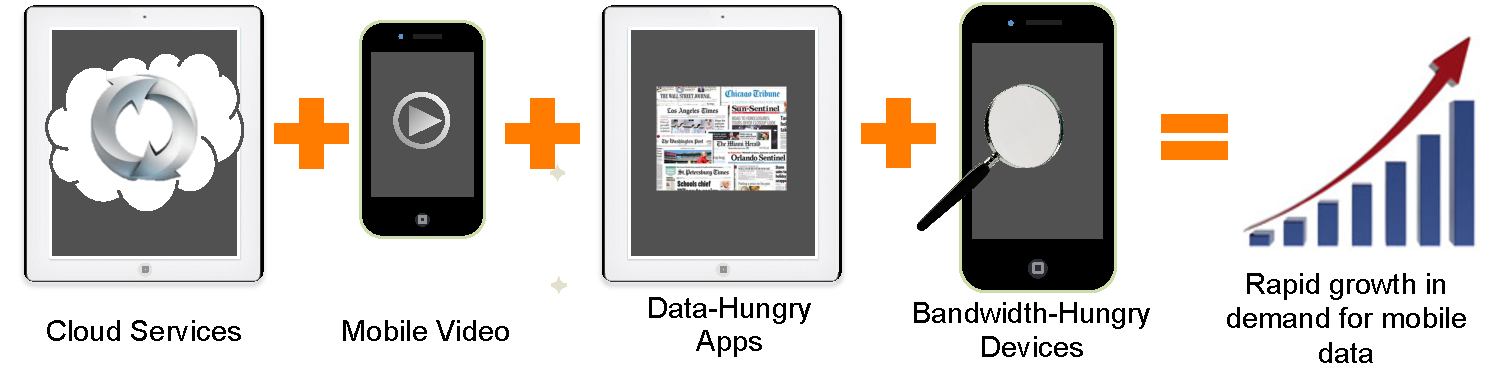
\includegraphics[width = 0.9\textwidth]{Figures/Driving_factors.pdf}
\vspace{-0.1in}
\caption{Factors driving the demand for mobile data.}
\label{fig:driving_factors}
\vspace{-0.05in}
\end{figure}

{\bf\emph{Cloud Services and M2M Applications:}}
Cloud-based services that synchronize data across multiple mobile devices, such as iCloud, Dropbox, and Amazon�s Cloud Drive, can be a significant factor in traffic growth for ISPs \cite{icloud}. Similarly, machine-to-machine (M2M) applications that generate data intermittently (e.g., sensors and actuators, smart meters) or continuously (e.g., video surveillance) often load the network with large signaling overhead \cite{BellLabs}.  However, these traffic types also have some intrinsic time elasticities that create opportunities for intelligently shifting them to low-congestion times through pricing incentives. 

{\bf\emph{Mobile Videos:}}
Video has also been a major contributor to mobile data traffic growth, accounting for 51 percent of global mobile data traffic at the end of 2012. It is expected to account for 66 percent of global mobile data traffic by 2017 \cite{CiscoVNImobile}. A study by Gartner \cite{Gartner2012} states that the worldwide mobile video market had 429 million mobile video users in 2011, projected to grow exponentially to 2.4 billion users by 2016. Smartphones and tablet sales will contribute 440 million new mobile video users during the forecast period. The report also forecasts that the worldwide share of mobile video connections on 3G/4G will increase from 18\% in 2011 to 43\% in 2015 \cite{Goog-mobile}. These growth rates are being further fueled by mobile video content delivery via mobile-optimized websites and video advertisements.

{\bf\emph{Capacity-Hungry Applications:}}
The popularity of handheld devices has led to rapid growth in the development of other bandwidth-hungry applications for social networking, music, personalized online magazines, etc. in addition to file downloads and video streaming. Virgin Media Business reports that the average smartphone software uses 10.7 MB per hour, with the highest-usage app, Tap Zoo, consuming up to 115 MB/hour. In the current ecosystem, app developers do not have enough incentives to account for network conditions, and consequently many smartphone apps are not optimized for bandwidth consumption.

{\bf\emph{Bandwidth-Hungry Devices:}}
The widespread adoption of handheld devices, equipped with powerful processors, high-resolution cameras, and larger displays, has made it convenient for users to stream high-quality videos and exchange large volumes of data.  Data from laptops with 3G dongles and netbooks with wireless high-speed data access contributes the most to wireless network congestion \cite{BellLabs}.  As for smartphones, Cisco projects that the average monthly data usage will rise from 150 MB in 2011 to 2.6 GB in 2016 \cite{CiscoVNImobile}.  New features like Siri on the iPhone 4S, which has doubled Apple users' data consumption, are driving this growth \cite{siri}.

The key takeaways from the above discussion of the various factors contributing to network congestion are:
\begin{itemize}
\item Different types of applications and services have different levels of time elasticity of demand (e.g., cloud backup versus financial applications).
\item There is a great variance in the rate of growth of different types of applications (e.g., demand for mobile videos is growing fast).
\item Different applications consume bandwidth at different rates and have a large variance in QoE requirements (e.g., many apps are not optimized for bandwidth while some well-designed apps can adapt to available network QoS). 
\item There is a growing variance in the bandwidth requirements of different smart devices (e.g., iPad versus iPhone versus feature phones).
\end{itemize}
These factors contribute to the need for smarter data plans that can account for the variances across users' QoE needs, time elasticity of demand, application traffic characteristics and their willingness to pay for the service.

%These developments have led ISPs to view pricing as their ultimate congestion management tool, paving the way for the adoption of Smart Data Pricing (SDP) measures, such as time-dependent and usage-based pricing.
Before delving deeper into SDP's promise in addressing congestion issues \cite{SDPForum}, in the next section we first explore how these trends are impacting the various stakeholders of the network ecosystem, i.e., network operators, consumers, app developers, and content providers.

\section{Impact on the Network Ecosystem}\label{sec:threats}



%To understand the implications of these factors, we need to first look at the impact that this growth is having on the various stakeholders of the Internet ecosystem before delving deeper into the promises that \emph{Smart Data Pricing} (SDP) holds \cite{SDPForum}. In the following discussion, we explore the current challenges and threats from the perspective of carriers, consumers, and content providers.

%The Internet ecosystem today suffers from threats to both its \emph{sustainability} and \emph{economic viability}. The sustainability concern is due to the near doubling of demand for mobile data every year  \cite{CiscoVNI}, which brings into question the feasibility of finding any purely technical solutions to this problem. Additionally, changes in the policy to make more spectrum available, although useful, is unlikely to provide any long-term solution.  For example, the US Government's initiative in releasing an additional 50 MHz of spectrum into the market for six carriers to compete for is widely viewed as being quite insufficient \cite{tollfree}. 

%The latter concern regarding the economic viability of Internet access is due to the large overage charges and throttling that ISPs (e.g., AT\&T and Verizon) are now imposing on their customers to penalize demand. To understand the implications of these factors, we need to first look at the impact that this growth is having on the various stakeholders of the Internet ecosystem before delving deeper into the promises that \emph{Smart Data Pricing} (SDP) holds \cite{SDPForum}. In the following discussion, we explore the current challenges and threats from the perspective of carriers, consumers, and content providers.

\subsection{ISPs' Traffic Growth}    

%The Cisco Visual Networking Index \cite{CiscoVNI} predicted in 2012 that mobile data traffic\footnote{``Mobile data traffic'' includes handset-based data traffic, such as text messaging, multimedia messaging, and handset video services, as well as traffic generated by notebook cards and mobile broadband gateways.} will grow at a compound annual growth rate (CAGR) of 78\% between 2011 and 2016, reaching a volume of 10.8 exabytes per month in 2016. By that time, Cisco predicted that the average smartphone user will consume 2.6 GB per month, as opposed to 150 MB/month in 2011 \cite{CiscoVNImobile}. This growth in per-device data consumption is fueled by the demand for bandwidth-intensive apps: for example, Allot Communications reports that usage of Skype's video calling service grew by 87\% in 2010, while usage of Facebook's mobile app grew by 267\% \cite{allot}. Devices themselves are also contributing to the increase in traffic volume; Apple's iPad 3 quadrupled the screen resolution from the iPad 2, allowing videos of higher quality to be streamed to the device \cite{apple}.

%Cisco predicted that by 2016, Wi-Fi and mobile data will comprise 61\% of all Internet traffic, with wired traffic comprising the remaining 39\% \cite{CiscoVNI}. Although the faster growth rate in mobile data traffic is a major concern, growing congestion on wired networks both at the edge and in the networks' middle mile also poses a significant problem. 
%-- consumer traffic from fixed IPs is expected to grow at a CAGR of 28\% per year from 2011-2016, while managed IP traffic is expected to sustain a 21\% CAGR \cite{CiscoVNI}.\footnote{Cisco's definition of ``consumer'' includes fixed IP traffic generated by households, university populations, and Internet cafes, `while ``managed IP'' includes corporate IP WAN traffic and IP transport of TV and VoD.}) 

By 2016, ISPs are expected to carry 18.1 petabytes per month in managed IP traffic.\footnote{Cisco's definition of ``managed IP'' includes traffic from both corporate IP wide area networks and IP transport of television and video-on-demand.} But this growth is causing concern among ISPs, as seen during Comcast's initiative to cap their wired network users to 300 GB per month \cite{Comcast-cap}. Even back in 2008, Comcast made headlines with their decision (since reversed) to throttle Netflix as a way to curb network congestion \cite{Comcast-Level3}. Video streaming from services like Netflix, Youtube, and Hulu, are a major contributor to wired network traffic. In fact Cisco predicts that by 2016 fixed IPs will generate 40.5 petabytes of Internet video per month \cite{CiscoVNI}.
  
Rural local exchange carriers (RLECs) are also facing congestion in their wired networks due to the persistence of the middle-mile problem for RLECs. Although the cost of middle mile bandwidth has declined over the years (because of an increase in the DSL demand needed to fill the middle mile), the bandwidth requirements of home users have increased quite sharply \cite{vglass-2}. Still, the average speed provided to rural customers today fails to meet the Federal Communications Commission's (FCC) broadband target rate of 4 Mbps downstream speed for home users. The cost of middle mile upgrades to meet this target speed will be substantial and is a barrier to digital expansion in the rural areas \cite{vglass-2}. Research on access pricing as a mechanism to bring down middle mile investment costs by reducing the RLEC's peak capacity and over-provisioning needs can therefore also help in bridging the digital divide.

\subsection{Consumers' Cost Increase}

Network operators have begun to pass some of their network costs to consumers through various penalty mechanisms (e.g., overage fees) and increasing the cost of Internet subscriptions. For instance, when Verizon announced in July 2012 that they were offering shared data plans for all new consumers and discontinuing their old plans, many consumers ended up with higher monthly bills \cite{nyt-shared}. To remain within monthly data caps, consumers are increasingly relying on usage-tracking and data compression apps (e.g., Onavo, WatchDogPro, DataWiz) \cite{datawiz} that help to avoid overage fees. Such trends are common in many parts of the world; in South Africa, for instance, consumers use ISP-provided usage-tracking tools \cite{chetty2012you} to stay within the data caps. Similarly in the U.S., research on in-home Internet usage has shown that many users are concerned about their wired Internet bills and would welcome applications for tracking their data usage and controlling bandwidth rates on in-home wired networks \cite{chetty2011my,netlimiter}. Empowering users to monitor their data usage and control their spending has led to a new area of research that considers economic incentives and human-computer interaction (HCI) aspects in a holistic manner \cite{sigchi}. 

\subsection{Application Developers' Perspective}

Introducing pricing schemes that create a feedback-control loop between the client side device and network backend devices requires new mobile applications that will support such functionalities. However, most mobile platforms in use today (e.g., iOS, Android, and Windows) have different levels of platform openness.  The iOS platform for iPhones and iPads has several restrictions: it strictly specifies what kind of applications can run in the background and further prevents any access other than the standard application programming interfaces (APIs). For example, obtaining an individual application's usage and running a pricing app in the background are prohibited. By contrast, the Android and Windows platforms allow these features, e.g., introducing an API to report individual applications' usage to third-party apps.

An interesting direction to overcome these limitations is to initiate the creation of open APIs between user devices and an ISP's billing systems. For example, this can allow the user devices connected to the ISP's network to easily fetch current pricing, billing, and usage information from the network operator, while also allowing the ISP to easily test and deploy new pricing schemes through the standardized interface. Such an API would foster innovations in pricing for both consumers and providers.

Additionally, new pricing plans create an opportunity for developers to optimize their app according to changing pricing conditions. For instance, some apps that require preloading content, such as magazine apps, might time these preloading downloads so as to coincide with lower-price times, thus saving users money \cite{sigchi}. This sensitivity to price might even improve users' experience, as lower prices generally occur during times of lower congestion and higher throughput. Shifting usage so as to save money could be especially significant for video apps, as these tend to have higher usage volumes.\footnote{Some video apps cannot shift usage due to legal restrictions on caching content. However, many apps like YouTube own the rights to their video content.} Such adaptation would also require an API allowing apps to access the network prices in real time.

% Wireless ISPs' current billing systems (including 2G, 3G, and 4G) heavily depend on the RADIUS (Remote Authentication Dial In User Service) protocol, which supports centralized Authentication, Authorization, and Accounting (AAA) for users or devices to use a network service \cite{rfc2865}. In particular, RADIUS accounting \cite{rfc2886} is well suited to support usage-based pricing, since it can keep track of the usage of individual sessions belonging to each user. Interim-update messages to each session can be sent periodically to update the usage information. However, RADIUS accounting lacks support for dynamic pricing plans, which require time-of-day usage at various time scales\footnote{Note that interim update messages are sent periodically when a session joins the system, and hence, the time interval for interim updates should be kept low to support sending time-of-day usage, which may introduce significant control overhead.} Therefore, extending these protocols to support new pricing mechanisms, standardizing interfaces, and the creation of open APIs between network operators and application developers will be interesting directions for future research in this area.
  
%Additionally, empowering users to monitor and control of their data usage requires understanding of the intersection between the economic incentives and human-computer interaction (HCI) aspects \cite{sigchi}. 

\subsection{Software/Hardware Limitations}

Wireless ISPs' current billing systems (including 2G, 3G, and 4G) heavily depend on the RADIUS (Remote Authentication Dial In User Service) protocol, which supports centralized Authentication, Authorization, and Accounting (AAA) for users or devices to use a network service \cite{rfc2865}. In particular, RADIUS accounting \cite{rfc2886} is well suited to support usage-based pricing, since it can keep track of the usage of individual sessions belonging to each user. Yet individual session lengths are often quite long, making it difficult to retrieve usage at the smaller timescales needed for dynamic pricing.

RADIUS account sessions are initiated by the Network Access Server (NAS) when a user first attempts to connect to the network: the NAS sends a user's login credentials to the RADIUS server, which compares the credentials to a secure database. The RADIUS server then \emph{authenticates} the session and \emph{authorizes} it to access different functionalities on the network. Once this session has been initiated, a start record is created in the RADIUS logs. Interim \emph{accounting} request messages can be sent periodically to update the usage information. When the end user terminates the connection, the NAS sends a stop message to the RADIUS server and a stop record is created that stores the total usage volume of that session. Since these RADIUS sessions can have very long durations, up to several hours, RADIUS logs cannot be used to calculate usage at smaller timescales.\footnote{Note that interim update messages are sent periodically when a session joins the system, and hence, the time interval for interim updates should be kept low to support sending time-of-day usage, which may introduce significant control overhead.} Moreover, the RADIUS log has no information on the type of application(s) corresponding to each session. While one session may encompass usage from multiple apps used in parallel, in some cases individual apps initiate new sessions; thus, the concept of a ``session'' cannot be definitively tied to an individual app \cite{rfc2886}.

Changing the RADIUS protocol to deliver usage estimates at a smaller time granularity would require significant overhead in both control signaling and storing RADIUS records. A perhaps easier alternative would be to record usage at the network edge, i.e., on client devices--such functionality already exists, but this approach would be vulnerable to users' deliberately falsifying the usage recorded on their device. Similarly, RADIUS logs do not contain any information on per-application usage, but client devices can easily obtain this information. Thus, application-specific pricing could also benefit from usage tracking functionalities on the end user devices. Some verification procedures could be implemented to guard against user tampering, e.g., comparing the total monthly usage measured by RADIUS servers and client devices, but would require careful design and might not be completely secure.

% Another interesting direction is the creation of an open API between user devices and an ISP's billing systems. The open API will foster innovations in pricing for both consumers and providers. For example, the user devices connected to the ISP's network can easily fetch their pricing, billing, and usage information from the network, and the ISP can also easily test and deploy new pricing schemes through the standard interface.

%\emph{Reducing App Bandwidth:} In light of the growing demand for mobile data, a natural question is whether more efficient app development can reduce apps' traffic volume, and more fundamentally whether bandwidth consumption is a consideration during app development. A small online survey of mobile app developers revealed divided opinions \cite{sigchi}. For example, one iOS developer with 4 years of experience and 12 apps told us �No, most app developers do what must be done. Only experienced app developers will look for ways to reduce bandwidth usage� (D1). Developer D2 with 5 years of experience echoed this view: �User experience and interface seem to be the main need in the App Store.� But another iOS developer with 2 years of experience and 3 apps opined that apps do consider data usage: �Bandwidth overhead is very important to the user and should thus be important to the developer too� (D3). However, he added that the �previous version of Facebook app was - because of all UIWebViews - very slow on mobile connections. Reducing the bandwith by using native UI interfaces gave a huge speed bump.� When asked whether TDP plans will hurt app development, developer D1 felt that developers will adapt to new plans, while D3 felt that it won�t have any effect: �I don't think that developers will change their design just because of changes in data plans.�
%
%The developers also provided examples of apps that can actually benefit from TDP: �applications that can cache websites and newsfeeds to read later� (D3), �Dropbox or any file sharing and backup app� (D2), and apps like YouTube that can choose �different resolutions depending on network availability� (D1). But, developer D3 opined: �The Internet�s greatest advantages above all other media is, that it's always up-to-date. It is the fastest media and adding such plans will cut off this advantage. The users want to be up-to-date.� 


\subsection{Content Delivery Issues}

Any change in access pricing has to be studied in the larger context of Internet's net-neutrality and openness. These discussions center around the issues of (a) who should pay the price of congestion (i.e., content providers or consumers) and (b) how such pricing schemes should be implemented (i.e., time-of-day, app-based bundles, etc.).  The major concern with policy change is the possibility of paid prioritization of certain content providers' traffic, price discrimination across consumers, and promoting anti-competitive behavior in bundled offerings of access plus content.  While such developments can indeed hurt the network ecosystem, one aspect that should receive more attention is the threat to data usage even under simple usage-based or tiered data plans.  As Internet users become more cautious about their data consumption \cite{BostonGlobe}, content providers are providing new options to downgrade the quality of experience (QoE) for their users to help them save money.  For instance, Netflix has started allowing ``\emph{users to dial down the quality of streaming videos to avoid hitting bandwidth caps}''  \cite{Newman}. Additionally, it is ``\emph{giving its iPhone customers the option of turning off cellular access to Netflix completely and instead relying on old-fashioned Wi-Fi to deliver their movies and TV shows}'' \cite{Fitchard}.  Thus, the ecosystem today is being driven by an attitude of penalizing demand and lessening consumption through content quality degradation. 

Network researchers are investigating these issues broadly along two lines of work: (i) opportunistic content caching, forwarding, and scheduling, and (ii) budget-aware online video adaptation. Opportunistic content delivery involves the smart utilization of unused resources to deliver higher QoE; for example, to alleviate the high cost of bulk data transfers, Marcon et al. \cite{marcon2012netex} proposed utilizing excess bandwidth (e.g., at times of low network traffic) to transmit low-priority data. Since this data transmission does not require additional investment from ISPs, they can offer this service at a discount, relieving data transfer costs for clients. While utilizing excess bandwidth introduces some technical issues (e.g., the potential for resource fluctuations), a prototype implementation has shown that they are not insurmountable \cite{laoutaris2011inter}. The second stream of works on online video adaptation systems, such as Quota Aware Video Adaptation (QAVA) \cite{Jiasi}, have focused on sustaining a user's QoE over time by predicting her usage behavior and leveraging the compressibility of videos to keep the user within the available data quota or her monthly budget.  The basic idea here is that the video quality can be degraded by non-noticeable amounts from the beginning of a billing cycle based on the user's predicted usage so as to avoid a sudden drop in QoE due to throttling or overage penalties when the monthly quota is exceeded. This relates to the SDP theme of enabling self-censorship of usage and QoE on the client side device through user-specified choices. %A common feature of these new research directions is that they address the concerns of consumers and content providers by accounting for both technological and economic factors.

\subsection{Regulatory Concerns}

Pricing in data networks has remained a politically charged issue, particularly for pricing mechanisms that could potentially create incentives for price discrimination, non-neutrality, and other anti-competitive behavior through app-based pricing or bundling of access and content.  Academics have already cautioned that the ongoing debate on network neutrality in the U.S. often overlooks service providers' need for flexibility in exploring different pricing regimes \cite{Yoo}:   
\begin{quote}
\emph{Restricting network providers' ability to experiment with different protocols may also reduce innovation by foreclosing applications and content that depend on a different network architecture and by dampening the price signals needed to stimulate investment in new applications and content.}
\end{quote}

But faced with the growing problem of network congestion, there has been a monumental shift in the regulatory perspective in the US and other parts of the world.  This sentiment was highlighted in FCC Chairman J. Genachowski's 1 December 2010 statement \cite{FCC}, which recognizes \emph{``the importance of business innovation to promote network investment and efficient use of networks, including measures to match price to cost."}  



\section{Smart Data Pricing}\label{SDP}

%The demand for data is growing rapidly in both wired and wireless networks. This growth is primarily driven my the rise of mobile video, bandwidth-hungry apps, bulk transfer to the cloud, and user-friendly interfaces of smart devices. The Cisco Visual Networking Index predicts that data from mobile devices will grow to a volume of 10.8 exabytes per month in 2016, while wired network traffic will increase at a compound annual growth rate of 28\% per year \cite{CiscoVNI}. 

%The predicted doubling of demand for mobile data every year also means that technical solutions and spectrum reallocation are going to be insufficient to meet the growing needs of the users. ISPs' (Internet service providers) are therefore turning to new pricing plans in an effort to manage their demand for data and match their prices to cost \cite{comm-mag}. Such policies include charging based on usage volume, throttling users' bandwidth, and imposing caps on monthly usage.  Figure \ref{fig:timeline} provides an overview of the rapidly evolving pricing and demand control practices of the major U.S. ISPs since 2008. In fact, over the past few years, ISPs around the world have started to offer innovative pricing plans, including usage-based and app-based pricing to tackle the problem of network congestion \cite{computing-survey}. 

 \begin{figure}
\centering
\includegraphics[width = 0.85\textwidth]{Figures/Timeline.pdf}
\vspace{-0.1in}
\caption{Broadband pricing plans offered by major U.S. ISPs, 2008 - 2013.}
\label{fig:timeline}
\vspace{-0.05in}
\end{figure}

Broadband access pricing and demand control practices have rapidly evolved among U.S. ISPs since 2008, as seen in Figure \ref{fig:timeline}. Over the past few years, ISPs around the world have started to offer innovative pricing plans, including usage-based and app-based pricing to tackle the problem of network congestion \cite{computing-survey}. Smart Data Pricing (SDP) \cite{SDP2013} is an umbrella term for a suite of pricing and policy practices that have    
been proposed in the past or are being explored as access pricing options by operators instead of the traditional flat-rate model. Such SDP models can include any or of the following mechanisms or a combination, which will be discussed later in the chapter: (a) Usage-based pricing/metering/throttling/capping, (b) Time/location/congestion-dependent pricing, (c) App based pricing/sponsored access, (d) Paris metro pricing, (e) Quota-aware content distribution, (f) Reverse billing or Sponsored Content. SDP does not even need to be an explicit pricing mechanism; it can be another form of innovative congestion management like WiFi offloading or ``fair-throttling''\footnote{Fair throttling involves accounting for user's usage history of contributing to congestion in determining what share of available bandwidth the user should receive in a congested time.}.

The basic ideas of congestion pricing have received much attention as a research topic both in computer networks and information systems literature, and are once again getting a fresh look from academics in recent years. Given the change in the economic and regulatory environment of Internet pricing, it is likely that some of the ideas will be realized in future data plans. However, research in the design of such smart data pricing plans should account for some new factors: (i) the growth in traffic with high time-elasticity of demand (e.g., downloads, P2P, cloud backup, M2M) and the ability to schedule such traffic to a less congested time without user-intervention, (ii) revisiting the issue of dividing the elements of a congestion control-feedback loop between the network backend and the smart end-user devices, (iii) development of new system architectures to deploy these pricing ideas and demonstration of their potential benefits through field trials. In other words, it requires understanding both the \emph{economic theory} of pricing models as well as the \emph{systems engineering} and \emph{human-computer interaction} aspects of realizing such data plans. These require a multi-disciplinary approach in SDP research that bridges theory, systems, and user trials by drawing on economic theory, network engineering and user behavioral studies in a collaborative environment, as shown in Figure \ref{fig:theme}.

 \begin{figure}
\centering
\includegraphics[width = 0.5\textwidth]{Figures/Sdp-theme.pdf}
\vspace{-0.1in}
\caption{Smart Data Pricing research components}
\label{fig:theme}
\vspace{-0.05in}
\end{figure}

% Unfortunately, most academic materials presently available online tend to only provide just enough background on congestion pricing models from a theoretical perspective, rather than taking a more holistic approach.  In particular, most of the materials on economic aspects of the Internet available to students and faculties are either technical papers from conferences such as ACM SIGCOMM, NetEcon, CoNEXT, INFOCOM or edited books of workshop proceedings \cite{MIT}. It is arguably fair to say that most networking textbooks do not cover this important topic in enough depth, and this lack of background materials at the graduate level is indeed a serious issue that the community is now reckoning with. There is a growing realization in the network research community about the need to include network economics as an integral part of engineering curriculum given the complex interplay between technological and economic factors. To this end, we propose to bridge this gap by contributing a chapter that exclusively focuses on the network economics of smart pricing practices for the Internet. 


%The key elements of this chapter will be: (i) a detailed overview of pricing proposals, (ii) system design considerations in smart pricing, and (iii) human factors and results of pricing trials of SDP plans. % The authors have been deeply involved in studying pricing plans, published survey articles and research papers on SDP, and have conducted real trials of SDP with ISPs in US and India, which will inform the contents presented in this contribution.   Additionally, the authors will seek inputs from their collaborators and peers  with whom they have been working closely for network economics research,  especially Prof. Andrew Odlyzko of the University of Minnesota and Prof. Roch Guerin of the University of Pennsylvania, both of whom were invited keynote speakers at the first SDP workshop hosted by the authors in Princeton University in 2012 \cite{SDPForum}. We would also provide a summary of open questions and challenging directions in network pricing, along with supplementary background materials, that can benefit graduate students in identifying new research directions to pursue.

% In the following sections, we first provide an overview of the driving factors behind network congestion in Section \ref{sec:factors}. This rising demand for bandwidth has led to new threats to the current Internet ecosystem: ISPs are increasingly feeling a capacity crunch on their networks, leading to new pricing plans that have raised concerns among consumers hit with these new forms of pricing. Content providers, whose videos and other content make up the increased traffic volume that consumers are demanding, also have a stake in this evolving ecosystem, as do application developers and government regulators attempting to find a balance between ISP capacity concerns and Internet availability. We discuss these different perspectives in Section \ref{sec:threats}. In Section \ref{sec:econ}, we consider a few examples of SDP to illustrate key economic concepts essential for understanding the SDP literature. Section \ref{sec:congestion} gives an overview of this literature, including some pricing plans from the electricity and transportation industries that can be applied to broadband pricing. We then delve into one such pricing plan, day-ahead time-dependent pricing, in order to illustrate the end-to-end nature of an SDP deployment, which requires developing pricing algorithms, designing an effective interface for communicating those prices to users, and implementing an effective system to communicate between an ISP and its users. Finally, we point to some (of many) research questions for broadband access pricing that have yet to be answered.



\section{A Review of Smart Data Pricing}\label{sec:congestion}

Smart data pricing encompasses a wide variety of different pricing algorithms and proposals. In this section, we briefly discuss some of these ideas, following the taxonomy given in Figure \ref{fig:taxonomy}. We include a brief overview of related pricing plans in the electricity and transportation industries, which can help yield insights into the feasibility of various forms of SDP for data, as well as ideas for new pricing plans. Other, more thorough reviews may be found in \cite{CourcoubetisWeber,sen2013survey,Songhurst}.

\begin{figure}
\centering
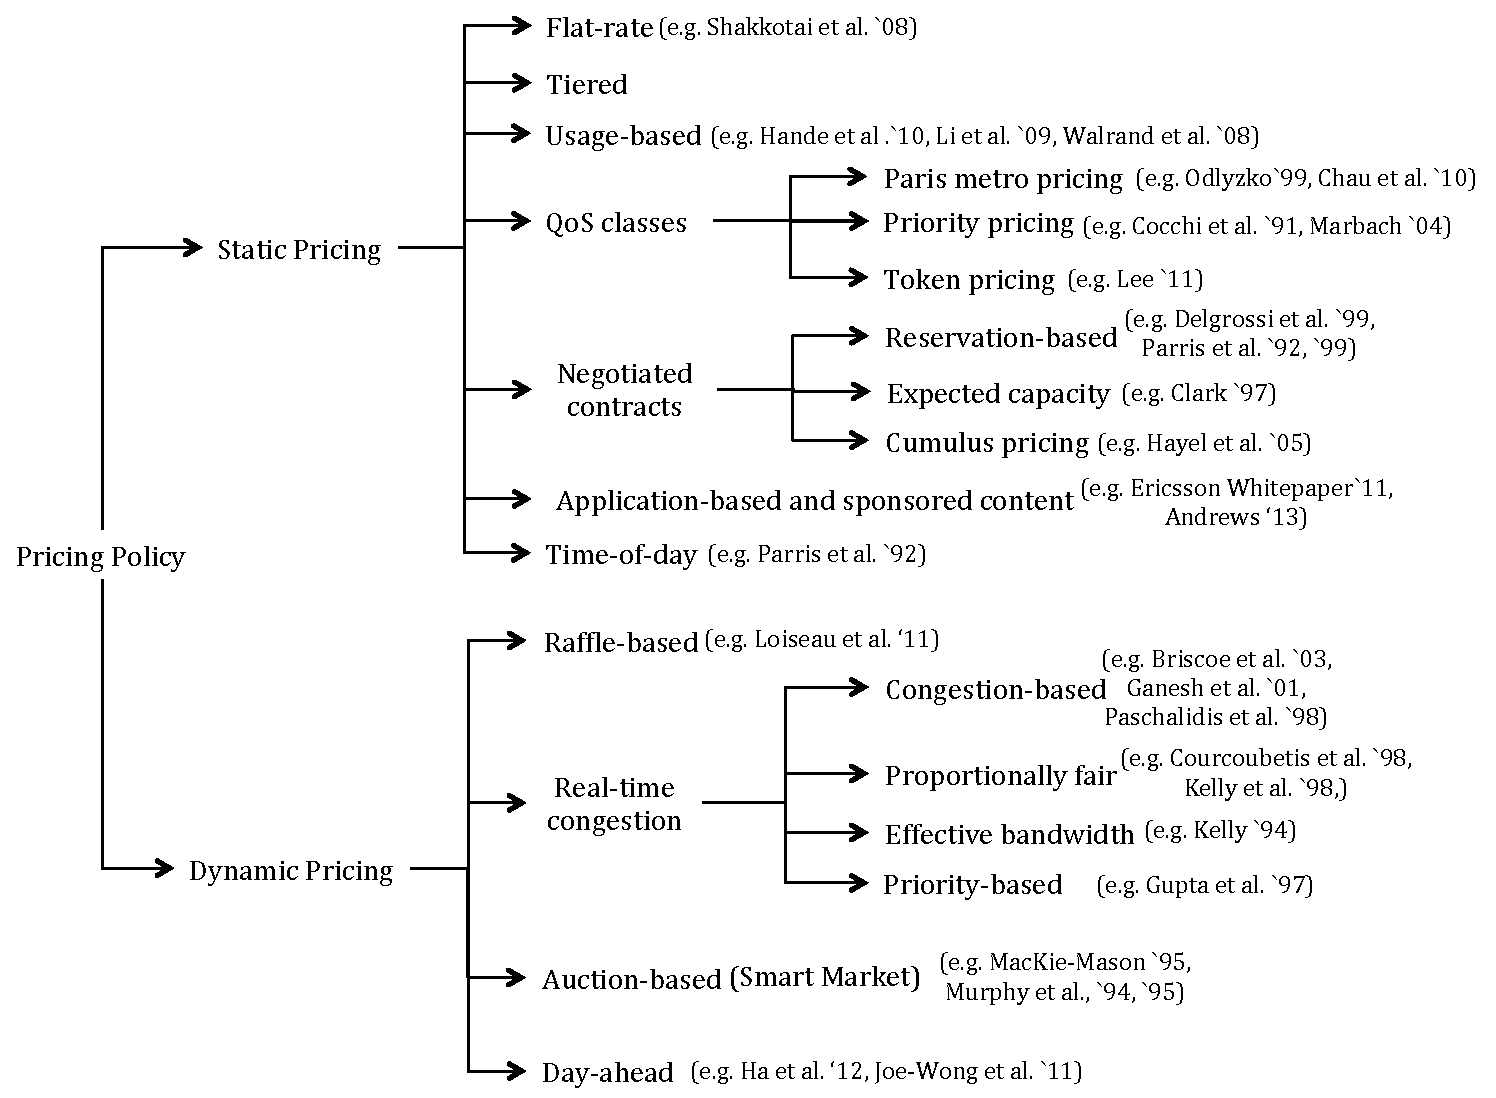
\includegraphics[width = 0.8\textwidth]{Figures/Taxonomy.pdf}
\caption{Examples of broadband pricing plans proposed in the research literature.}
\label{fig:taxonomy}
\end{figure}

A primary goal of SDP is to create the right incentives (or price points) for users to modify their usage behavior so as to help ISPs with better resource allocation and utilization. But creating these incentives requires ISPs to account for users' responses to the prices offered. Of particular relevance is the timescale associated with the pricing mechanism -- do the prices continually change as the network load changes? If so, how frequently and by how much? How to balance the trade-offs between users' reluctance to real time dynamic pricing and the inability of static pricing to exploit the time elasticity of demand of different applications in congested times? How to balance the trade-offs between the users' need for transparency and control over her usage and the need for automation in dynamic pricing scenarios? 

\emph{Static pricing} plans are those that change prices on a relatively longer timescale, e.g., months or years: the offered prices do not vary with immediate changes in the network congestion level. The popularity of these plans arises from the certainty they provide to a user's expected monthly bill. For instance, tiered data plans with pre-specified rates are prevalent in the United States, and several European and Asian ISPs offer usage-based pricing in which users are charged in proportion to their usage volume. But such usage-based pricing leaves a timescale mismatch: ISP revenue is based on monthly usage, but peak-hour congestion dominates its cost structure (e.g., network provisioning costs increase with the peak-hour traffic). Another well-known pricing plan is time-of-day (ToD) pricing, in which users are charged higher prices during certain ``peak'' hours of the day. But even with ToD pricing, the hours deemed as ``peak'' are fixed, which results in two challenges. First, traffic peaks arise in different parts of the network at different times, which can be hard to predict in advance and could end up creating two peaks during the day--one during peak periods, for traffic that cannot wait for several hours for lower-price periods, and another peak during discounted ``off-peak'' periods for time-insensitive traffic. Such patterns have been observed in dynamic pricing for voice calls in operational networks \cite{Economist}. We discuss several of these existing static pricing plans and proposals in greater detail in Section \ref{sec:static}.

\emph{Dynamic pricing} takes the ToD idea further in that it does not pre-classify peak and off-peak periods, instead adjusting prices at a finer timescale or by location in response to the network congestion. However, prices that vary depending on the current network load can be sometimes inconvenient for users.  Hence, dynamic pricing variants for SDP, such as automated ``smart market" \cite{MacKie-Mason,Murphy-Murphy}, raffle-based pricing \cite{loiseau2011incentive}, and day-ahead pricing \cite{ha2012tube}, have been proposed to guarantee the prices a day in advance to give users some certainty about the future prices on offer. Each day, new prices are computed for different times (e.g., hours) of the next day, based on predicted congestion levels.  A detailed discussion on these dynamic pricing proposals will be provided in Section \ref{sec:dynamic}.


\subsection{Static Pricing}\label{sec:static}

Due to the fixed nature of their prices, static data plans do not generally allow ISPs to adapt to real-time congestion conditions. In particular, the ISP cannot prevent or alleviate network congestion at peak times by manipulating the prices. On the other hand, static pricing tends to be more acceptable to users, as it offers more certainty and is simpler than dynamically changing prices. Indeed, the most basic form of static pricing, \emph{flat pricing}, is also the most simple for users, though it does not impose any sort of usage incentives \cite{shakkotai}. Some other important examples of static pricing include the following:

\textbf{\emph{Usage-based:}}
In its purest form, usage-based pricing charges users in proportion to the amount of data that they consume, without regard to the type of data (e.g., application) or time of consumption. The principal advantage of such a pricing plan lies in its relative simplicity: it imposes a monetary penalty on heavy (i.e., high-usage) users to reduce congestion \cite{hande,Li}, but also penalizes users even when the network is lightly loaded. Moreover, usage-based pricing requires users to keep close track of their usage in order to determine how much they have spent on data \cite{walrand}.

\textbf{\emph{Tiered:}}
A more common variant of pure usage-based pricing is tiered pricing, in which users pay a fixed amount of money for a monthly \emph{data cap} (e.g., \$30 for 3GB). This fixed fee covers usage up to the cap, after which users may pay another fixed fee to increase the cap by a discrete amount, e.g., \$10 per extra GB. Thus, tiered or capped pricing can be viewed as a discretization of usage-based pricing. Many ISPs have adopted such a pricing plan or another variant in which the data cap is shared across several devices (i.e., a \emph{shared data plan}). Like usage-based pricing, tiered pricing is simple for users to understand and penalizes heavy usage. %; however, it also puts less burden on users to keep track of their usage in order to calculate their monthly bills. % Yet neither usage-based nor tiered pricing prevents users from using the network at the same time, and thus do not significantly help reduce the peak congestion. 

\textbf{\emph{Quality of Service (QoS) classes:}}
Some static pricing plans offer multiple traffic classes with different qualities of service (QoS). A simple differentiated pricing plan is \emph{Paris metro pricing} (PMP), which is named after an actual pricing practice on the Paris metro in the 1900s \cite{Odlyzko}. In Paris metro pricing, the ISP separates data traffic into different logical traffic classes and charges different prices for logically separate traffic classes (i.e., each class is identical to the others in their treatment of data packets). Only users willing to pay a higher price will adopt this traffic class, which leads to a better QoS due to fewer users. But one of the key issue of academic debate related to PMP has been its viability, namely,  whether it is a mechanism to increase the profits for service providers, or whether it achieves higher social welfare. As pointed out in \cite{Chiu2010}, the conclusions of this debate depend on how users react to the congestion externality of the underlying system. Other researchers have investigated more direct forms of QoS pricing, in which users can indicate their desired QoS in their packets and are charged a higher per-byte fee for higher QoS \cite{Cocchi1,Marbach,M3I}. %Determining users' optimal QoS decisions and the per-byte fees to charge are non-trivial research questions.

%each of which is identical in its treatment of data packets but charges users differently.  Thus, users willing to pay more will select the more expensive, and hence less congested, logical traffic class.

Another form of QoS pricing is \emph{token pricing}, in which users receive tokens at a fixed rate (e.g., 1 per minute) \cite{Token}. Users can then spend these tokens to send some of their traffic at a premium QoS; users can choose the timing of these premium sessions, e.g., to coincide with their individual priorities and preferences. %One can then examine users' spending decisions and their implications for congestion reduction.

\textbf{\emph{Negotiated contracts:}}
In these types of pricing schemes, users pre-negotiate contracts with the ISP regarding the price of sending traffic over the network. The main research question for such contracts is then characterizing this user-ISP interaction and both parties' optimal decisions. For instance, in \emph{reservation-based pricing}, users specify a monthly budget for data; the ISP can then accept or reject users' connections based on users' remaining budget and the real-time network congestion \cite{Delgrossi,PKF, ParrisF}. 

In \emph{expected capacity pricing}, Clark proposed a mechanism in which users similarly negotiate a price in advance based on an ``expected'' quality of service (e.g., file transfer time), so that at congested times the ISP can freely allocate network resources based on whether a given packet lies ``within'' a user's purchased traffic profile \cite{DDClark}. The goal of this pricing scheme is to ``\emph{provide additional explicit mechanisms to allow users to specify different service needs, with the presumption that they will be differentially priced} \cite{DDClark}." Expected capacity pricing allows users to explicitly specify their service expectation (e.g., file transfer time), while accounting for differences in applications' data volume and delay tolerance. The idea is that by entering into profile contracts for expected capacity with the operator, different users should receive different shares of network resources when the network gets congested \cite{Songhurst}.  
One specific proposal to realize this service involved traffic flagging (i.e., each packet is marked as being \emph{in} or \emph{out} of the user's purchased profile, irrespective of network congestion level) by a traffic meter at access points where the user's traffic enters the network. This is followed by congestion management at the switches and routers where packets marked as \emph{out} are preferentially dropped during congested periods, but are treated in an equal best-effort manner at all other times.  The expected capacity is thus not a capacity guarantee from the network to the user, but rather a notion of the capacity that a user expects to be available and a set of mechanisms that allow the user to obtain a different share of the resource at congested times.  
%This pricing can be simply enforced at the router and switches of the network, and allows service providers to have more stable estimates of the future necessary capacity based on the total expected capacity sold, rather than the sum of peak rates of all users' access links.  A dynamic pricing version of the scheme has also been explored \cite{DDClark}. However, in order to implement this pricing scheme, the assignment of price values to expected capacity profiles requires further study.

An ISP offers similar contracts under \emph{cumulus pricing}, but users can re-negotiate the price after passing ``cumulus'' usage points \cite{Hayel}. Cumulus pricing consist of three stages: specification, monitoring, and negotiation. A service provider initially offers a flat-rate contract to the user for a specified period based on the user's estimate of resource requirements. During this time the provider monitors the user's actual usage and provides periodic feedback to the user (by reporting on ``cumulus points'' accumulated from their usage) to indicate whether the user has exceeded the specified resource requirements. Once the cumulative score of a user exceeds a predefined threshold, the contract is renegotiated. 

\textbf{\emph{App-based and sponsored content:}}
Different applications consume different amounts of data traffic (e.g., streaming video consumes much more data than retrieving emails). Some researchers have thus proposed app-based pricing, in which users are charged different rates for different apps \cite{Ericsson}. Such pricing plans also include ``zero-rated'' apps, whose traffic is free for the user. A variant of such pricing schemes is ``sponsored content'', in which a third-party (advertiser, content provider, or the ISP itself) ``sponsors'' some part of the traffic in return for accessing specific content or using data at less congested times. 

App-based plans have been offered in Europe, largely on a promotional basis. However, app-based pricing presents technical challenges for ISPs-- ISPs need to identify and track how much data each user consumes on specific applications, which may raise privacy concerns. Moreover, some apps open links in separate apps (e.g., links in Flipboard may open a separate Internet browser), creating confusion among users as to the app to which some traffic belongs, and whether this traffic counts towards the sponsored volume or not. Even in academia, sponsored content research is relatively sparse, though a few initial models have been developed \cite{andrewsSDP,hande2009network}.

\textbf{\emph{Time-of-day (ToD):}} ToD pricing charges users different usage-based rates at different times of the day (e.g., peak and off-peak hours) \cite{ParrisF}. The free nighttime minutes offered for voice calls by most US ISPs before 2013 are one simple form of ToD pricing. However, as the peak times and rates are fixed in advance, ToD pricing can end up creating two peaks, one during the ``peak'' period and one in the ``off-peak'' period; indeed, this phenomenon was observed in Africa when MTN Uganda offered discounted prices for voice calls made at night. 

Some ISPs offer two-period ToD pricing plans with different charging rates at day and night times.  For example, BSNL in India offers unlimited night time (2-8 am) downloads on monthly data plans of Rs 500 (\$10) and above. Other variations of ToD pricing are offered elsewhere; for instance, the European operator Orange has a ``Dolphin Plan''  for $\pounds$15 (\$23.50 USD) per month that allows unlimited web access during a ``happy hour'' corresponding to users' morning commute (8-9 am), lunch break (12-1 pm), late afternoon break (4-5 pm), or late night (10-11 pm). The underlying idea is to allow consumers to \emph{self-select} themselves into ``time-buckets" with QoE guarantees, with the hope of exploiting the variance in consumers' time-of-day preference to spread out demand more evenly over the day.


%Though the prices do change with time in ToD pricing, we list ToD pricing under static pricing due to the fact that the prices remain the same from day to day.

\subsection{Dynamic Pricing}\label{sec:dynamic}
Dynamic pricing allows prices to be changed in (near) real-time, which unlike static pricing allows an ISP to adjust its prices in response to observed network congestion. However, in doing so the ISP significantly complicates its pricing, making it much harder for users to understand. Thus, implementing and offering dynamic pricing plans requires ISPs to account for human factors that can make real-time changes in price more amenable to users. Some of the proposed dynamic pricing plans are discussed below:

\textbf{\emph{Real-time congestion:}} If ISPs can monitor their network for real-time signs of congestion, they can increase prices when congestion is observed, and decrease them when the traffic load is relatively light. Thus, there is a \emph{feedback loop} between ISPs offering prices and users correspondingly adjusting their usage \cite{Ganesh,Paschalidis}. This \emph{responsive pricing} sets prices so as to keep user demand under a certain level; if an ISP further chooses the prices so as to optimize a proportional fairness criterion on the amount of bandwidth allocated to different users, we obtain \emph{proportional fairness pricing} \cite{Courcoubetis,kelly1998rate,gibbens-kelly}. Many variants of responsive pricing have been proposed in the literature, principally as a congestion control mechanism; in practice, it would be impractical for users to manually respond to the prices offered for each Internet connection. Hence, automation of client devices (or agents) to intelligently adapt their data consumption will be necessary to realize such real-time pricing. But recent HCI studies \cite{chetty2010s,sigchi} have revealed complex patterns of household politics and user opinion regarding such decision-making about bandwidth consumption. In particular, there is a reluctance among users to delegate such bidding or scheduling to automated agents that stems from a conflict between the psychological assurance of manual control and the convenience of automation, which in turn depends on the perceived trust-worthiness of the underlying system. Many of the findings reported later in this chapter on user behavior and user interface design may serve as guidelines in designing user-friendly client-side agents to enable such pricing plans. 

Another form of congestion pricing, \emph{effective bandwidth pricing}, incorporates a form of QoS by charging users based on their connection's peak and mean rates \cite{Kelly-eff}. One can also explicitly incorporate different QoS by using \emph{priority pricing}, in which users can pay less by accepting a longer delay at congested times \cite{Gupta}. If the prices are chosen correctly, the system reaches an equilibrium, in which each user's packets are processed within the delay paid for.

\textbf{\emph{Auction-based:}} One disadvantage of real-time congestion pricing is that in practice, the ISP must set the prices (just) before observing user behavior. Since user demand can change with time, the ISP may end up setting non-optimal prices due to outdated assumptions of user demand. ``Smart market'' pricing addresses this slight delay with an auction-like scheme, in which users attach a bid to their packets that signifies their willingness to pay \cite{MacKie-Mason,Murphy-Murphy}. ISPs then admit a limited number of packets in descending order of the bids so as to limit network congestion. Users are charged the lowest bid admitted, which represents the ``cost of congestion.'' While smart market pricing allows true real-time pricing, it also requires automated agents on user devices to make bids as necessary and keep track of the final amount charged.

\textbf{\emph{Raffle-based:}} This is a variation of dynamic time-dependent pricing inspired by lottery reward mechanism. Under \emph{raffle-based pricing}, the exact price that users pay is determined after-the-fact, i.e., in a probabilistic manner that depends on the amount of data consumed by a user \cite{loiseau2011incentive}. Users have a chance to receive a monetary reward during congested times if they agree to shift their demand to less-congested times. They are entered into a lottery for a fixed reward, where the probability of winning the lottery depends on the user's contribution to the total amount of traffic shifted. While such a pricing plan is attractive to ISPs in that the total reward offered is fixed, users may be less willing to shift their traffic because of the uncertainty in winning the lottery and the reward amount, which depend on external factors like the behavior of other users.

\begin{figure}
\centering
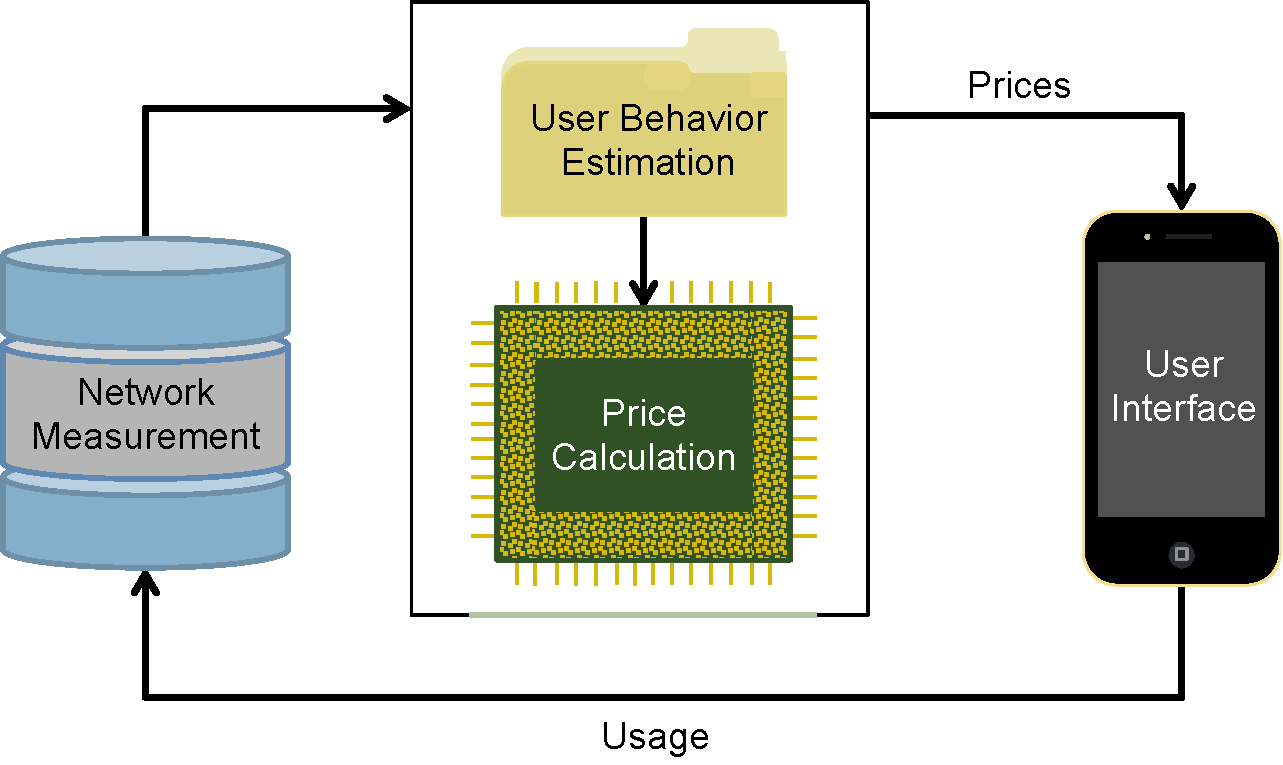
\includegraphics[width = 0.6\textwidth]{Figures/Loop_TUBE.pdf}
\vspace{-0.1in}
\caption{Feedback loop schematic of day-ahead pricing.}
\label{fig:tube-loop}
% \vspace{-0.05in}
\end{figure}

\textbf{\emph{Day-ahead time-dependent:}} In an effort to increase user certainty of the prices, ISPs can guarantee their time-dependent prices one day in advance, and continue to compute new prices to maintain this sliding one-day window of known prices \cite{ha2012tube,Carlee}. Users can then plan their usage in advance, while ISPs can adapt their estimates of user behavior and usage volume in calculating the prices for subsequent days. Day-ahead pricing thus strikes a balance between user convenience and ISP adaptability. This has been a successful pricing mechanism in the electricity market, and hence can be adapted to broadband networks with careful consideration. A schematic of the resulting feedback loop is shown in Figure \ref{fig:tube-loop}. In the next section, we examine a prototype of day-ahead pricing for mobile data in order to illustrate the ``end-to-end'' nature of an SDP deployment.

We pause to briefly compare day-ahead TDP with the other types of dynamic pricing discussed above. Real-time pricing and Smart Market mechanisms require users to delegate some control and operate in an automated mode as the time-scale is too short for user-mediated choices. On the other hand, simple 2-period (day \& night) time-of-day pricing has time scale that is too long to take advantage of any spare capacity availability and time elasticity of demand which vary at much shorter time-scale. Auction-based mechanisms will require modifications to the network equipments (e.g., agents to recognize bid amounts and perform admission control) and client side agents for automated bidding. Raffle-based pricing creates uncertainty in rewards and unless the time-varying prices are known in advance, users may be reluctant to adopt such data plans. A day-ahead dynamic time-dependent pricing plans solves many of these issues by providing guarantees on the future prices in advance, takes advantage of demand elasticities at shorter time-scales, and provides ISPs with a mechanism to optimize the prices they offer.  

But what are the challenges of realizing dynamic day-ahead time-dependent pricing?
\begin{itemize}
\item How to develop an economic model for dynamic day-ahead TDP which computes optimized prices that accounts for users' time elasticity of demand in maximizing the total revenue of the network provider? The price computation needs to consider (a) the cost incurred in offering price discounts, (b) savings from shifting some traffic from peak to off-peak hours, (c) the increase in baseline demand in discounted periods due to potential ``sales day" effect.
\item How to engineer a system that enables this pricing by developing both provider and client-side modules (in particular, the user interfaces needed for users to react to the offered prices)?
\item How can researchers carry out field trials of such pricing plans by interposing themselves as a ``bandwidth reseller" between the network providers and its real consumers?
We will address these questions in Sections \ref{sec:dayahead}, \ref{sec:psychology}, \ref{sec:engg}, and \ref{sec:TDP}.  
\end{itemize}

\subsection{Comparison with other Markets: Similarities and Differences }

Let us now take a look at what forms of time-dependent pricing have been already field tested and exist in the real world in networks that suffer from congestion problems to identify differences and opportunities for innovating TDP plans for broadband networks.   
Much like today's data networks, the electricity and transportation markets have both experienced a capacity shortage over the past decade and have developed new pricing plans to cope with the resulting shortfall. By comparing electricity usage and road traffic to data traffic, we see that these industries are quite similar to data networks, and that their pricing plans may inform SDP for mobile data. Indeed, both industries observe a highly variable demand throughout the day, allowing for both static and dynamic pricing plans.
%Over the past decade, the electricity market has experienced a capacity shortage much like that anticipated for wireless ISPs in the near future.  
In particular, time-of-day road tolls have been offered in many transportation networks, and many electricity utilities have both trial-ed and deployed time-of-day pricing. We give an overview of such pricing plans in this section, with the aim of highlighting the unique challenges posed by refining such pricing plans to accommodate broadband data networks. Figure \ref{fig:compare} gives an overview of the analogies between pricing plans proposed for the transportation, broadband, and electricity industries.

The similarities and differences between these pricing plans reflect the different industries for which they are designed. In particular, we observe the following distinctions:
\begin{enumerate}
\item
\textbf{\emph{Real-time communication:}} User devices on data networks, e.g., smartphones, are capable of real-time communication with the ISP network, for instance if the prices change in real time. But such real-time feedback for price (toll) changes in road networks is harder to realize and will require additional infrastructural support. In electricity markets, new smart grid interfaces have been developed that can display real-time prices, but individual devices, e.g., air conditioners or vacuum cleaners, generally cannot interact directly with the provider smart grid and require a smart energy controller to schedule their energy consumption.
\item
\textbf{\emph{Elasticity of demand:}} Smartphones' ability to communicate with the ISP network in real time is complemented by users' ability to easily control their usage on individual devices and applications. For instance, a user could simply stop streaming a video if the price increases; such measures could also be automated within the device. The users' decisions will reflect the large variance in the demand elasticity of different types of applications (some of which, such as software downloading, P2P, file backup may not even require user participation and can be completed in small chunks whenever low prices are available). In contrast, devices on electricity networks typically consume energy constantly as long as they are active. There is little opportunity for many devices (e.g., washer, dryer, lights) to complete their activities in an intermittent manner without requiring active user engagement. In road networks, the contrast is even more stark; users in the network (e.g., already driving) cannot easily exit or postpone their activity.
\item
\textbf{\emph{Long-term volatility:}} Most people do not have a concrete idea of how much data they consume each month, partly because most data plans charged a flat fee for unlimited access until recently. Moreover, an individual's data usage can vary greatly from day to day, as relatively casual actions such as streaming a video can have a large impact on total data consumption. In contrast, most people have a relatively good idea of how much they drive per day, and the distance traveled, and road toll fees. Thus, people may be more able to plan ahead by buying permits (e.g., EZ pass) or carpooling during congested hours. In electricity markets, household demand similarly does not vary much from day to day. Consumption of electricity is largely driven by user \emph{needs}, rather than the more volatile \emph{preferences} that drive demand for Internet data.
\end{enumerate}
% For instance, user devices on data networks, such as smartphones, are capable of real-time communication with the ISP network, and allow a user to interact with pricing policies in real time. Moreover, users are able to quickly adjust their behavior, e.g., stopping a video streaming session. With transportation networks, users cannot view real-time price adjustments or leave the network easily once they have begun driving. New smart grid technologies enable some real-time price updates, but these are not nearly as widespread as smartphones. Users can often plan ahead more readily for their transportation and electricity needs, e.g., buying permits from secondary markets at congested times. A user's data rate, however, is highly variable even on a long timescale, and most users are not aware of how much data they actually consume. Most people, however, do have an idea of how many miles they drive at what times of the day, which makes planning for road pricing particularly easy.
\begin{figure}
\centering
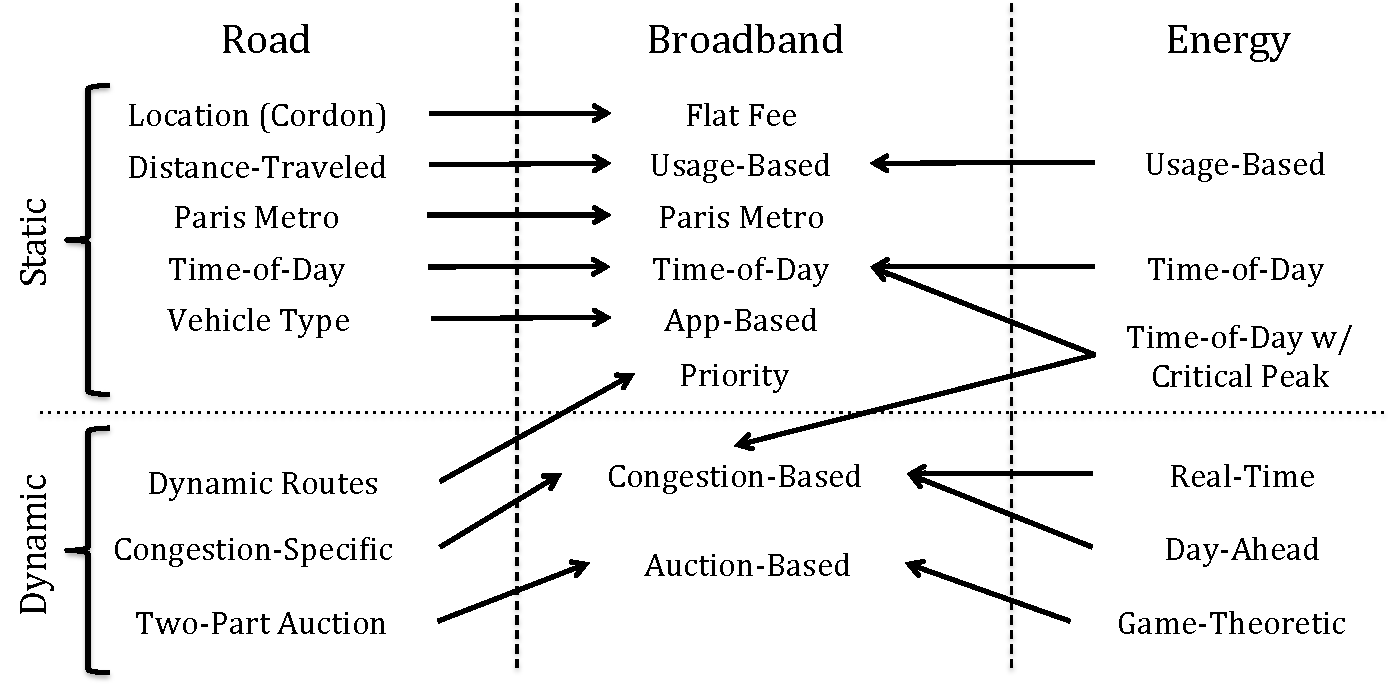
\includegraphics[width = 0.6\textwidth]{Figures/Relationships.pdf}
\caption{Comparison of pricing plans in the transportation, broadband, and electricity industries.}
\label{fig:compare}
\end{figure}
% These trials and the accompanying literature suggest that similar plans may be adopted by network operators. 
% Indeed, the electricity and broadband networks are quite similar in that data traffic can be compared to electricity usage, while different data applications are analogous to different energy-consuming household appliances.  In light of this analogy, the discussion below gives a brief overview of the existing literature on pricing for electricity industries, focusing on time-of-day and dynamic pricing.  A summary of all these pricing policies and their related literature is provided in Table \ref{references}.


\subsubsection{Static Pricing}

Traditional road pricing has been simple flat-rate cordon pricing, analogous to flat pricing of data. Pricing by vehicle type, analogous to app-based pricing for data, has also been proposed, e.g., charging trucks more than passenger vehicles \cite{ushighways}. Forms of flat-rate priority pricing have also been implemented, most obviously in the Paris metro's pricing scheme from which data networks' Paris metro pricing takes its name. High-occupancy vehicle or ``carpool'' lanes can also been seen as analogous to priority pricing, in that users can self-select to take advantage of less-congested HOV lanes by paying the higher ``price'' of carpooling with other passengers.

In a common variation on flat-rate tolls in road networks, the flat-rate toll can vary depending on the time of the day \cite{RoadPricing}, for a pricing plan analogous to time-of-day pricing. However, such charges are still flat-rate, i.e., they do not depend on the distance traveled over the road network. Distance-traveled pricing, analogous to usage-based pricing in broadband networks in that users' charge is proportional to the distance traveled, has also been proposed for transportation networks, and has been offered in Taiwan and the U.S. \cite{holguin2006comparative,wen2005traveler}. In fact, the Taiwanese implementation varies the distance-traveled price depending on the time of the day; it is thus a form of time-of-day pricing.

Time-of-day pricing is the major form of static pricing practiced in the electricity industry. Most trials of time-of-day pricing for electricity markets have focused on peak/off-peak pricing, as electricity demand generally follows a less variable pattern than data demand, with extremely low demand at night and higher demand during the day. For instance, one major source of electricity consumption is air conditioning in the summer, which follows a fairly regular pattern of being on during the day and off at night. Indeed, many trials have shown time-of-day pricing to be effective in reducing excess demand during peak hours. One popular variant that has also been trial-ed is \emph{critical peak pricing}, in which certain days are designated as ``critical,'' e.g., especially hot days during the summer. On these critical days, the peak price goes up to increase users' incentives to reduce demand. Some studies with California consumers have shown that critical-peak pricing is much more effective than simple peak/off-peak pricing \cite{CharlesRiver,herter2007residential}. In this trial, users with ``smart devices'' that automatically reduce energy consumption reduced their usage almost twice as much as other users, indicating that user interfaces for interacting with prices are critical to the success of dynamic or time-of-day pricing plans.

\subsubsection{Dynamic Pricing}

Congestion-based pricing has been proposed in both the transportation and electricity industries. One form of congestion pricing in road networks charges users at a price-per-mile rate that is based on their average speed. However, though considered in Cambridge, U.K., this pricing plan was never implemented \cite{RoadPricing}. A more complex pricing plan proposed using several dynamic origin-destination models to compute effective route costs depending on real-time congestion conditions in the road network \cite{Joksimovic}. Drivers would then be able to take shorter routes for higher prices; however, computing these prices is highly non-trivial, and it would be difficult to communicate the prices of different routes to drivers in the network.

One variation on dynamic pricing for road networks involves a \emph{secondary market}, in which governments can sell permits to pass through congested areas. Users can then form a market to sell these permits \cite{starkie1986efficient}. However, similar pricing schemes have not yet been proposed for data networks, likely due to the difficulty in setting up a secondary market among users. Moreover, the increasingly ubiquitous nature of data connectivity has made it more impractical to ask users to completely refrain from consuming data at congested times.

Some electricity pricing researchers have argued that dynamic pricing can lead to significant gains over simple ToD pricing \cite{borenstein2005long}. Both congestion pricing and auction pricing have been proposed for electricity markets; however, such works often have a more consumer-focused outlook than do pricing proposals for data.
%
In an auction-based electricity market, electricity distributors can make dynamic offers to users (i.e., households) who respond with real-time electricity purchases.  Auction schemes have been proposed that take into account varying electricity capacity, which can significantly improve market efficiency \cite{vytelingum2010trading}.

Many papers have studied responsive dynamic pricing from a user's perspective of predicting future prices and scheduling devices accordingly.  A game-theoretic framework can be used to model users' scheduling of energy usage as a cooperative game; if users cooperate, the total demand on a network can then be reduced, enhancing efficiency \cite{caron2010incentive}. Other works propose algorithms to predict prices in advance \cite{Du,mohsenian2010optimalres} and schedule user devices accordingly; users thus try to anticipate electricity providers' real-time pricing. This price prediction is not necessary with day-ahead pricing, though day-ahead pricing offers electricity providers less flexibility \cite{joe2012optimized}. However, such prediction and scheduling algorithms, which have received relatively little attention for data usage, might help make dynamic congestion pricing for data more amenable to users.

% Mohsenian-Rad et. al.'s related paper \citeyear{mohsenian2010optimal} considers the same problem, but with an emphasis on several users sharing a power source and simultaneously scheduling energy consumption in a distributed manner.  More recently, Du and Lu \citeyear{Du} introduced an appliance commitment algorithm that schedules thermostatically controlled household loads based on price and consumption forecasts to meet an optimization objective.

Other papers consider users' actions in conjunction with the provider's price determination \cite{borenstein2002dynamic}. Such approaches can facilitate a study of social welfare, and may incorporate uncertainty in supply and demand \cite{brunekreeft2000price,chao1983peak,samadi2010optimal}. One may also consider a feedback loop between users and an electricity provider, which can yield real-time pricing algorithms analogous to those for dynamic congestion control in data networks \cite{roozbehani2010dynamic}.
Some works have also considered appliance-specific models of user demand, analogous to different applications having different demands for data \cite{li2011optimal}. A unique feature of these models is the ability to store electricity, e.g., in batteries, for use in later congested periods. Thus, from the provider's perspective, the user can effectively shift his or her energy consumption to less congested times, even though from the user's perspective nothing has been shifted.

\section{Economics of SDP}\label{sec:econ}

% The main goal of smart data pricing is to relieve network congestion by incentivizing users to alter their behavior. Using pricing as an incentive mechanism is not a new idea--indeed, it might be said that most pricing plans exist to incentivize users! Regarding mobile data usage specifically, one can divide the prior literature into two categories: \emph{static pricing}, in which the offered prices are essentially fixed and change on a timescale of months or years, and \emph{dynamic pricing}, in which the prices offered change on a timescale of seconds or hours. In this chapter, we use one example of static and one example of dynamic pricing to elucidate key economic concepts useful for smart data pricing research.

Given the wide variety of SDP pricing algorithms presented in Section \ref{sec:congestion}, a thorough discussion of the theory behind each one is impractical for a book chapter. In this section, we instead select four representative scenarios to illustrate some of the key economic principles often used in formulating different types of pricing algorithms. We first consider static pricing on a single link, and then consider both real-time dynamic pricing and day-ahead time-dependent pricing. Readers familiar with network economics may wish to skip this section.

\subsection{Usage-Based Pricing: A Single Link Example}\label{sec:single}

An operator generally sets its mobile data prices so as to achieve a certain objective, e.g., maximizing profit. In this section, we review some standard economic concepts that are often used in formulating such objective functions. We consider two agents: end users and ISPs.\footnote{Sponsored content and app-based pricing models may also include content providers as a separate type of agent.} For simplicity, we consider only one ISP with a given set of customers, and we suppose that the ISP wishes to build a last-mile access link in its network. The ISP wishes to determine both the \emph{capacity to provision} on this link, as well as the \emph{price per unit bandwidth} to charge its users on the link. This is a standard monopolist profit maximization that we discuss below. We denote the capacity with the variable $x$, and the price by the variable $p$. The ISP-user interaction is summarized in Figure \ref{fig:supply-demand}.

\begin{figure}
\centering
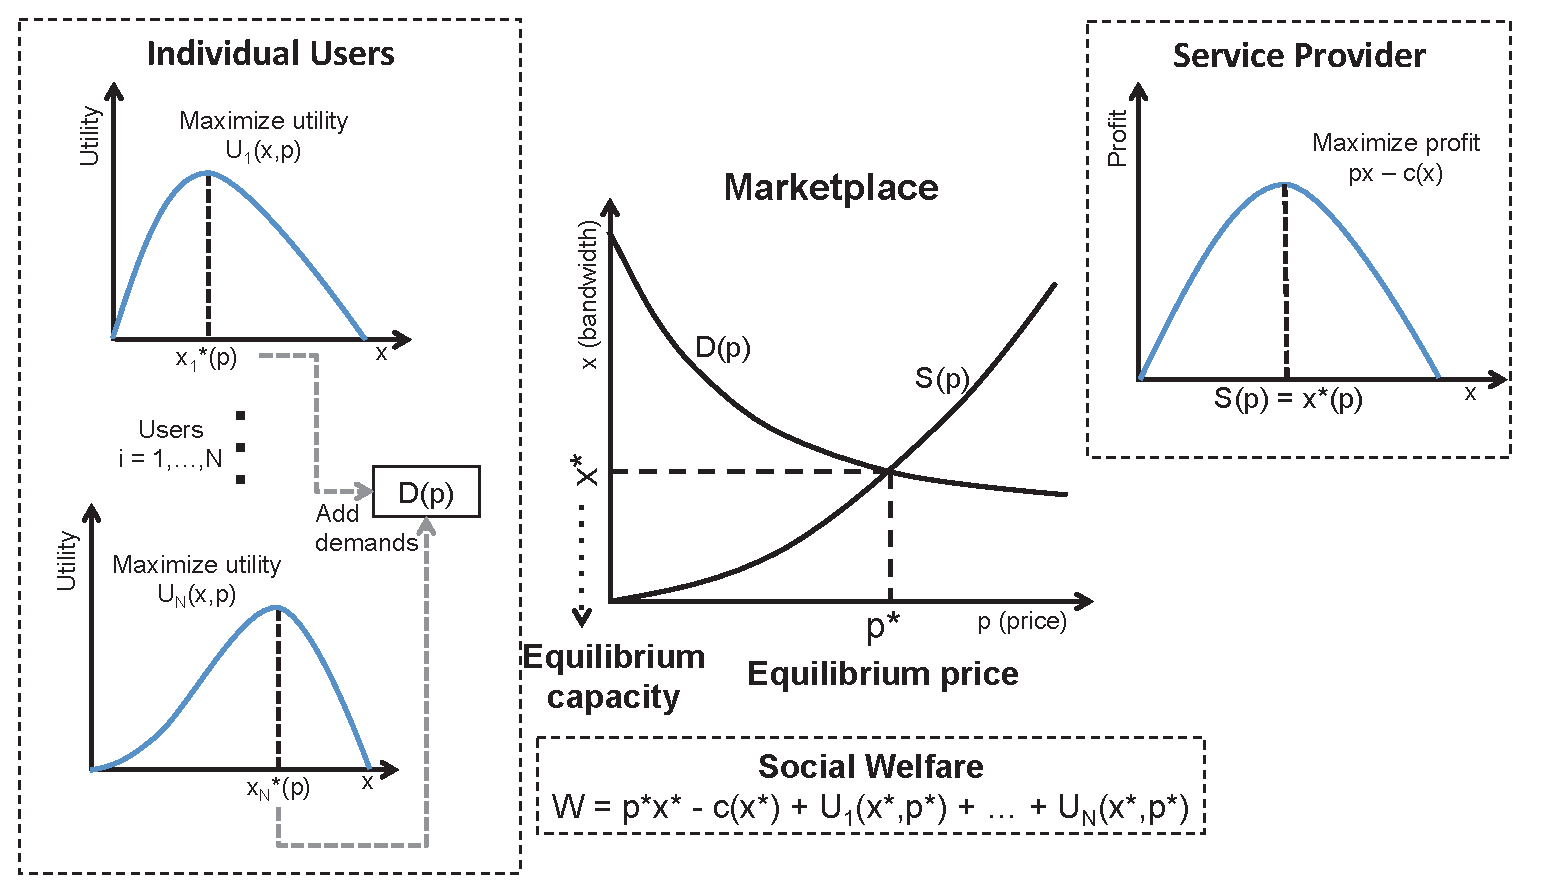
\includegraphics[width = 0.8\textwidth]{Figures/Supply_Demand.eps}
\caption{User-ISP interaction in a mobile data marketplace.}
\label{fig:supply-demand}
\end{figure}

We first consider users' decisions to purchase certain amounts of bandwidth on the ISP's new access link. In modeling this user behavior, we suppose that each user acts so as to maximize his or her \emph{consumer surplus function}, denoted by $U_j(x_j,p)$ for each customer $j = 1,2,\ldots, J$. The function $U_j$ is the net benefit to a consumer from the utility received in purchasing $x_j$ amount of bandwidth for a price $p$ per unit bandwidth.\footnote{This function may be additively decomposed into the form $U_j(x_j,p) = V_j(x_j) - px_j$, i.e., a utility term $V_j$ and the price paid $px_j$. In this scenario, $V_j(x_j)$ is often called the utility, and $U_j(x_j,p)$ the net benefit received by the user. Additively incorporating the price can also be interpreted as incorporating user budget constraints through Lagrange multipliers; more details can be found in Section \ref{sec:realtime}.} Thus, given a price $p$, if $U_j(y_j, p) > U_j(x_j,p)$, user $j$ prefers to purchase $y_j$ units of bandwidth, rather than $x_j$ units. Since the ISP chooses the value of $p$, each user $j$ takes the price as given and chooses the quantity of bandwidth to purchase $\left(x_j\right)$ so as to maximize the utility $U_j(x_j, p)$. We denote this utility-maximizing quantity as $x_j^\ast(p)$.\footnote{The argument $p$ emphasizes the fact that this optimal bandwidth $x_j^\ast$ depends on the price $p$ offered by the ISP.} These functions $x_j^\ast(p)$ are called users' \emph{demand functions}; adding them up, we obtain the \emph{aggregate demand function}, $D(p) = \sum_j x_j^\ast(p)$.

We now consider the ISP's problem of choosing a link capacity $x$ and price $p$. Given a price $p$ and assuming full utilization of the link capacity, the ISP chooses $x$ so as to maximize its utility function. Usually, the ISP's utility is simply its \emph{profit}, but other functions can be used. We write the ISP profit as $px - c(x)$, where $px$ is the ISP revenue and the function $c(x)$ denotes the cost of building a link of capacity $x$. Given $p$, the ISP can then find $x^\ast(p)$, the optimal link capacity as a function of the price $p$. We use $S(p) = x^\ast(p)$ to denote this supply side function.

When the user and ISP are at a \emph{market equilibrium}, supply equals demand: $D(p) = S(p)$. At such a price $p^\ast$ satisfying this relation, each user maximizes his or her own utility by purchasing $x_j^\ast\left(p^\ast\right)$ amount of bandwidth, and the ISP maximizes its utility by providing just enough capacity $x^\ast\left(p^\ast\right) = \sum_j x_j^\ast\left(p^\ast\right)$ to support those users' demands.
%
One often-analyzed property of this equilibrium is the \emph{social welfare}, defined as the sum of the utility received by all users $j$ and the ISP:
\begin{equation*}
\sum_j U_j\left(x_j^\ast,p^\ast\right) + p^\ast\sum_j x_j^\ast\ - c\left(\sum_j x_j^\ast\right),
\end{equation*}
where $x_j^\ast$ is understood to be evaluated at the equilibrium price $p^\ast$. This social welfare can be divided into two portions: the \emph{user surplus}, or the sum of user utilities, and the \emph{ISP surplus}, or the utility (here, profit) obtained by the ISP. Depending on the utility functions $U_j$ and the cost function $c$, the total social welfare may change, and the users and ISP may receive different portions of the overall social welfare.

Before moving on, we pause to discuss some of the more common extensions of the simple problem above. One is to introduce \emph{budget constraints} on each user's utility maximization problem: the user may not want to spend more than a certain amount $B_j$, in which case each user $j$ maximizes the utility $U_j(x_j,p)$ subject to the constraint $px_j \leq B_j$. We may also consider a situation in which users impose \emph{externalities} on each other, i.e., a given user $j$'s utility is affected by the capacity allocated to other users $i\neq j$. For instance, there may be a positive externality in which user $j$'s utility increases as other users send traffic over the link in order to interact with user $j$. On the other hand, one could also observe negative externalities, in which congestion from other users' traffic diminishes a particular user's utility, e.g., by increasing delay.

When solving for the market equilibrium above, we initially took the price $p$ as fixed for the end users and ISP, and then found the equilibrium market price $p^\ast$. In fact, one can obtain this equilibrium price by only examining the optimal behavior of end users and ISPs, i.e., without explicitly considering market equilibrium. Suppose that the ISP, knowing users' demand functions $x_j^\ast(p)$, calculates its revenue as a function of price to be $p\sum x_j^\ast(p)$ (the price, multiplied by the user demand as a function of price). The ISP can then choose both $p$ and $x$ so as to maximize its profit $p\sum_j x_j^\ast(p) - c(x)$, subject to the constraint that the link capacity be able to accommodate users' total demand $\sum_j x_j^\ast$, i.e., that $x \geq \sum_j x_j^\ast$. It is easy to see that (assuming the cost $c(x)$ is increasing in the capacity $x$), at the optimum, $x = \sum_j x_j^\ast$. The ISP then chooses the optimal price $p$ so as to maximize $p\sum_j x_j^\ast(p) - c\left(\sum_j x_j^\ast(p)\right)$. One can show that the resulting optimal price, which we will call $\overline{p}$, is the same equilibrium price $p^\ast$ obtained above: at $\overline{p}$, each user $j$ demands $x_j^\ast(\overline{p})$, and the ISP chooses its optimal capacity $x^\ast(\overline{p})$. This is exactly the point at which the supply and demand curves intersect, i.e., $p^\ast$.

The above reasoning, in which an ISP chooses a price to offer subject to users' behavior as a function of the price chosen, is a simple example of a \emph{game} between users and ISPs. In such a game, several players interact with each other, and each player acts to maximize his or her own utility, which may be influenced by other players' decisions. For instance, in this scenario, users interact with the ISP by utilizing the access link in its network and paying some price. Their decisions on how much capacity to utilize (i.e., choosing $x_j^\ast$) are influenced by the ISP's choice of the price $p$. This interpretation of the single-link example leads us to next consider some basic principles of \emph{game theory} in relation to SDP.

\subsection{Incentive Compatibility: Game-Theoretic Principles}\label{sec:gametheory}

To illustrate some of the basics of game theory, we again consider the single link example above. The user-ISP interaction in such a scenario is an example of a \emph{Stackelberg game}, in which one player, the ``leader,'' makes a decision (e.g., the ISP sets a unit price $p$ for link capacity) and the remaining players, or ``followers,'' then make their own decisions based on the leader's actions. In SDP, this framework reflects the need to consider users' and ISPs' optimal actions when choosing pricing policies that incentivize particular types of resource allocations. In this example, users choose their demands $x_j^\ast(p)$, given the ISP's price $p$. Stackelberg games, which often arise in user-ISP interactions, may be solved using \emph{backwards induction}: first, one computes the followers' actions as a function of the leader's decision (in our example, we compute the functions $x_j^\ast(p)$). The followers' actions are sometimes called a \emph{best response} to the leader. The leader then takes these actions into account and makes his or her own decision (given that users' demands are $x_j^\ast(p)$, the ISP chooses the optimal price $p$). This decision is then the best response to the followers.

The backwards induction process leads to a \emph{subgame perfect equilibrium} in the Stackelberg game: at this equilibrium, each player is maximizing his or her own utility, and no player has an incentive to change his or her behavior. To formalize this definition, we will need to first explain the concept of a \emph{Nash equilibrium}. Consider a general game with $n$ users, each of whom can take an action, e.g., by choosing the value of a variable $y_j$; $j = 1,2,\ldots,n$; and suppose that each user $j$'s utility $V_j$ is a function of all of the $y_j$ variables, i.e., $V_j = V_j\left(y_1,y_2,\ldots,y_n\right)$. Then a set of actions $z_1,\ldots,z_n$ is a Nash equilibrium if $V_j\left(z_1,\ldots,z_j,\ldots,z_n\right) \geq V_j\left(z_1,\ldots,y_j,\ldots,z_n\right)$ for any $y_j \neq z_j$. In other words, assuming that all the other players take actions $z_i$, player $j$'s action $z_j$ optimizes its utility $V_j$.

We may generalize the concept of a Nash equilibrium to a Stackelberg game's subgame-perfect equilibrium by considering \emph{subgames} of the Stackelberg game. We do not give the general definition of a subgame here, but it may be understood by envisioning the Stackelberg game as a dynamic game with different levels defined by the time of decision: on the first level, users make their decisions, and on the second, ISPs make their decisions. A subgame encompasses a group of players who mutually interact, but do not directly interact with other players at their level. In our scenario, a subgame would be a subset of users and the ISP. A subgame-perfect equilibrium of the full Stackelberg game is then a set of actions that comprise a Nash equilibrium in each subgame of the full game. It can be shown that any equilibrium found from backwards induction is a subgame-perfect equilibrium; one can easily check that this is the case in our example scenario. Nash and subgame-perfect equilibria are considered stable in that once they have been achieved, no user has an incentive to change their behavior. (Unfortunately, one cannot in general guarantee that such an equilibrium will be achieved in the first place, and a game may have multiple Nash equilibria.)

Another type of game that often arises in SDP is that of competing service providers. For instance, we may have an \emph{oligopoly} of a few companies who dominate the market for mobile data, e.g., AT\&T and Verizon in the United States are the dominant market players. Each of these companies then competes for customers (i.e., market share) and revenue with the others. This competition defines their interactions, and each company can try to make strategic decisions that optimize its market share. Given a mathematical model of the companies' actions, one can then try to study the corresponding game, e.g., by computing possible Nash equilibria.

While certainly useful for explicit pricing problems like that considered above, game theory can also be applied to more general resource allocation problems, just as SDP allows ISPs to incentivize users to consume data so as to realize particular resource allocations. To illustrate these uses, we again consider the single link example, but we now suppose that the link's capacity is fixed and that the ISP wishes to allocate this fixed amount of capacity $x$ among its $n$ users.

If users selfishly maximize their individual utilities (i.e., choose demands $x_j^\ast(p)$), then the ISP can set a virtual price $p$ to force an allocation in which $\sum_j x_j^\ast(p) = x$, i.e., all of the available capacity is utilized, and each user maximizes his or her utility. This price serves as a signal through which the ISP can control users' demands. However, such an allocation may be unfair: very price-sensitive users may be able to afford significantly less capacity than others. Since revenue is no longer involved, the ISP can afford to care about other objectives like fairness. Indeed, a vast literature exists on just such a problem; we will not go into fairness theory here, but we will present one approach inspired by game theory.

In the Stackelberg game discussed above, users did not cooperate: each user maximized only his or her own utility, subject to the ISP's offered price. Yet if users do cooperate, they may reach a better decision. We can study this problem by first defining individual users' utilities $U_j(y_j)$; given a capacity amount $y_j$, each user $j$ derives utility $U_j(y_j)$. For instance, users could jointly choose their demands $y_j$, subject to the capacity constraint $\sum_j y_j \leq x$, so as to maximize an overall utility function $U\left(U_1(y_1),\ldots,U_n(y_n)\right)$. Depending on the choice of $U$, of course, one would obtain different allocations $y_j^\ast$. We use $y_j^\ast$ to denote the $y_j$ that jointly maximize $U$. Nash proposed that the $y_j^\ast$ satisfy the following four axioms:
\begin{enumerate}
\item
\emph{Invariant to affine transformations:} For each user $j$, define the utility function $V_j(y_j) = \alpha_j U_j(y_j) + \beta_j$ for some constants $\alpha_j > 0$, $\beta_j$. Then the allocation $\left\{z_j^\ast\right\}$ maximizing $U\left(V_1(z_1),\ldots,V_n(z_j)\right)$ satisfies $V_j\left(z_j^\ast\right) = \alpha_jU_j\left(y_j^\ast\right) + \beta_j$ for each user $j$, where the allocation $\left\{y_j^\ast\right\}$ maximizes $U\left(U_1(y_1),\ldots,U_n(y_n)\right)$. An affine transformation of the utility functions $U_j$ does not change the utility received at the optimal allocation.
\item
\emph{Pareto-optimality:} An allocation $\left\{y_1^\ast,\ldots,y_n^\ast\right\}$ is Pareto-optimal if for any user $j$, any feasible allocation $\left\{z_1,\ldots,z_n\right\}$ with $U_j(z_j) > U_j\left(y_j^\ast\right)$ satisfies $U_i(z_i) < U_i\left(y_i^\ast\right)$ for some user $i$. In other words, no user can be made better off without making another worse off.
\item
\emph{Independence of irrelevant alternatives:} Suppose that $U\left(U_1(y_1),\ldots,U_n(y_n)\right) > U\left(U_1(z_1),\ldots,U_n(z_n)\right)$ for two feasible allocations $\left\{y_j\right\}$ and $\left\{z_j\right\}$. Then if the problem constraints are relaxed to allow new feasible allocations, we still have $U\left(U_1(y_1),\ldots,U_n(y_n)\right) > U\left(U_1(z_1),\ldots,U_n(z_n)\right)$.
\item
\emph{Symmetry:} Suppose that $\left\{y_1,\ldots,y_n\right\}$ and $\left\{z_1,\ldots,z_n\right\}$ are feasible capacity allocations with $U_{j_1}(y_{j_1}) = U_{j_2}(z_{j_2})$ for some users $j_1$ and $j_2$, $U_{j_2}(y_{j_2}) = U_{j_1}(z_{j_1})$, and $U_j(y_j) = U_j(z_j)$ for all $j\neq j_1, j_2$. Then $U\left(U_1(y_1),\ldots,U_n(y_n)\right) = U\left(U_1(z_1),\ldots,U_n(z_n)\right)$. In other words, switching the order of the utilities received does not change the overall utility $U$.
\end{enumerate}
An allocation satisfying these four axioms is said to be a \emph{Nash bargaining solution}. One can show that if $U$ is taken to be $\prod_j U_j(y_j)$, then the resulting $y_j^\ast$ is a Nash bargaining solution. Taking the logarithm, we see that this is equivalent to maximizing $\sum_j \log\left(U_j(y_j)\right)$. In other words, users choose their demands to maximize the sum of the \emph{logarithms} of their utilities $U_j$. Since the logarithm is sub-linear for large $U_j(y_j)$, the optimal allocation $\left\{y_j^\ast\right\}$ will penalize large values of $U_j$ relative to smaller ones, yielding a ``more equal'' allocation $U_j\left(y_j^\ast\right)$ than simply maximizing the sum of utilities $\sum_j U_j(y_j)$.

% One way to perform this allocation is to use \emph{virtual prices}, in which the ISP offers a price $p$, just as in our example above. However, the prices are not monetary ones; users do not need to actually pay the ISP. The prices are simply a way for the ISP to (indirectly) allocate capacity to users. simply to impose the requirement that users' total demand equal the capacity $x$. Using the same utility functions $U_j$ and demands $x_j^\ast$ from before, we have $\sum_j x_j^\ast(p) = x$, which may be solved for the optimal price $p$. Yet such an allocation may be unfair: very price-sensitive users may be able to afford significantly less capacity than others. Thus, if an ISP wishes to \emph{directly} allocate 

\subsection{Real-Time Dynamic Pricing}\label{sec:realtime}

So far, we have focused on pricing and bandwidth allocation of a single access link. However, in reality an ISP's network does not consist of single bandwidth links: it is, in fact, a network, with multiple nodes and links between them. Data traffic between two nodes, e.g., between a user and a content provider, flows across a subset of the network links. Since different links may experience different types of congestion at different times, an ISP may want to adjust the prices charged based on how much congestion is experienced by a particular user at a given time. It is this philosophy that lies behind dynamic pricing for congestion control.

To illustrate the basic concepts of congestion control, we consider a relatively simple example given in Kelly et al.'s seminal paper on the subject \cite{kelly1998rate}. Consider a set of nodes, indexed by $n = 1,2,\ldots,N$, and a set of links indexed by $l = 1,2,\ldots,L$ that connect different nodes together. We suppose that each node $n$ wishes to communicate with another node, and we use $R_n$ to denote the subset of links traversed by node $n$'s traffic.\footnote{Choosing the optimal routes for each node $n$ is a non-trivial problem in itself; for simplicity, we assume here that all of the routes $R_n$ are fixed.} The ISP's goal is then to set a traffic rate $x_n$ for each node $n$, such that 1) the total amount of traffic on any link $l$ lies below link $l$'s capacity $c_l$, and 2) all users are as satisfied as possible. To accomplish this, each link can set a unit \emph{congestion price} for traffic on the link. By prescribing the evolution of these prices in time, the ISP can satisfy its two objectives in a distributed manner.

We first define a \emph{routing matrix} to summarize the routes taken by different nodes' traffic over the network: let $R$ be an $L\times N$ matrix, and set $R_{ln} = 1$ if $l\in R_n$, i.e., node $n$'s traffic travels over link $l$, and $R_{ln} = 0$ otherwise. If we concatenate nodes' traffic rates $x_n$ into an $N\times 1$ vector $\vec{x}$, we see that $\vec{y} = R\vec{x}$ yields a vector of length $L$. Each entry $y_l$ of $\vec{y}$ equals the total volume of traffic on link $l$. Letting $\vec{c}$ be an $L\times 1$ vector of the capacities of each link $l$, we then have the capacity constraint $R\vec{x} \leq \vec{c}$: the total amount of traffic on each link $l$ cannot exceed the link's capacity.\footnote{This inequality is to be interpreted component-wise, i.e., each component of the left-hand and right-hand side vectors should satisfy it.} This constraint ensures that the ISP's first objective is satisfied.

The ISP's second objective is that each user be ``as satisfied as possible.'' We define satisfaction by defining utility functions $U_n(x_n)$ for each node $n$; the ISP is then assumed to assign source rates $x_n$ so as to maximize the total sum of utilities, $\sum_n U_n(x_n)$, subject to the constraint $R\vec{x} \leq \vec{c}$. To solve this problem, we next make the assumption that each utility function $U_n$ is concave. Such an assumption is consistent with the economic principle of \emph{diminishing marginal utility}, i.e., that the extra utility received from an additional unit of bandwidth decreases as the user receives more and more bandwidth. Under this assumption, the ISP's objective function $\sum_n U_n(x_n)$ is concave. Since the constraints $R\vec{x}\leq \vec{c}$ are linear, the overall optimization problem is a convex optimization.

We now follow standard optimization theory and introduce a $L\times 1$ vector of Lagrange multipliers $\vec{p}$, with each $p_l$ corresponding to link $l$'s capacity constraint in the component-wise inequality $R\vec{x}\leq \vec{c}$. These multipliers $\vec{p}$ will eventually become the congestion prices set by the links $l$. The ISP's optimization problem is then equivalent to solving
\begin{equation}
\min_{\vec{p}\geq 0}\max_{\vec{x}}\left(\sum_{n = 1}^N U_n(x_n) + \vec{p}^T\left(\vec{c} - R\vec{x}\right)\right).
\label{eq:opt_dyn}
\end{equation}
Solving (\ref{eq:opt_dyn}) centrally can be done relatively easily; it is not hard to see that we have the solution
\begin{equation*}
x_n^\ast = {U_n'}^{-1}\left(q_n\right),\quad p_l^\ast = \begin{cases} 0 &{\rm if}\;c_l - y_l > 0 \\ > 0 &{\rm if} c_l - y_l = 0 \end{cases},
\end{equation*}
where we define $\vec{y} = R\vec{x}$ and the $n$th entry of the $N\times 1$ vector $\vec{q} = R^T\vec{p}$ equals the sum of the congestion prices for the links traversed by node $n$'s prices; $q_n$ thus represents the total price paid by user $n$. However, our goal is to develop a \emph{distributed} solution, in which nodes adjust their rates $x_n$ and links adjust their prices $p_l$ so as to converge to the optimal solution. The ISP can drive these dynamics with the link prices--i.e., links change their prices $p_l$, and nodes respond by adjusting their rates $x_n$ according to the solution above. An example of a price-driven algorithm is \cite{low1999optimization}
\begin{equation}
p_l(t + 1) = \left[p_l(t) - \gamma \left(y_l(t) - c_l\right)\right]^+,\quad x_n(t + 1) = {U_n'}^{-1}\left(q_n(t + 1)\right),
\label{eq:dyn}
\end{equation}
where the argument $t$ denotes the value of a variable at time $t$, and we consider discretized times $t = 1,2,\ldots$ The constant $\gamma > 0$ is a stepsize parameter, and the $+$ superscript $\left[\alpha\right]^+$ denotes the maximum of a quantity $\alpha$ and 0.\footnote{This modification ensures that the prices are nonnegative.} We note that each link $l$ evolves its price $p_l$ using only the traffic on that link $y_l(t)$ and its capacity $c_l$, both of which are known without communicating with other nodes or links. Similarly, each node $n$ adjusts its rate $x_n$ based only its price $q_n$, a quantity that can be carried with node $n$'s traffic and is known without node $n$ communicating with other nodes or links. One can show that these dynamics converge to the optimal prices and rates if the stepsize $\gamma$ is sufficiently small. Moreover, as user utilities $U_j$ or link capacities $c_l$ change over time, following the dynamics (\ref{eq:dyn}) will reposition the rates and prices to their new optimal values. Thus, real-time dynamic pricing can adapt to network congestion levels and keep ISP traffic from exceeding the network capacity. We explore some variations on this dynamic pricing model in the next section.

\subsection{Dynamic Day-ahead Time-Dependent Pricing}\label{sec:dayahead}

One limitation of real-time dynamic pricing is that it requires users to respond to price changes by adjusting their demands in real time. Yet to consciously involve users in adapting their demand to price changes, a longer timescale is preferable.\footnote{There is of course a tradeoff in choosing the timescale: while longer timescales are simpler for users to understand, shorter timescales allow prices to more accurately reflect congestion.} In this section, we again consider the case of a single access link for longer timescale time-dependent pricing. Our goal is to develop an alternative model that is simple enough to be practical as a real pricing plan, yet also helps to alleviate congestion on ISP networks. We aim to offer prices to users in advance, so that users can have more certainty in planning changes to their usage behavior. Indeed, previous studies showed that prices which change in real time can discourage changes in usage, as users are not sure whether the price will decrease in the future \cite{shih2001pricing}. Additionally, in computing the optimized prices (discounts) that maximize network provider's profit, the model needs to consider (a) the cost incurred from offering price discounts, (b) the savings from shifting some traffic from peak to off-peak hours, and (c) the increase in baseline demand in discounted periods due to potential ``sales day" effect.

We divide one day into $T$ time periods--e.g., $T = 24$ periods of one hour each--and suppose that the ISP can offer a different price at each time $t = 1,2,\ldots,T$. We suppose that the ISP has an existing link of capacity $C$, and that it may accommodate additional demand at a marginal rate $\gamma$. This additional cost may represent the increased cost of handling customer complaints once usage exceeds capacity $C$, or an additional investment cost necessary for increasing the network capacity. We let $X_t$, $t = 1,2,\ldots,T$, denote user demand at each time $t$. Then the ISP's cost of accommodating these demands is
\begin{equation}
\sum_{t = 1}^T \gamma\max\left(X_t - C, 0\right).
\label{eq:capacity}
\end{equation}
Given that accommodating demand in the peak periods is more expensive than demand during less-congested periods in which $X_t < C$, the ISP has an incentive to offer lower prices in less-congested periods, thus inducing users to shift some demand into those periods. This is the core idea of time-dependent pricing: by offering lower prices during less congested times, the ISP can even out its demand over the day, resulting in lower capacity costs. Our treatment here follows that in \cite{ha2012tube}.

To formalize this argument, we next need to develop a mathematical model for users' shifting of traffic in response to the prices offered. We let $p_t$ denote the price offered by the ISP at each time $t$. We suppose that the ISP can offer a maximum price that is normalized to 1, e.g., if the ISP currently offers a usage-based price of 1 without time-dependent pricing. We can then define the discount offered at each time $t$ as $d_t = 1 - p_t$. Users' willingness to shift some traffic from one period $t_1$ to another period $t_2$ then depends on the additional discount offered in period $t_2$, i.e., $d_{t_2} - d_{t_1}$. If $d_{t_2} >> d_{t_1}$, then the user will be able to save more money and thus will be more willing to shift his or her traffic.\footnote{One could also consider functions such as the ratio of discounts in the two periods, but $d_{t_2} - d_{t_1}$ has a reasonable interpretation as the amount of money a user can save by shifting traffic.} However, users' willingness to shift their usage does not just depend on the discounts offered: it also depends on the time shifted $t_2 - t_1$. For instance, a user may be very willing to shift some traffic by half an hour, but much less willing to shift his or her usage by more than an hour, even with the same discounts.\footnote{In this section, we suppose that users only delay their traffic, i.e., traffic is shifted only to later, not earlier, times. In practice both types of shifting can occur, but we make the reasonable assumption that it is more natural for users to delay some traffic than it is to anticipate future usage.}

The discounts offered and time shifted are not the only factors determining how willing users are to shift their data traffic: the \emph{type of traffic} also matters. Software downloads, for instance, may be readily delayed by several hours, but users are often much less willing to delay urgent apps like email retrieval. For simplicity, in the following discussion we assume only one type of traffic, but our model can be easily extended to multiple traffic types by adding up the amount of traffic shifted for each traffic class. Considering multiple traffic classes is necessary for ISPs to accurately take user behavior into account: since each user will have some traffic that can be delayed more than other traffic, the fact that we consider the simultaneous behavior of multiple users need not mitigate the need for multiple traffic classes.\footnote{The amount of traffic corresponding to each traffic class can be treated as a model parameter; along with the other model parameters, it can be estimated from observed aggregate usage data.} We use $w(d,t)$ to denote users' probability (i.e., willingness) to delay their traffic by an amount of time $t$, in exchange for an additional discount $d$. We suppose that $w$ is increasing in the discount $d$ and decreasing in time $t$, and that the value of $w$ lies between 0 and 1, so that it may be interpreted as a probability. Many functions $w$ meet these criteria, e.g., the functions
\begin{equation*}
w(d,t) = \frac{\max(d,0)}{\Gamma(t + 1)^\beta},
\end{equation*}
where $\Gamma$ is a normalizing factor and $\beta \geq 0$ is a model parameter that controls the rate at which willingness to shift decreases with the time shifted $t$. For larger values of $\beta$, the willingness to shift decays faster with time, denoting increased impatience.

The general idea behind our model is to use the $w(d,t)$ functions to calculate how much traffic is shifted to different times of the day, relative to a baseline traffic pattern without time-dependent discounts. Our model thus attempts to reflect users' thought processes in looking at a set of future prices and deciding whether to delay their traffic or not. While a more traditional model would use utility functions (cf. Section \ref{sec:single}) to describe users' behavior, user utility functions are difficult to derive from user behavior, since ``utility'' attempts to quantify the relatively vague idea of ``user benefit.'' The probability of shifting traffic, on the other hand, can be calculated directly from observing the amount of traffic shifted in response to discounts offered to users.

Given the functions $w$, the expected amount of traffic shifted from time $t_1$ to time $t_2$ is
\begin{equation*}
w\left(d_{t_2} - d_{t_1}, \left|t_2 - t_1\right|_T\right),
\end{equation*}
where $\left|t_2 - t_1\right|_T$ denotes the number of periods between time $t_2$ and period $t_1$, modulo the number of periods $T$ (e.g., if $t_2 < t_1$, then $\left|t_2 - t_1\right|_T$ is the number of periods between period $t_1$ and period $t_2$ on the next day). Given an initial amount of traffic $Y_t$ in each period $t$, we calculate that $Y_{t_1}w\left(d_{t_2} - d_{t_1}, \left|t_2 - t_1\right|_T\right)$ amount of traffic is shifted from time $t_1$ to time $t_2$. The ISP then loses $\left(d_{t_2} - d_{t_1}\right)Y_{t_1}w\left(d_{t_2} - d_{t_1}, \left|t_2 - t_1\right|_T\right)$ amount of revenue due to the traffic shifted from time $t_1$ to $t_2$. Some additional revenue is lost from the unshifted traffic in each period, for a total revenue loss of
\begin{equation}
\sum_{t = 1}^T \left[Y_td_t + \sum_{s\neq t} Y_s\left(d_t - d_s\right)w\left(d_t - d_s, \left|t - s\right|_T\right)\right].
\label{eq:loss}
\end{equation}
In addition to this revenue loss, offering discounts at some times may induce users to increase their overall usage during those time periods. This increase is independent of any usage shifted from more expensive times and constitutes a psychological ``sales day effect,'' which was observed during time-dependent pricing trials \cite{ha2012tube,sigchi}. It reflects the qualitative insight that user demand increases as the price charged decreases: users see that they are saving money, relative to usage during high-price periods, and are thus encouraged to spend and use more. The larger the discount offered $d_t$, the larger this increase will be. We can model this increase with a power law: given an initial amount of traffic $Y_t$ in period $t$, the amount of traffic after a discount $d_t$ is offered (neglecting any traffic shifted to other periods) is $Y_t\left(1 + d_t\right)^\alpha$ for some positive model parameter $\alpha$. We then have the desirable property that demand does not change if no discount is offered $\left(d_t = 0\right)$; if $\alpha = 0$, the total demand does not depend on the discount at all. The ISP thus earns additional revenue
\begin{equation}
Y_t\left(\left(1 + d_t\right)^\alpha - 1\right)(1 - d_t)
\label{eq:revenue}
\end{equation}
due to this additional demand in period $t$. We can then add the ISP's revenue loss from discounts offered (\ref{eq:loss}), less the revenue gain (\ref{eq:revenue}) from additional traffic, to the ISP's cost of capacity (\ref{eq:capacity}) to obtain the objective function
\begin{equation*}
\sum_{t = 1}^T \left[Y_td_t - Y_t\left(\left(1 + d_t\right)^\alpha - 1\right)(1 - d_t) + \sum_{s\neq t} Y_s\left(d_t - d_s\right)w\left(d_t - d_s, \left|t - s\right|_T\right) + \gamma\max\left(X_t - C,0\right)\right],
\end{equation*}
where the total traffic at each time $t$ is
\begin{equation*}
X_t = Y_t\left(1 + d_t\right)^\alpha + \sum_{s\neq t} Y_s w\left(d_t - d_s, \left|t - s\right|_T\right) - \sum_{s\neq t} Y_t w\left(d_s - d_t, \left|s - t\right|_T\right).
\end{equation*}
The first term represents the increase in traffic due to the discount, while the second is the amount of traffic deferred into period $t$, and the third term the amount of traffic deferred out of period $t$. The ISP then chooses the discounts $d_t$ (equivalently, the prices $p_t = 1 - d_t$) to minimize its objective function. Under reasonable conditions on $\alpha$, $\gamma$, and $w$, this is a convex optimization problem, which may be rapidly solved.

By solving this optimization problem, the ISP can obtain a set of prices for one day; it can then offer day-ahead pricing by running an optimization in each period that determines the optimal discount to offer one day from the current time. Moreover, the ISP can observe the traffic consumed in each period once these discounts are offered. Comparing this data to the traffic observed without discounts, the ISP can estimate the parameters of its user behavior models (i.e., $\alpha$ and $w$ above) from the observed changes in usage, given the prices offered. These estimates can be periodically updated and used to calculate new prices, completing a feedback loop (cf. Figure \ref{fig:tube-loop}) between users and the ISP \cite{ha2012tube}. 

\section{Psychological Aspects of SDP}\label{sec:psychology}
 
Arguably, the foremost factor in realizing a successful data plan is its adoptability by end users. But this depends not only on good economic models and system capabilities, but also on understanding consumer behavior and psychological aspects, and in particular, how client-side interfaces need to be designed to make them effective. These concerns require the networking researchers to interact and work closely with the ongoing efforts in the human-computer interaction (HCI) community. This section covers some of the basic themes emerging from the HCI research on psychology of Internet users.

As early as 2005, HCI researchers introduced networking, particularly user behavior considerations in home networks, as an important aspect of HCI studies \cite{Grinter2005}. In the context of broadband networks, few HCI works have developed human-facing systems to manage network usage.  The \emph{Eden} system \cite{Eden} modified a home router to provide users with an intuitive interface for managing their ``home network experience." The main focus of such home-networking tools has been on designing GUIs to help users understand the physical location of different devices in their home and be able to perform basic administrative functionalities like perform membership management, access control, network monitoring, etc. In a similar vein, the \emph{Homework project} \cite{Mortier2012} modifies the handling of protocols and services at the home router to monitor data usage, prioritize different devices, and monitor other users� data consumption (usually in the context of parental control) in order to reflect the interactive needs of the home. Other studies have focused on understanding the impact of monitoring and sharing bandwidth speed in a wired home network \cite{chetty2011my}. The authors carried out a field trial with 10 households using a visual network probe designed to help educate and empower consumers by making broadband speeds and sources of slow-downs more visible. In a separate work, Chetty et al. \cite{chetty2010s} also carried out a field trial of their \emph{Home Watcher} bandwidth management tool to study the effect of viewing others� bandwidth usage on social dynamics in the household. They showed that when resource contention amongst different household members is made visible, users have better understanding of bandwidth their usage and allocation, revealing new dimensions in household politics. Yet while these works addressed several crucial elements of network intervention (e.g., throttling, capping, parental control) and its related visualization tools, they have been limited to either modifying the network stack within the OS \cite{chetty2010s} or deploying a custom-built access point \cite{Mortier2012}. In contrast, the need today is to focus on understanding the following issues: (a) how economic incentives (i.e., pricing) can impact and modify mobile user behavior, (b) how researchers can carry out field trials (almost seamlessly from an end-user perspective) by interposing between the ISP and its real customers (i.e., participants). 

In the context of mobile networks, \cite{Roto2006} considers the need for mechanisms to help users track their spending on mobile data. This line of research on user interface designs needs more attention to realize more dynamic pricing plans and study user response to such plans. However, realizing such data plans requires assumptions of rational behavior to be realized in practice, i.e., that people perceive the pricing signals and change their behavior. The Berkeley INDEX project \cite{INDEX} in the 1990s for wired Internet suggested that users should be able to view prices and select desired QoS levels (i.e., bandwidth speed), with similar results reported by the M3I project \cite{M3I}. 
Similar field trials on the HCI aspects of time-dependent pricing for mobile data have been reported in \cite{sigchi}, and the main themes emerging from these studies will be discussed below.

Recently, there have been calls to investigate HCI aspects of time-dependent pricing in the context of ecological sustainability and energy consumption \cite{Pierce2012}. Even without economic incentives, good UI designs of energy monitors have been shown to be effective in changing consumer behavior \cite{Froelich2010,Pierce2012}. These investigations have ranged from a large-scale media art installation visualizing energy consumption in an office building, to power strips that change color to show the energy used by individual electrical sockets \cite{Heller2011,Holmes2007}. One of the usual tradeoffs in visualizing energy usage is the use of pictorial versus numerical usage amounts. For instance, the iPhone application \emph{WattBot} allows users to monitor their home energy usage, with colors indicating usage amounts \cite{Petersen2009}. While the colors enabled users to quickly grasp their qualitative energy usage, users also wanted to track their evolving usage behavior by viewing their usage history \cite{Chetty2008}. In addition to the ``manner" of presenting usage data, users expressed concern over the ``convenience" of checking their usage. For instance, researchers testing a desktop widget that showed computer energy efficiency found that users appreciated the inconspicuous, easy-access nature of the widget \cite{Kim2010}. Many of these design insights were incorporated in the client-side UI design of the TDP trial for mobile users reported in \cite{sigchi}. Another key consideration in designing such mobile applications for smarter data plans is that the GUIs need to be account for the form-factor, presentation, and convenience of use on mobile devices and platforms. Incorporating features like parental control and usage history have been found to be desirable to users, even in the TDP paradigm \cite{sigchi,datawiz}.  

The main themes emerging from these research on HCI aspects of networking are that:
\begin{enumerate}
\item Consumers are very concerned about the increasing cost of data plans but are not fully aware of their monthly usage. Therefore mechanisms that help them to better monitor and control their own usage and allocate bandwidth among household members (or in shared data plans for mobile) are perceived to be useful by users. Moreover, given the right economic incentives, many are willing to wait for some form of a feedback signal from the network on the congestion levels and change their behavior, e.g., choose higher QoS service for critical applications in smart market scenarios \cite{M3I}, or wait for discounted periods for non-critical applications in case of time-dependent data plans \cite{sigchi}. This is therefore a promising direction in the evolution of Internet pricing, and follows similar trends in other markets like electricity and transport networks. 
\item The key factor in enabling smart data plans is designing the user interfaces that are effective and understandable to users. Previous research has shown that well-designed user-side applications can not only help users make decisions on deferring usage, but also can become a tool that helps them to self-educate, monitor, and control their usage and spending. Among the features found to be effective as means of communicating useful information to users were color-coding\footnote{While color-coding has been used and appeared effective in several scenarios, care must be taken to provide a secondary signal for persons suffering from color-blindness.} of price/discounts, information indicators (e.g., current price) on the home screen of devices, usage history, recommendations on usage deferrals, etc.
\item Past research also revealed interesting insights on the user psychology of controlling their usage. First, trial participants viewed parental control at the granularity of apps as being useful in managing their usage. Second, they showed a desire to control their usage manually instead of delegating control to an autopilot mode. When coupled with the desire for parental control, we find users want to take charge of their consumption behaviors, for themselves and their families, in ways that require transparency and flexibility. This tradeoff between users' desire for transparency and control will be an important design considerations for enabling smarter data plans.
\item Consumers prefer a certain degree of certainty in the prices, which explains the popularity of flat-rate plans. Therefore for dynamic and smarter data plans to succeed, the time granularity of changes in prices have to be carefully accounted for. Users want to know and have certainty about these prices/discounts in advance, and therefore naive dynamic pricing plans may not work. In particular, real-time pricing that provides price signals based on current congestion levels may demand a higher degree of user engagement (or automation) than users are willing to adopt. Plans that have been explored in energy markets, such as ``day-ahead'' pricing \cite{ha2012tube,sigchi}, therefore may be more acceptable to users.
\item As both networking and HCI address increasingly complex socio-technical ecosystems, e.g., mobile Internet, cloud computing, smart grids, etc., incorporating economic analysis as a part of user behavior studies is important. There is also a need to understand how researchers can create new frameworks for realistic experiments and field trials on the HCI aspects of network economics. Various research ideas have taken different systems approaches, from modifying the network stack within the OS \cite{chetty2010s} to deploying custom-built access points \cite{Mortier2012}, to the TUBE project \cite{ha2012tube} which developed a system for researchers to act as a resale ISP by interposing between ISPs and their customers, and provided these two sides with client-side mobile applications and ISP-side incentive computation modules.  
\end{enumerate}
 
  
% \cite{Roto2006} 	Roto, V., Geisler, R., Kaikkonen, A., Popescu, A. and Vartiainen, E. Data traffic costs and mobile browsing user experience. In Proc. Workshop on Empowering the Mobile Web, in conjunction with WWW 2006.
%\cite{Grinter2005}	Grinter, R.E., Edwards, K. W. and Newman, M. W. The work to make a home network work. In Proc. ECSCW, Springer (2005): pp. 469 � 488.
%\cite{Eden}	Yang, J., Edwards, W. K. and Haslem, D. Eden: Supporting home network management through interactive visual tools. In Proc. UIST, ACM Press (2010): pp. 109 � 118.  
%\cite{Mortier2012} Mortier, R., Rodden, T., Tolmie, P., Lodge, T., Spencer, R., Crabtree, A., Koliousis, A. and Sventek, J. Homework: Putting interaction into the infrastructure. In Proc. UIST, ACM Press (2012): pp. 197� 206.
%\cite{Chetty2011} Chetty, M., Haslem, D., Baird, A., Ofoha, U., Sumner, B. and Grinter, R. Why is my Internet slow?: Making network speeds visible. In Proc. CHI 2011, ACM Press (2011): 1889 � 1898.
%\cite{Chetty2010} Chetty, M., Banks, R., Harper, R., Regan, T., Sellen, A., Gkantsidis, C., Karagiannis, T. and Key, P. Who�s hogging the bandwidth?: The consequences of revealing the invisible in the home. In Proc. CHI 2010, ACM Press (2010): pp. 659 � 668.
%\cite{Pierce2012} Pierce, J. and Paulos, E. Beyond energy monitors: Interaction, energy, and emerging energy systems. In Proc. CHI 2012, ACM Press (2012): 665 � 674.
%\cite{Froelich2010} Froelich, J., Findlater, L. and Landay, J. The design of eco-feedback technology. In Proc. CHI 2010, ACM Press (2010): 1999 � 2008.
%\cite{Heller2011} Heller, F. and Borchers, J. PowerSocket: Towards on-outlet power consumption visualization. In Ext. Abstracts CHI 2011, ACM Press (2011): 1981 � 1986.
%\cite{Holmes2007}Holmes, T. Eco-visualization: Combining art and technology to reduce energy consumption. In Proc. C&C 2007, ACM Press (2007): 153 � 162.
%\cite{Petersen2009} Petersen, D., Steele, J. and Wilkinson, J. WattBot: A residential electricity monitoring and feedback system. In Ext. Abstracts CHI, ACM Press (2009): 2847 � 2852.
%\cite{Chetty2008} Chetty, M., Tran, D. and Grinter, R. Getting to green: Understanding resource consumption in the home. In Proc. UbiComp 2008, ACM Press (2008): 242 � 251.
%\cite{Kim2010} Kim, T., Hong, H. and Magerko, B. Design requirements for ambient display that support sustainable lifestyle. In Proc. DIS 2010, ACM Press (2010): 103 � 112.


\section{Engineering Aspects of SDP}\label{sec:engg}

Following the works of congestion pricing by Kelly, Gibbens, and others \cite{Kelly-eff,gibbens-kelly,kelly1998rate,kelly2000}, researchers have focused on developing the basic idea of pricing bandwidth resources according to congestion marks (i.e., price ``pollution" instead of just volume). Congestion marks on packets can be used as a mechanism to indicate to the end-users or end-systems (or ``agents") that they may need to pay more to avail a certain level of QoS when the network gets congested. A team of researchers, led by Briscoe,\footnote{http://bobbriscoe.net/pubs.html} today are developing these ideas on the accounting architecture, feedback aspects of congestion signaling, incentive compliance, security etc. in conjunction with working groups like WG CONEX in the IETF\footnote{http://datatracker.ietf.org/wg/conex/charter/} that focus on implementation aspects. One such EU collaborative project, the \emph{M3I} (Market Managed Multi-service Internet) has proposed an architecture for market management of the Internet's QoS and demonstrated new business models that it can enable. The core of the QoS problem tackled by the M3I project is to solve the fast control problem to avoid QoS degradation during short-term congestion. In doing so, the M3I architecture requires network providers to deploy ECN (Explicit Congestion Notification) on all routers so that the congestion experienced field in the IP packet header can be set with a probability related to the current network load, allowing prices to adapt to the congestion conditions in the network. The M3I solution can be realized in different ways and in different scenarios, which have been extensively discussed in \cite{M3I}. One solution uses these pricing feedback signals to encourage self-admission control. In effect this is real time pricing (RTP) version of time-of-day pricing. A second solution synthesizes admission control at the network edge from a dynamically priced wholesale service.\footnote{http://bobbriscoe.net/projects/m3i/dissem/cc02/m31\_cc02.pdf} The M3I technology has also implemented several business models over different QoS mechanisms as discussed in \cite{M3I-business}.  In a similar vein, \cite{Chiu2008} has used game-theoretic model to explore the uplink pricing as a way to provide differential pricing to P2P and regular users in a competitive market.

Like M3I, much SDP research realizes the vision of pushing control out of the network into the hands of the end-users. However, giving users more usage control has to be introduced carefully so that the users are not overwhelmed with choices and network providers do not lose revenue. Users typically prefer to have some certainty about their monthly bills and hence as opposed to real-time dynamic pricing, some SDP researchers have looked at day-ahead time-dependent pricing. But day-ahead pricing requires network providers to be able to optimize for the future prices they are willing to offer based on past usage patterns and their prediction of user elasticity of demand for various types of traffic. On the user-side, it requires developing interfaces through which users can provide their feedback to these prices. 

The key subsystems required in realizing the basic feedback-control architecture envisioned in M3I \cite{M3I} and SDP are:
\begin{enumerate}
\item \emph{Tariff Communication} is used to distribute pricing policy to other subsystems. The Price Communication Protocol (aka Tariff Distribution Protocol \cite{protocol}) is a flexible protocol that can use different transport mechanisms like UDP multicast, HTTP and RSVP to distribute tariffs between the ISP's management systems and to customers. 
\item Charging, Authentication, and Accounting module applies the chosen tariff plan to measured usage data for billing purposes.
\item Price Computation calculates optimal prices to offer to the user. In M3I, this price adapts to the real time network load while in SDP the prices are computed in advance to provide guarantees to the user's expenses. 
\item Optimization and Prediction Modules are used by the provider to predict the future congestion levels and estimate the users' patience across different traffic classes at different types of traffic based on the history of traffic volumes and the observed changes to it in reaction to offered prices. The optimization module then computes the optimal prices (or discounts) to offer to the end-users in the SDP architecture.
\item Data Gathering/Usage Metering is used by the provider as inputs to the charging and accounting systems and for price calculation.
\item Mediation is used to aggregate gathered data and do format conversions as needed.
\item Client Scheduler is used in the SDP framework to create an ``autopilot" mode of operation for the end-user which schedules the various types of application traffic based on user's specified delay elasticities and offered future prices so as to minimize user expenses.
\item Charge Reaction allows customers to react to the offered prices which gets fed back into the feedback-control loop between the ISP and its customers. In some scenarios such function is performed by a software agent on the end-user device (e.g., ``autopilot" mode in SDP or the Dynamic Price Handler in M3I), while in others, as in day-ahead TDP, user interfaces need to be provided for users to react to the offered prices.  
\end{enumerate}       

Next we discuss a case study of a particular realization of SDP --dynamic day-ahead time-dependent pricing; the model considerations for it, system architecture, HCI design aspects and results from a field trail.  

\section{Case Study of SDP: A Trial of Day-ahead TDP}\label{sec:TDP}

While pricing algorithms are essential to SDP research, in practice such algorithms must be able to function within an ISP network. In this section, we discuss the design and results of a trial of Section \ref{sec:dayahead}'s day-ahead time-dependent pricing (TDP) to highlight some ways in which implementability concerns can influence the development of pricing algorithms. We examine some important system and user interface design principles that were used in developing the prototype of this system, called TUBE, and finally present some trial results that illustrate how these elements can come together in practice. While some SDP trials have been conducted in the past, e.g., the Berkeley INDEX project in the 1990s \cite{INDEX}, the design of this TUBE pilot trial illustrates the way new factors such as smartphones' computing capabilities affect SDP's feasibility.

%Economic models for and system design for enabling dynamic pricing, such as time-dependent pricing (TDP), smart market auctions, sponsored access. Developing a control-feedback loop between the network core and end-devices (i.e., demand-response). Need for new usage accounting and signaling protocols. User interface design factors for smart pricing. Results from field trials of TDP systems.

\subsection{Model Considerations}

Most forms of dynamic pricing, in which prices must be determined in (near) real-time, require the prices to adapt based on users' behavior. For instance, users' perception of the prices offered may change over time, and demographically distinct user populations may react differently to the same set of prices (e.g., teenagers versus businessmen). Offering dynamic pricing thus requires that the ISP first estimate its users' behavior and then use this to inform its choice of prices. In the case of time-dependent pricing, such estimates are particularly important. The basic philosophy of TDP is that by offering lower prices at less congested times, an ISP incentivizes users to shift some of their usage from more expensive, congested times to less congested times. Users' demand over the day is thus even-ed out, with peak usage decreasing; this decrease in peak usage then reduces ISPs' need to over-provision capacity for their peak demand. While lower prices would effectively encourage users to shift their demand, thus reducing costs, ISPs would also lose a large amount of revenue if the prices were too low. Moreover, users might shift their usage too much, and end up creating a new peak period during the discounted times.

In practice, these estimates of user behavior must take into account the available information that the ISP can collect from its users. For instance, TUBE's TDP algorithms, discussed in Section \ref{sec:dayahead}, use only \emph{aggregate usage data}, that is, the total usage volume on the network at different times, in order to estimate user behavior and calculate the prices. This approach has the following benefits:
\begin{itemize}
\item
\emph{Scalability:} Since only aggregate usage is recorded and used in the algorithms \cite{ha2012tube}, we can scale up the user behavior and price computations to multiple users and multiple applications. The algorithm complexity does not increase with the number of users contributing to the aggregate usage totals.
\item
\emph{User privacy:} The amount of traffic that an individual consumes for different applications can be sensitive information (e.g., unusually large amounts of streaming video might reveal a movie buff). The TUBE algorithm does not consider application-specific usage, so the ISP need not receive or record such sensitive information.
%\item
%\emph{Application-specific modeling must be estimated}: Different mobile applications respond differently to TDP: users may be much more willing to delay a software update, for instance, than to delay watching a video. Since application-specific usage data, however, our algorithm must estimate the delay sensitivity of different application types.
\item
\emph{Utility function estimation:} Utility function estimation is usually a hard problem. When temporal considerations are involved, it can potentially become even more complicated, as the utility of consuming data at any given time depends on the prices offered at all times of the day. %But the TDP approach proposed in \cite{ha2012tube}  we do not employ utility functions in modeling users' reactions to prices.
\item
\emph{Empirical observations:} Instead of using utility functions, we can model users' willingness to shift their demand from one period to another, depending on the time elapsed between these periods and the price difference. Such usage shifts can be directly observed by comparing the amount used at different times and prices, and the model can then adapt as these observed shifts change over time.
\end{itemize}
By following these principles, we develop a scalable price calculation and user behavior estimation algorithm (see Section \ref{sec:dayahead} and \cite{ha2012tube} for details) that can be feasibly deployed in a real system.

\subsection{System Design}

A core feature of SDP, and time-dependent pricing in particular, is that it involves both end users and ISPs. Thus, the system design must have components both on ISP servers and on user devices. Figure 
\ref{fig:tdp_arch} shows this division of functionality and the requisite communication channels between the user device and ISP server. In order to make the system practical, we follow three basic principles:

\begin{figure}
\centering
\includegraphics[width = 0.6\textwidth]{Figures/TDP_Architecture.pdf}
\caption{User-ISP functionality division and feedback communication in time-dependent pricing.}
\label{fig:tdp_arch}
\end{figure}

\begin{itemize}
\item
\emph{Functionality separation:} Users and ISPs have different roles in an SDP system: while users respond to the prices offered, an ISP must set the prices. TUBE utilizes individual user devices to facilitate not only displaying prices to users, but also helping them respond to the prices offered via an \emph{autopilot mode} that automatically schedules apps to lower price periods. Since such computations need not involve the ISP, this functionality is located on users' devices.
\item
\emph{A feedback loop:} In order to successfully adapt prices to user behavior, the ISP needs to monitor usage in its network.\footnote{Such usage monitoring also allows the ISP to calculate the amount spent by individual users.} Thus, users must periodically send their usage to the ISP server. Similarly, the ISP must periodically update the prices displayed on users' devices as new prices are calculated. This mutual communication forms a feedback loop.
\item
\emph{An open API:} An ISP's users may have many different devices with different operating systems--for instance, iOS, Android, and Windows phones and tablets. Each of these devices must therefore communicate with the ISP server. To ensure consistency across different device types, TUBE offers an open API for transmission of usage and prices between the ISP and users.
\end{itemize}

\subsection{User Interfaces}

SDP depends not just on pricing algorithms and system design, but ultimately on \emph{whether users respond to the prices offered}. Thus, careful user interface design is necessary to ensure that users understand the prices being offered and to encourage them to respond accordingly. In some cases, interface design goes beyond displaying prices; users' devices can automatically adjust data usage based on the prices offered and user preferences. TUBE's user interface components can be grouped into three different categories:
\begin{itemize}
\item
\emph{Information displays:} Since TUBE offers day-ahead TDP, the prices for the next day should be displayed to users. But users may also find it helpful to track their spending by viewing how much usage they have consumed in the past. TUBE thus shows users both the price and usage for several past hours, so that users can understand how they usually respond to the prices offered and how this affects their spending on data. TUBE also shows the amount used for the five apps with the highest data usage, so that users can see which applications consume more data. Figure \ref{fig:tube_gui}abc shows some sample screenshots of these features. 
\item
\emph{Out-of-app indicators:} Most users find checking a mobile application too onerous for keeping track of current or future prices. A more convenient way to display the prices is to show a color-coded price indicator on the device home screen to (qualitatively) signal the current price to the user, without requiring any special action on the user's part. Such color-coding can also be helpful for visualizing the future prices within the app, so that users can quickly decide whether to wait for lower prices.
\item
\emph{Automation:} Many users prefer not to manually schedule different applications due to the complications involved in tracking future prices. TUBE thus offers an \emph{autopilot mode} that takes into account users' delay sensitivity for different applications and monthly budget to automatically schedule some apps to lower-price times. The autopilot mode utilizes users' past spending to forecast how much the user will spend over a month. If this amount exceeds a user's monthly budget, delay-tolerant apps can be scheduled to lower-price periods; as users' spending further exceeds their budget, apps with lower delay tolerances will be scheduled to lower-price periods. However, such algorithms need to be optimized so as to be as non-intrusive as possible; in user interviews after the TUBE trial, many trial participants expressed concern over an automated algorithm controlling their data usage \cite{sigchi}. One way to accommodate these concerns is to allow users to override the autopilot scheduling and to configure algorithm parameters, e.g., changing the delay tolerances of different apps (Figure \ref{fig:tube_gui}d).
\end{itemize}
% The current and future prices, as well as corresponding usage volumes, are shown; the prices are color-coded to aid visual comprehension. Users can also schedule apps for future, lower-price times.
\begin{figure}[t]
% \vspace{-0.05in}
\begin{center}
\begin{subfigure}[b]{0.22\textwidth}
	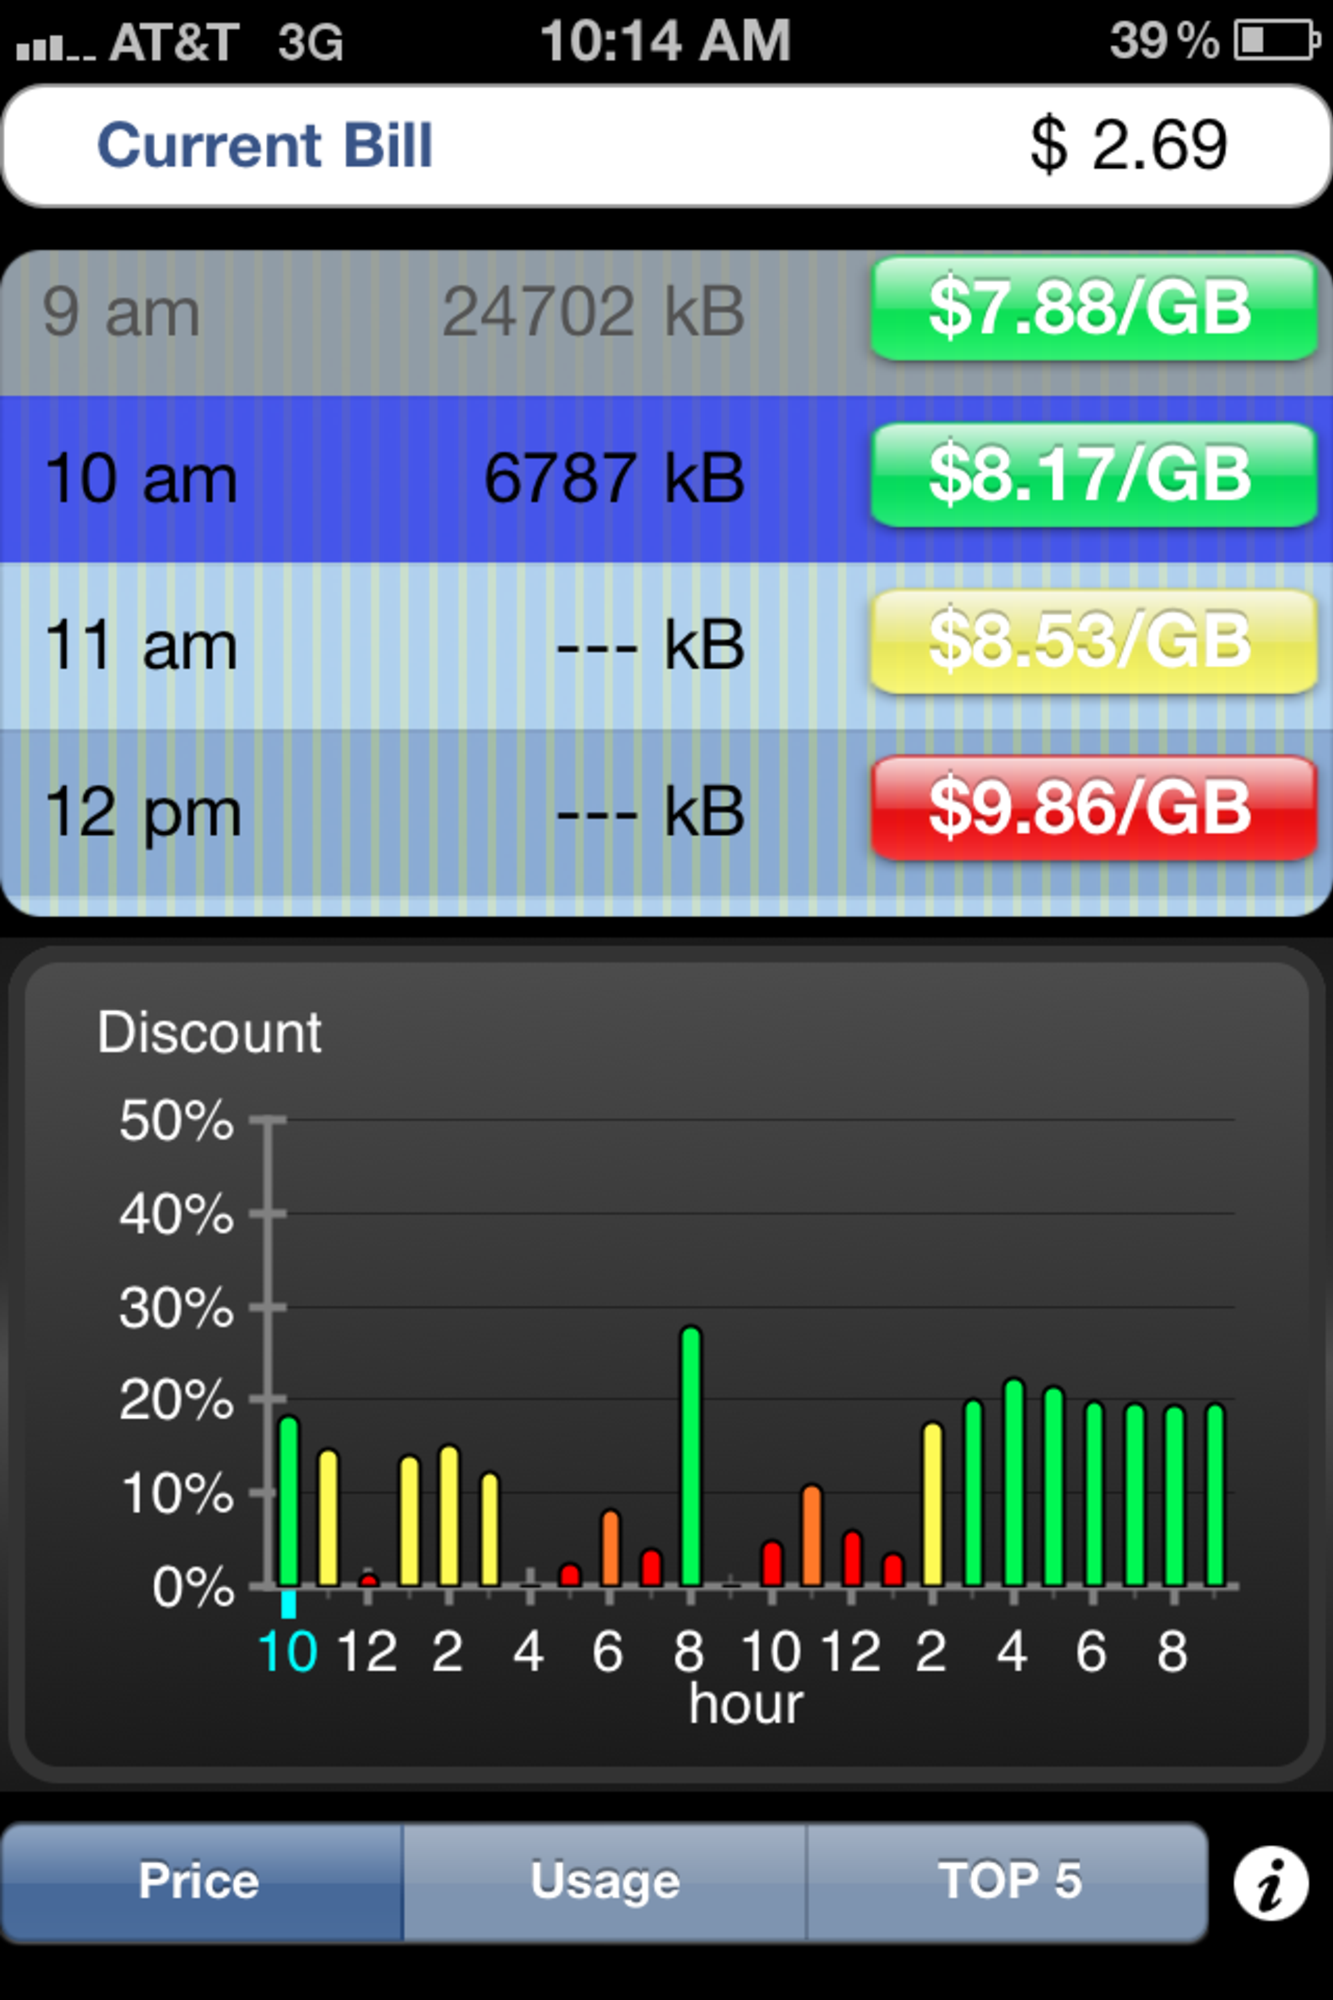
\includegraphics[width=\textwidth]{Figures/iphone_ui1.pdf}
	\caption{Price display.}
\end{subfigure}
%
\begin{subfigure}[b]{0.22\textwidth}
	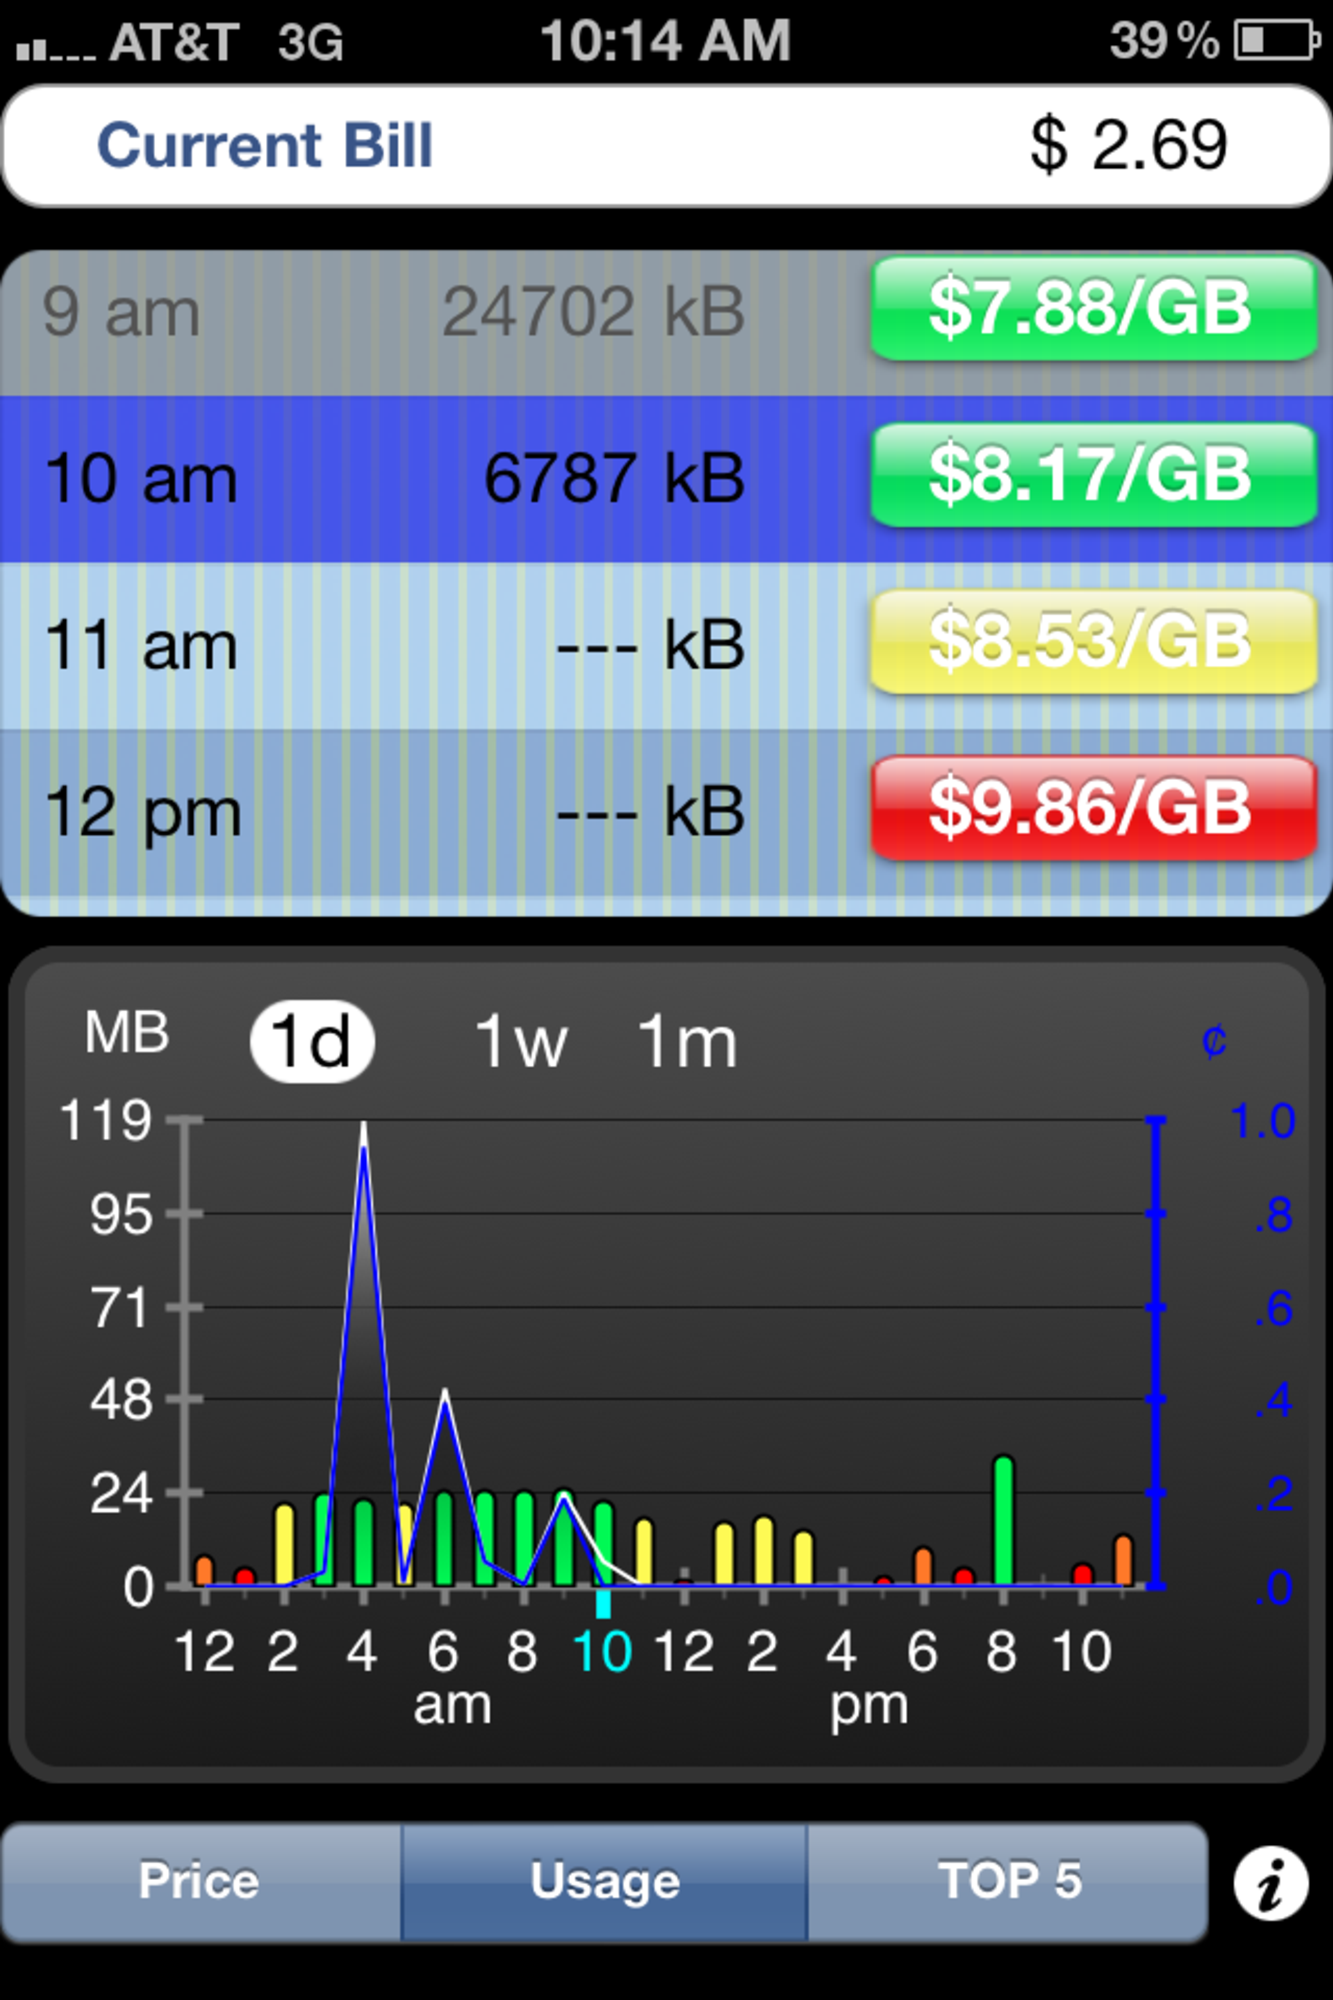
\includegraphics[width=\textwidth]{Figures/iphone_ui2.pdf}
	\caption{Price and usage.}
\end{subfigure}
%
\begin{subfigure}[b]{0.22\textwidth}
	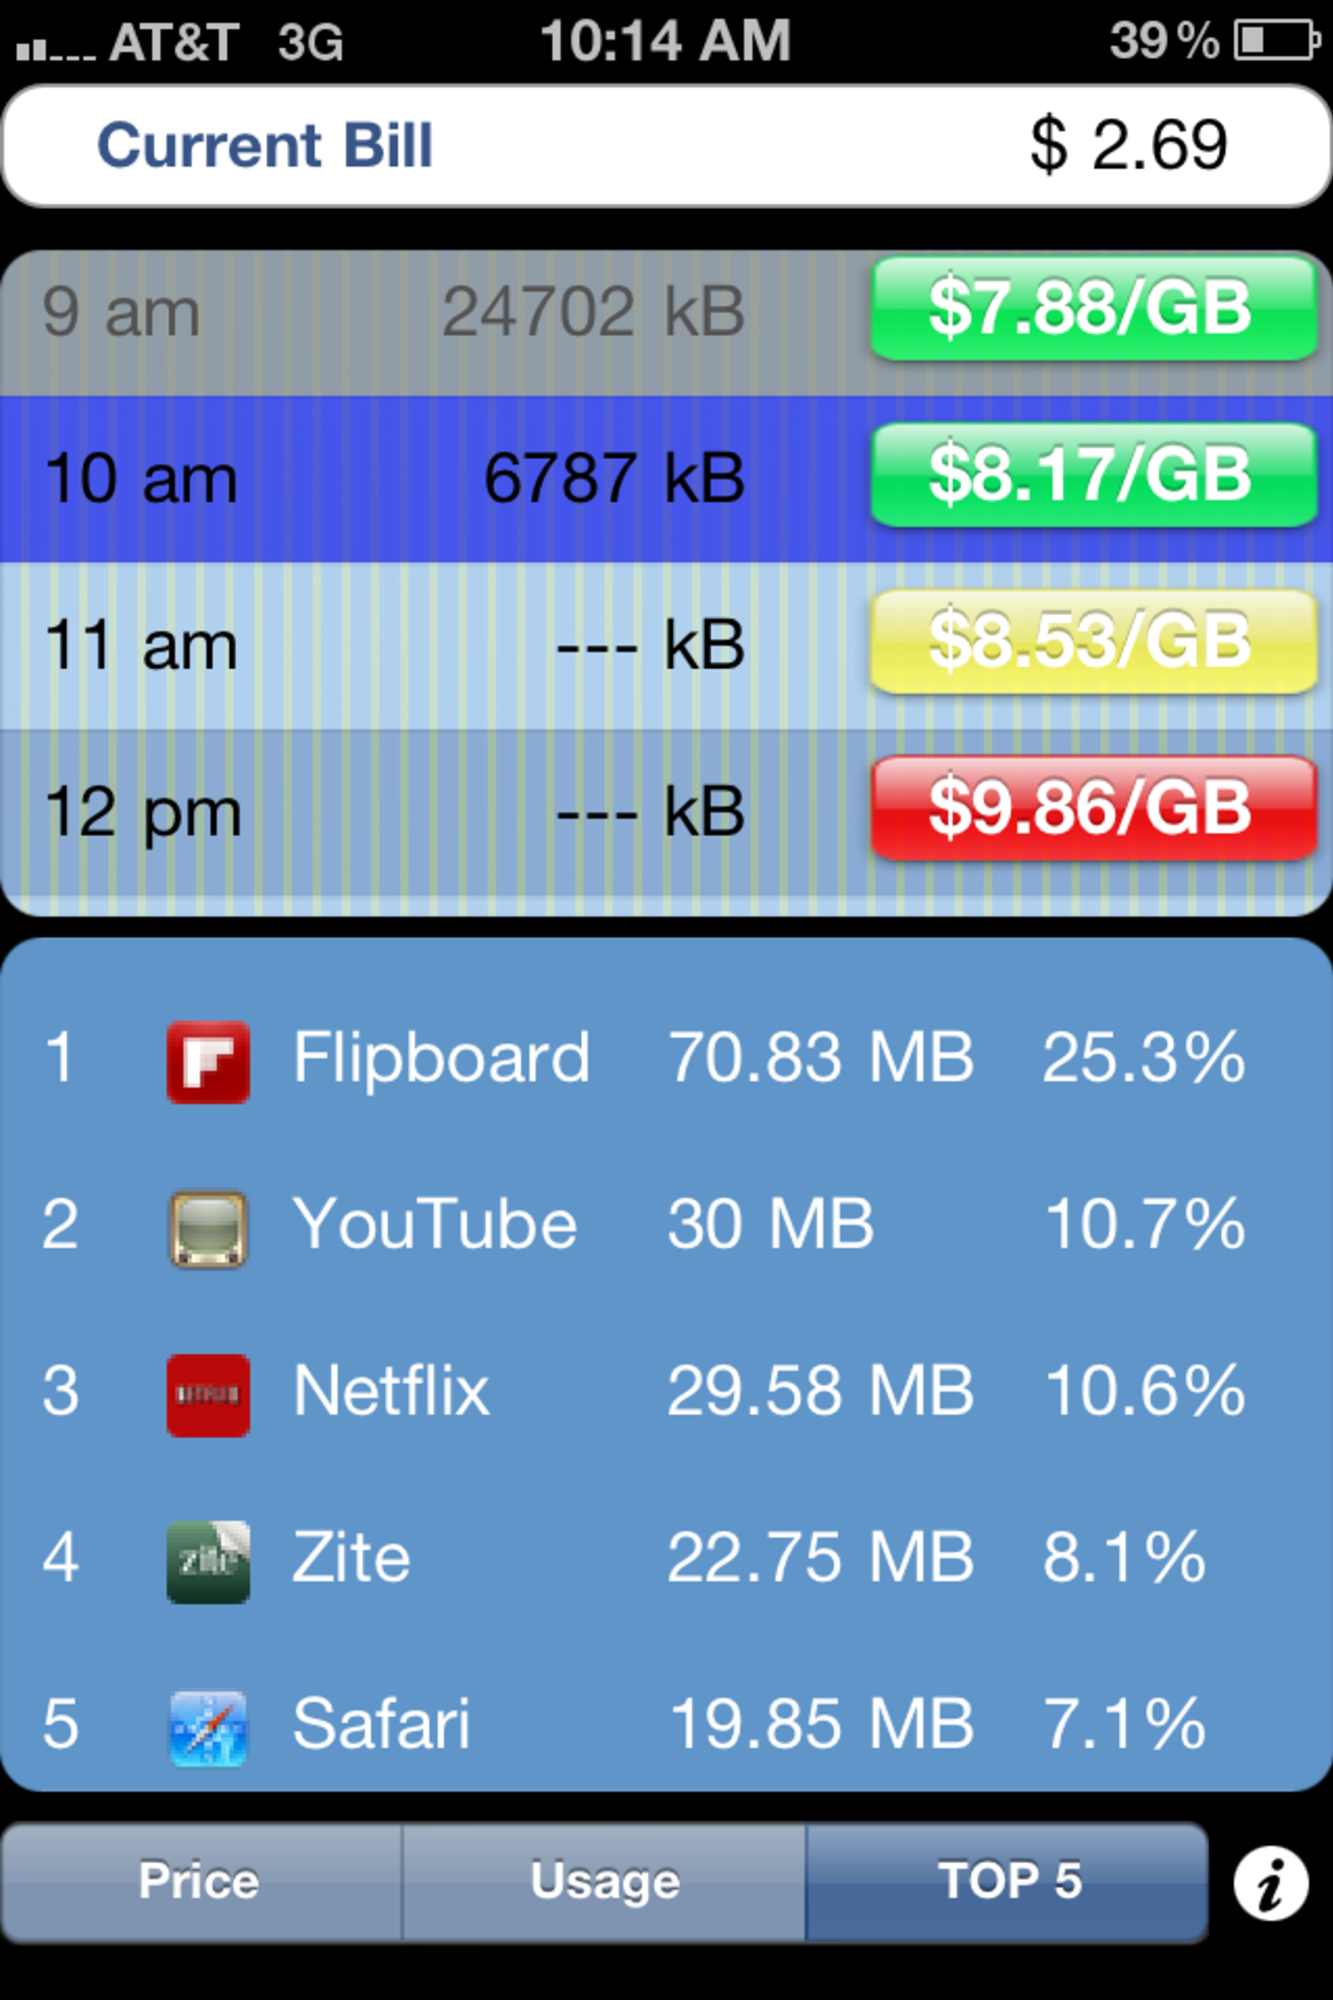
\includegraphics[width=\textwidth]{Figures/iphone_ui3.pdf}
	\caption{Top 5 applications.}
\end{subfigure}
%
\begin{subfigure}[b]{0.22\textwidth}
	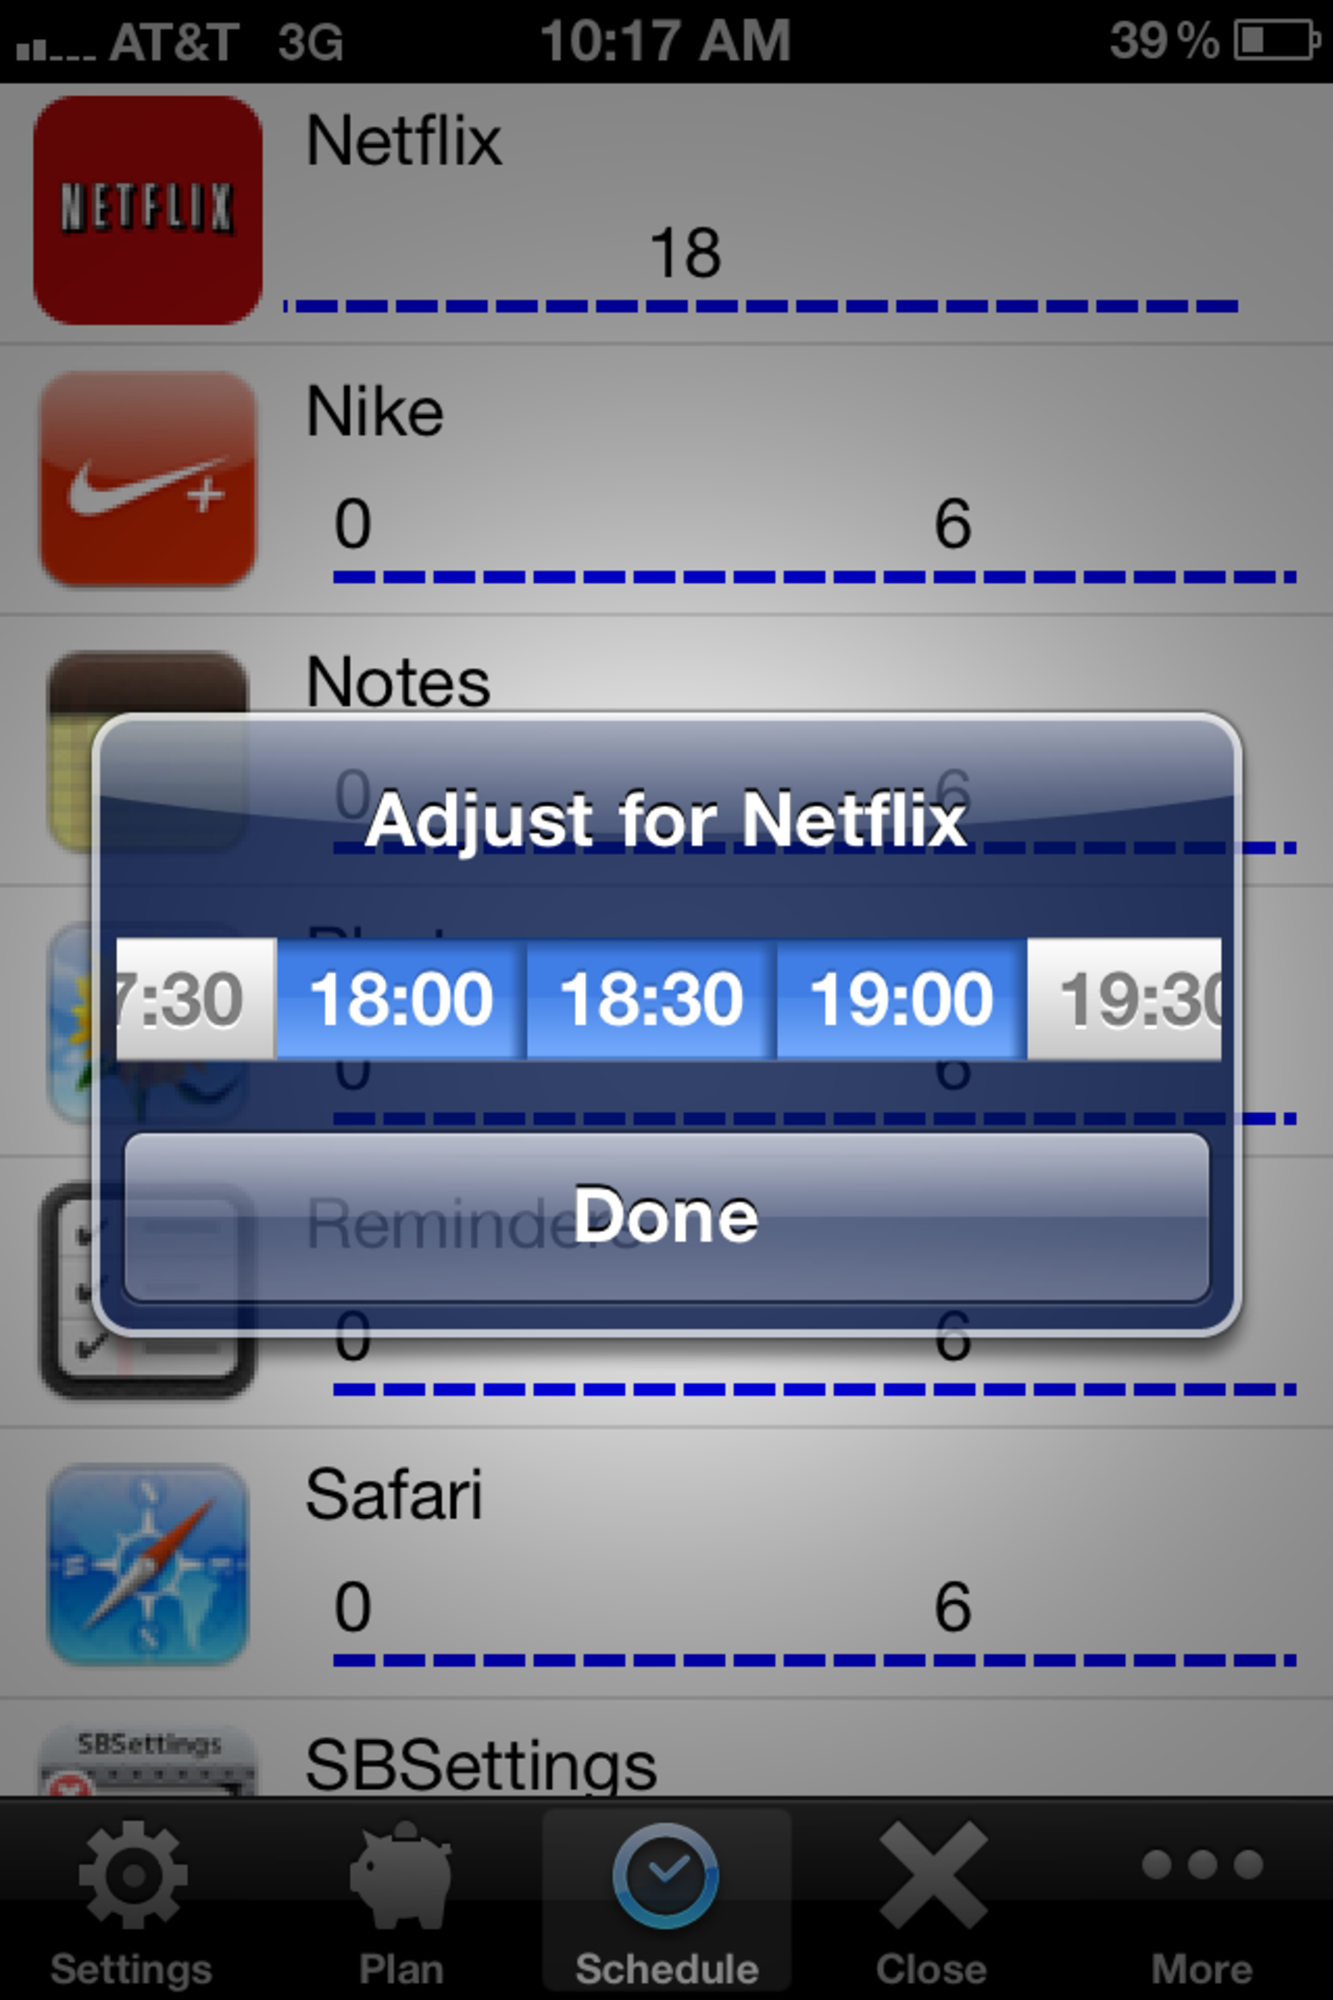
\includegraphics[width=\textwidth]{Figures/iphone_ui5.pdf}
	\caption{App scheduling.}
\end{subfigure}
\end{center}
\vspace{-0.25in}
\caption{Screenshots of user interfaces for time-dependent pricing. Users can (a) check the prices for next 24 hours, (b) view their price and usage history, (c) identify the top 5 apps by bandwidth usage, and (d) schedule their apps at different times of the day.}
\label{fig:tube_gui}
\vspace{-0.05in}
\end{figure}

\subsection{Trial Results}

Recently, the authors of the present work developed a prototype of the above pricing algorithms, system components, and user interfaces and trial-ed it with 50 end users \cite{ha2012tube}. We here present some results from this TUBE trial, which illustrate both the importance of user interface design and the effectiveness of optimized TDP. % We also interviewed trial participants after the trial was complete. Not only did participants express appreciation for TDP's ability to offer price discounts, they also agreed in general with SDP's philosophy of more intelligent pricing for data to help users save money and ISPs reduce congestion. Users' openness to these new pricing plans signals that, with the right pricing algorithms and effective system and UI designs, new forms of data pricing can be feasible in practice.

An initial phase of the TUBE trial offered alternating high (10\% discount) and low (40\% discount) time-dependent prices in different hours. After two weeks of following the high-low-low price pattern, the prices changed, repeating the pattern of a 9\% discount at midnight, followed by 28\%, 30\%, 28\%, 9\%, and 30\% discounts in subsequent hours. The home screen price indicator was green for discounts over 30\%, orange for 10--29\% discounts, and red for discounts below 10\%. % Besides being color coded, the indicator also showed the numerical discount value.

Usage in different hours with these pricing patterns can be compared to assess the effect of the indicator color and numerical discount: hours deemed as Type 1 periods offered a 10\% discount in the first stage of the experiment and 28\% discount in the second stage, with the indicator remaining orange despite this increase in the discount.  Type 2 periods offered a 10\% (orange) discount in the first stage and 30\% (green) discount in the second stage, while Type 3 periods offered a 10\% discount in the first and 9\% discount in the second stage of the experiment (the indicator was orange in both periods).  Table \ref{periodtypes} summarizes the combinations of discounts and colors used in the two stages that characterize each type of period.
\begin{table}
\renewcommand{\arraystretch}{1.1}
\centering
\caption{Period types in the color experiment.}
\vspace{-0.1in}
\begin{tabular}{|c|c|cc|cc|}
\hline
Type & Periods & \multicolumn{2}{c|}{First Stage} & \multicolumn{2}{c|}{Second Stage} \\
 & & Color & Disc. & Color & Disc. \\ \hline
1 & 2, 8, 14, 20 & Orange & 10\% & Orange & 28\% \\ \hline
2 & 3, 6, \ldots, 24 & Orange & 10\% & Green & 30\% \\ \hline
3 & 5, 11, 17, 23 & Orange & 10\% & Orange & 9\% \\ \hline
%\st{4} & \st{1, 7, 13, 19} & \st{Green} & \st{40\%} & \st{Orange} & \st{9\%} \\ \hline
%\st{5} & \st{4, 10, 16, 22} & \st{Green} & \st{40\%} & \st{Orange} & \st{28\%} \\
%\hline
\end{tabular}
\label{periodtypes}
\end{table}

To analyze the trial results, the percentage changes in usage for each type of period were computed, relative to usage without time-dependent prices. These changes showed that \emph{users responded more to changes in the price indicator color than changes in the numeric value of the TDP discounts.} In post-trial interviews, nearly all of the trial participants indicated that they relied on the price indicator colors to know the current prices, rather than opening the TUBE app.

Figure \ref{fig:OHP_OLP_OHP} compares the usage changes observed in different period types. Each data point represents one user's average change in each period type, with the size of the data point indicating the volume of usage in the second stage of the experiment.  The reference line represents equal changes in both period types considered. Figure \ref{fig:OHP_OLP_OHP}a shows the average change in usage for each user in Type 1 periods versus Type 3 periods.  For both period types, the color did not change, but the discount in Type 1 periods increased significantly.  Thus, if users had reacted to the numerical prices, usage should increase in Type 1 and decrease in Type 3 periods: users' data points should lie above the reference line.  Figure \ref{fig:OHP_OLP_OHP}a shows that this is the case with only half of the users.  Since the indicator color did not change, users were mostly agnostic to the numerical values of the discounts.
\begin{figure*}
\centering
	\begin{subfigure}[b]{0.51\textwidth}
		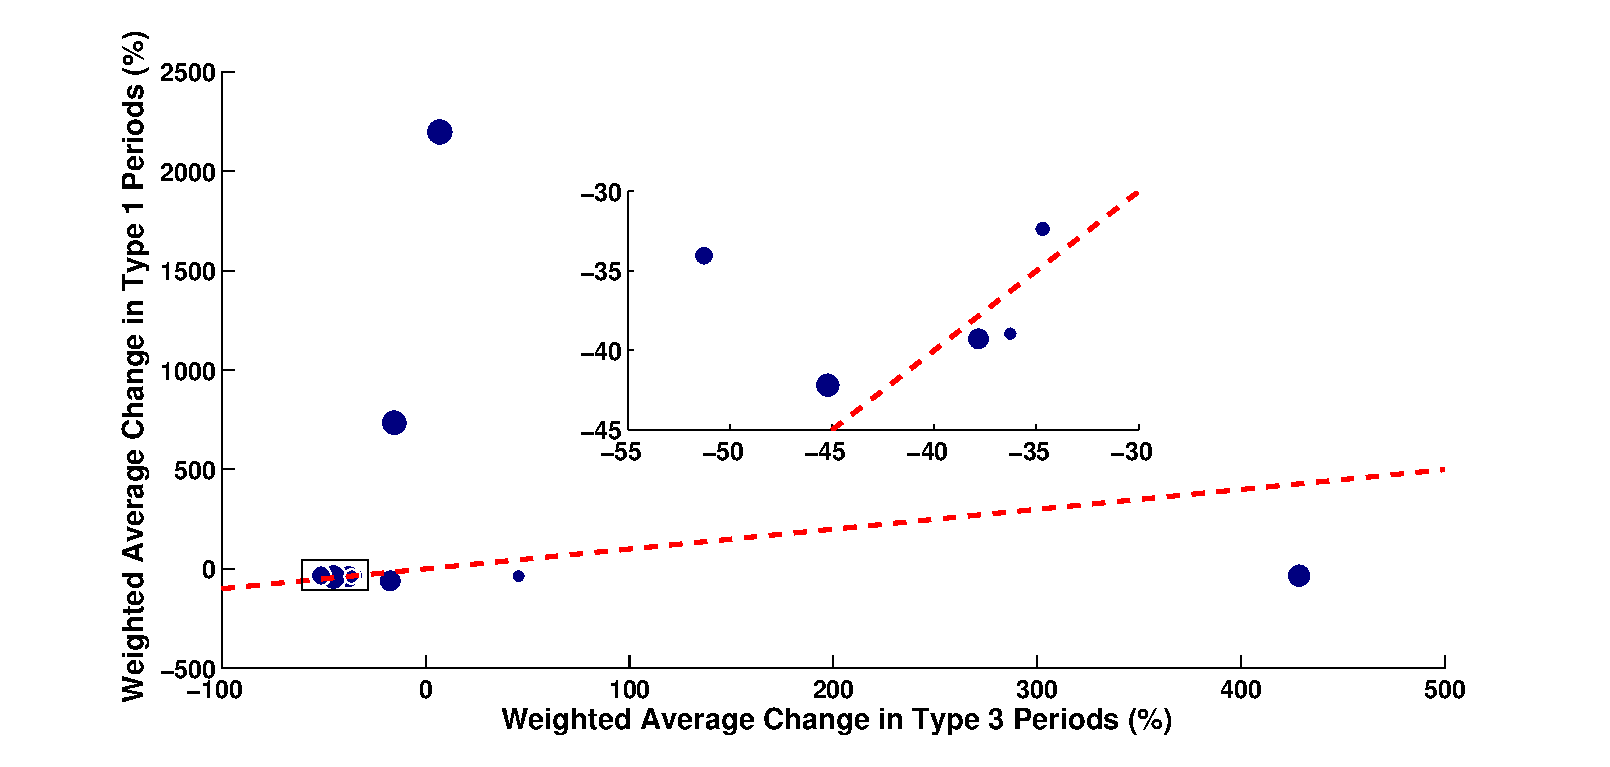
\includegraphics[width = \textwidth]{Figures/OHP_OLP_OHP.eps}
		\caption{Period types 1 and 3.}
	\end{subfigure}
	\hspace{-0.05\textwidth}
	\begin{subfigure}[b]{0.51\textwidth}
		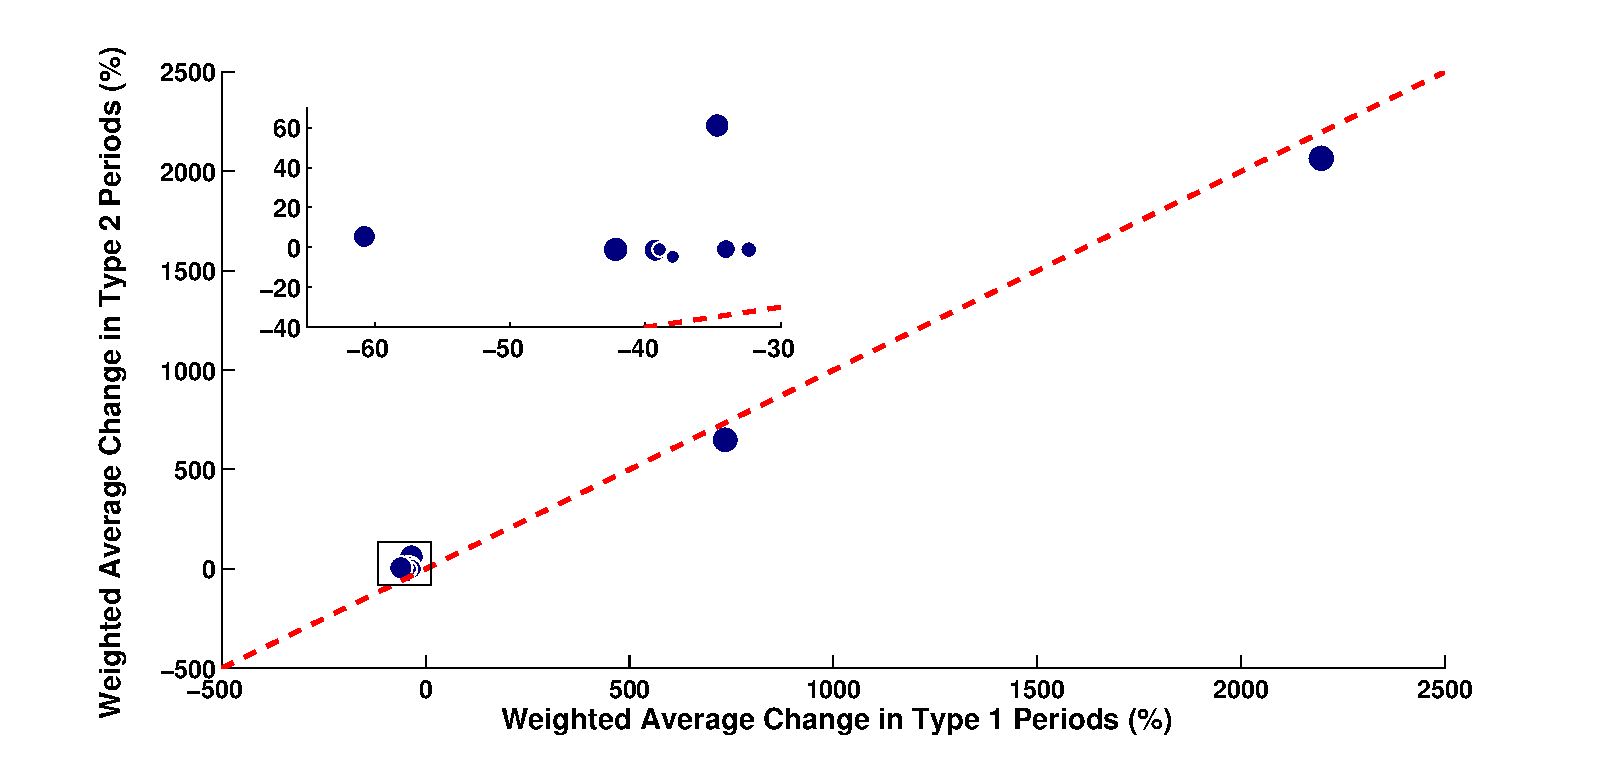
\includegraphics[width = \textwidth]{Figures/OHP_GLP_OLP.eps}
		\caption{Period types 1 and 2.}
	\end{subfigure}
\vspace{-0.1in}
\caption{Average percent changes in usage for the period types in Table \ref{periodtypes}. Users' usage behavior is (a) not affected by the prices when only the numerical discounts, but not the indicator color changes. When (b) both the color and numerical discount change, users increase their usage behavior more in low-price periods.}
\label{fig:OHP_OLP_OHP}
\vspace{-0.1in}
\end{figure*}
Figure \ref{fig:OHP_OLP_OHP}b plots the average change in usage in Type 2 versus Type 1 periods.  The discounts in both periods increased by comparable amounts, but the indicator color changed from orange to green only in Type 2 periods.  Most users' data points lie above the reference line, indicating that usage increased more (or decreased less) in Type 2 as compared to Type 1 periods. Thus, users responded to the indicator color despite the comparable numerical discounts. In fact, 80\% of our participants admitted to this behavior when asked in post-trial interviews whether they paid attention to the indicator color, numerical discounts, or both.

The final stages of the trial offered optimized time-dependent prices, with initial user behavior estimates based on the usage observed in previous stages of the trial with non-optimized prices.  The reduction in peak traffic was measured by the \emph{peak-to-average ratio} (PAR), i.e., the ratio of usage in the peak period to average per-period usage, for each day.  Comparing the PARs from before and after optimized TDP reveals that \emph{optimized time-dependent prices reduce the peak-to-average ratio} from usage before time-dependent prices were offered (time-independent pricing, or TIP).  Moreover, \emph{overall usage significantly increased} after TDP was introduced, partially because people used more in the discounted valley periods. % Valley filling and peak reduction together contributed to lower peak-to-average ratios with TDP.
% Part of this increase is likely due to different times of the year, but we conjecture that the discounts offered with TDP induced people to spend more.

Figure \ref{fig:par}a shows the distribution of daily PARs both before and after TDP was introduced.  The maximum PAR decreases by 30\% with TDP, and approximately 20\% of the PARs before TDP are larger than the maximum PAR with TDP.  Thus, TDP significantly reduced the peak-to-average ratio, flattening demand over the day. Moreover, this decrease in PAR is not due to a net loss of traffic.  Figure \ref{fig:par}b shows the average per-user daily usage observed before and after TDP.  The overall volume of usage after TDP is greater than that before TDP; in fact, across all users, the average change in usage from TIP to TDP is a 130\% increase.  Part of this increase may be due to the time of year--TIP usage was measured from July to September, and the TDP usage in January. TDP, however, is likely a major factor: the discounts during off-peak periods allowed users to consume more data while still spending less money and decreasing the PAR. In fact, in post-trial interviews 30\% of the trial participants admitted to consciously using more data in the heavily discounted periods, with one explicitly comparing the situation to shopping at a clothing sale in department stores.
\begin{figure*}
\centering
	\begin{subfigure}[b]{0.42\textwidth}
		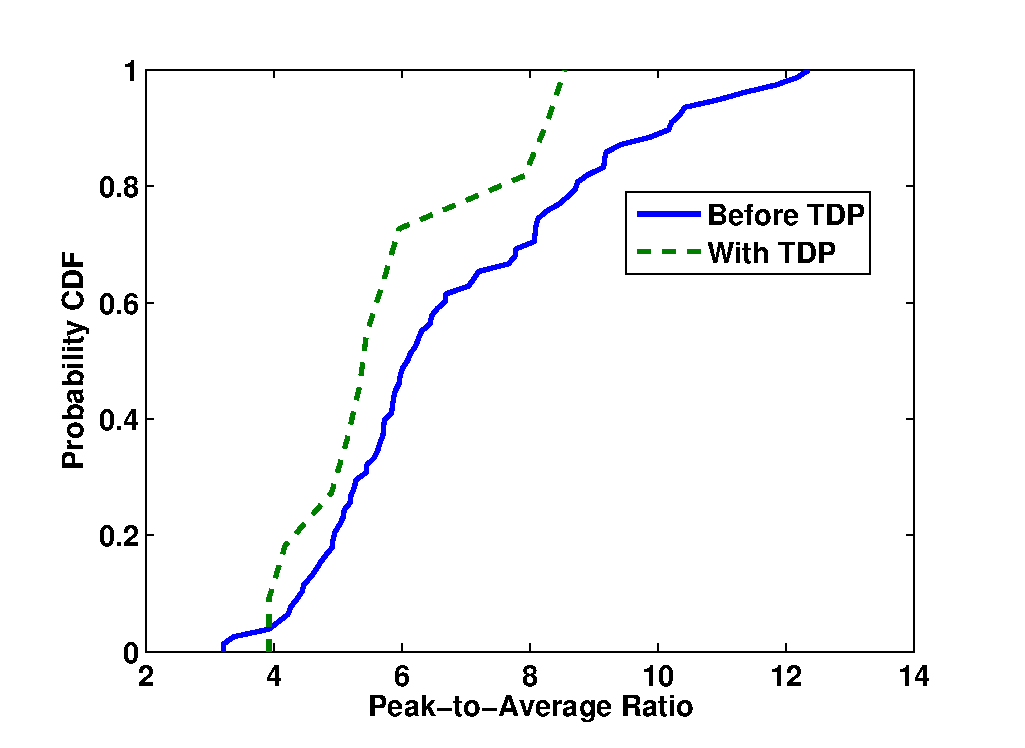
\includegraphics[width = \textwidth]{Figures/PAR.eps}
		\caption{PARs.}
	\end{subfigure}
	\hspace{-0.03\textwidth}
	\begin{subfigure}[b]{0.42\textwidth}
		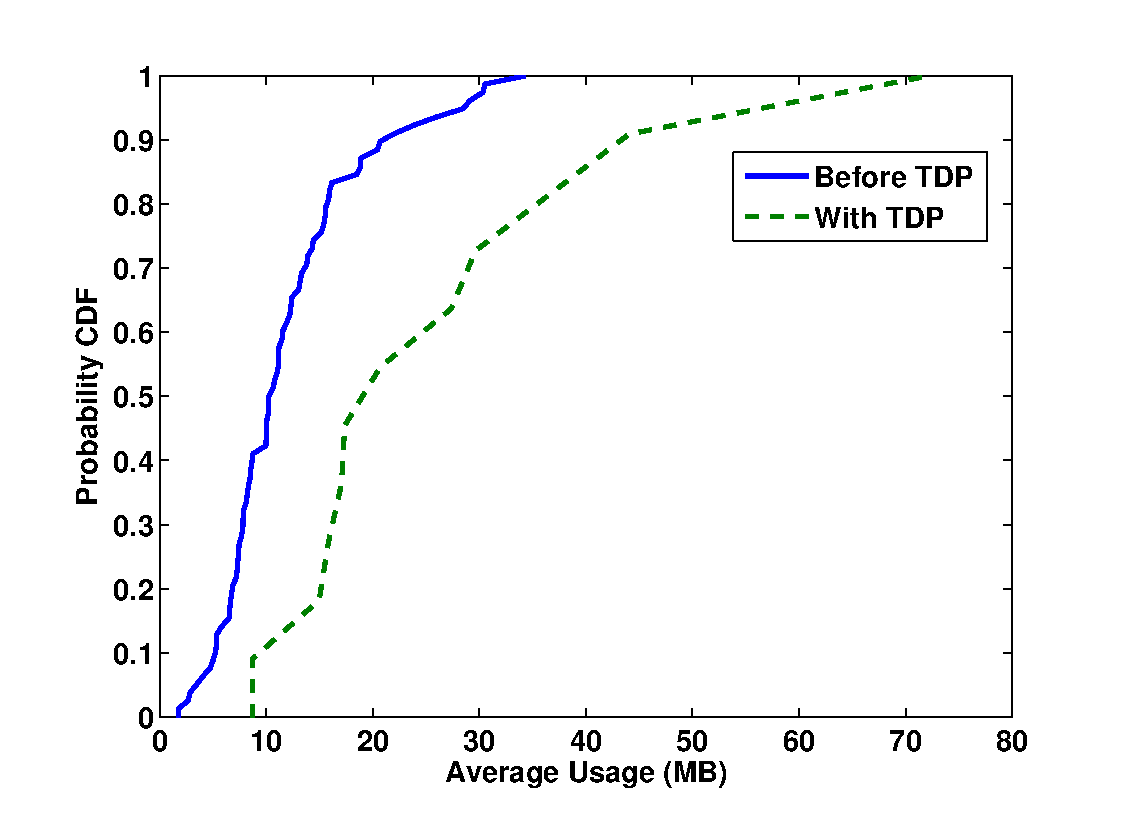
\includegraphics[width = \textwidth]{Figures/Avg.eps}
		\caption{Average daily traffic.}
	\end{subfigure}
\vspace{-0.1in}
\caption{Usage statistics in the TIP (time-independent pricing) and optimized TDP phases of the TUBE trial. When optimized TDP is offered, (a) the ISP's peak-to-average ratio generally decreases, while (b) the average daily traffic per user increases.}
\label{fig:par}
\vspace{-0.1in}
\end{figure*}

\section{20 Open Questions and Future Directions}\label{sec:20Q}

Current trends and future directions in smart pricing practices aim to make proposed pricing plans economically viable. For instance, substantial research has been done on day-ahead pricing, including the development of carefully designed user interfaces to display price and usage data as shown in Figure \ref{fig:tube_gui}. Incorporating human factors into the engineering and design phase along with economic models can provide a holistic approach in solving the challenges of network congestion.
%More generally, client-side architectures may ease the user burden of dynamic pricing plans; however, the design of such components remains an open problem, and this conjecture has not yet been thoroughly tested on real users.

In addition to the pricing plans proposed above, new pricing plans have recently been proposed that have been rarely studied in the academic literature. Some promising directions include the following:

\begin{figure}
\centering
\begin{subfigure}[b]{0.23\textwidth}
	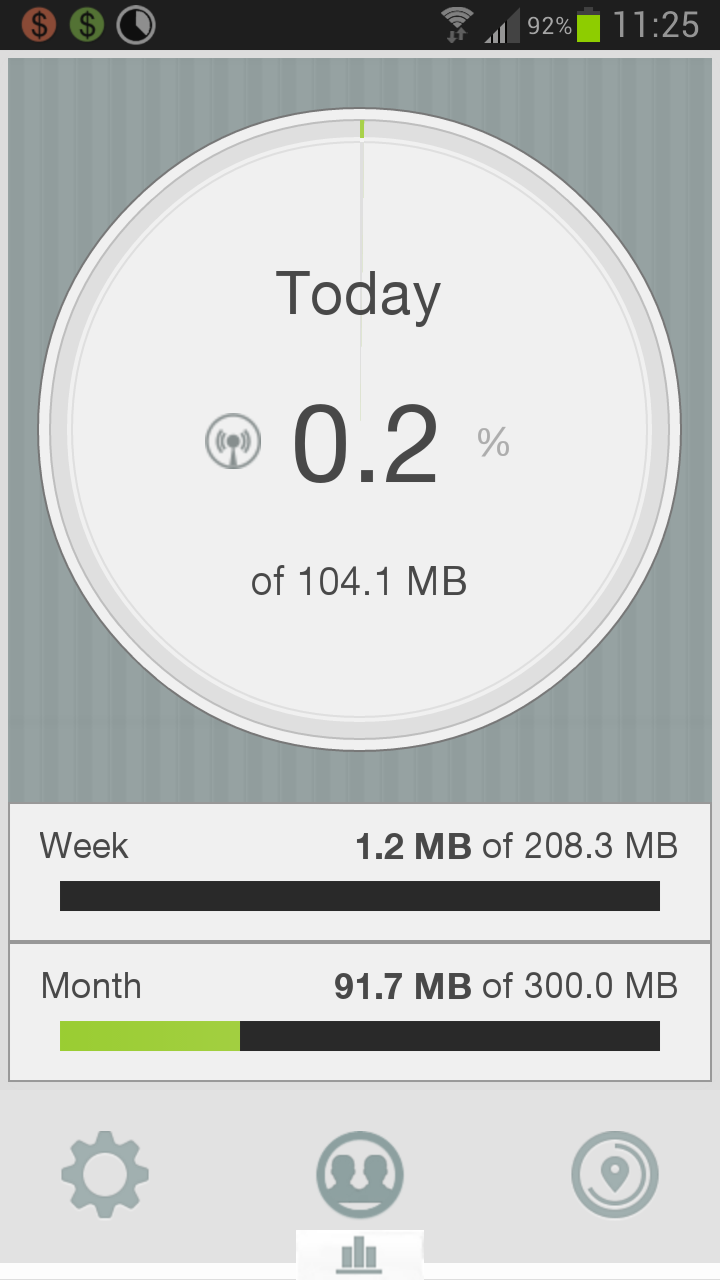
\includegraphics[width = \textwidth]{Figures/Main.png}
	\caption{Home screen.}
	%\vspace{0.05in}
	\label{fig:datawiz_main}
	\end{subfigure}
	\begin{subfigure}[b]{0.23\textwidth}
	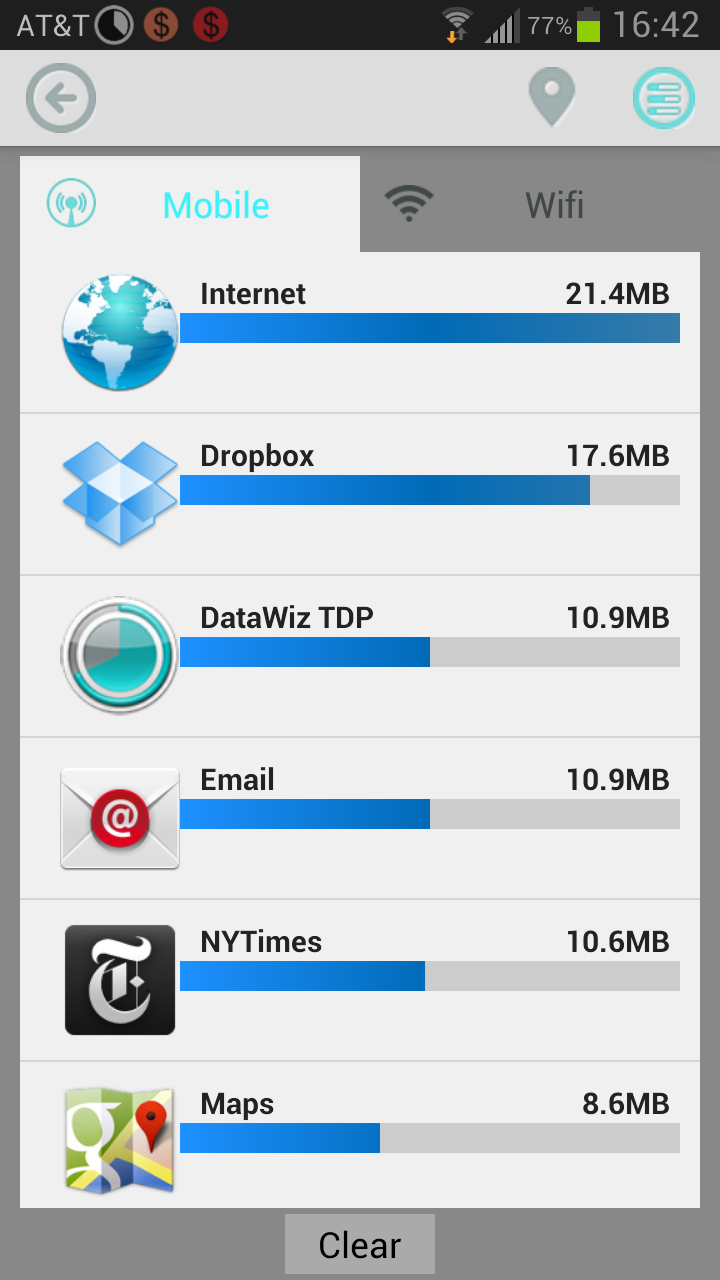
\includegraphics[width = \textwidth]{Figures/Apps_Mobile.png}
	\caption{Cellular usage per app.}
	%\vspace{0.05in}
	\label{fig:datawiz_main_graph}
	\end{subfigure}
	\begin{subfigure}[b]{0.23\textwidth}
	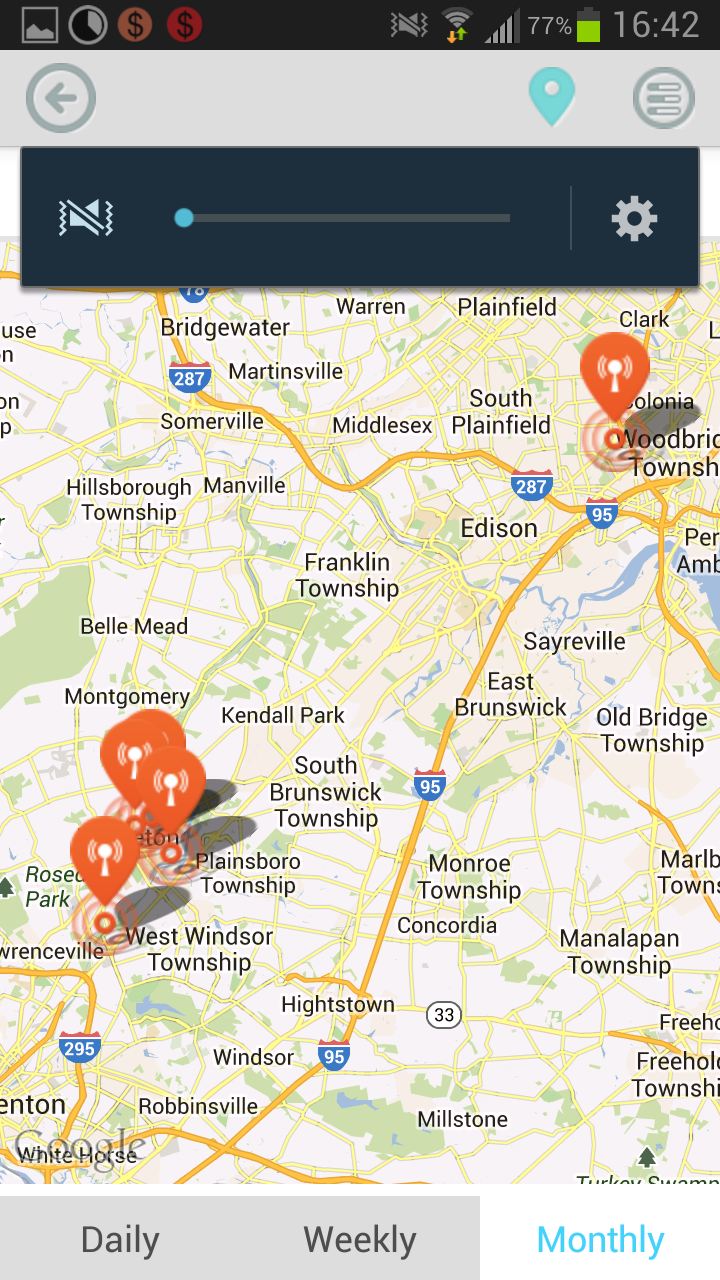
\includegraphics[width = \textwidth]{Figures/Maps.png}
	\caption{Usage locations.}
	%\vspace{0.05in}
	\label{fig:datawiz_predict}
	\end{subfigure}
	\begin{subfigure}[b]{0.23\textwidth}
	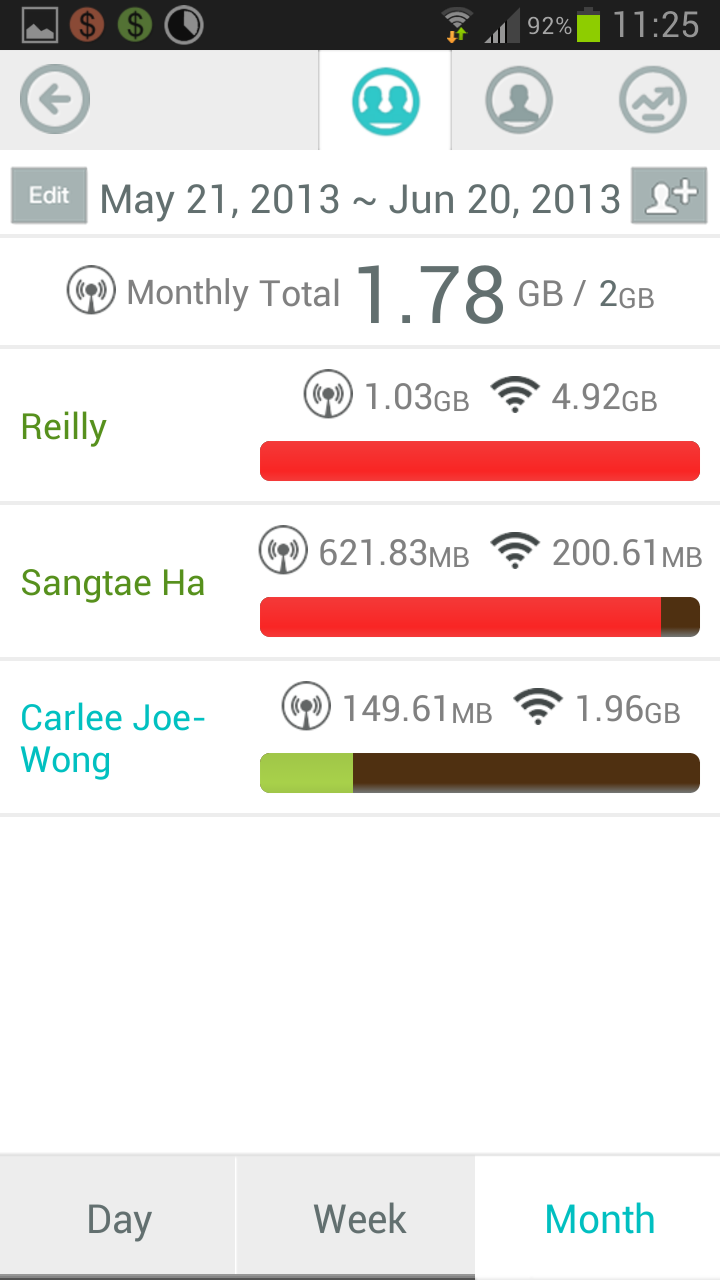
\includegraphics[width = \textwidth]{Figures/Members.png}
	\caption{Shared usage.}
	%\vspace{0.05in}
	\label{fig:datawiz_map2}
	\end{subfigure}
	
	\vspace{0.3in}
	
	\begin{subfigure}[b]{0.23\textwidth}
	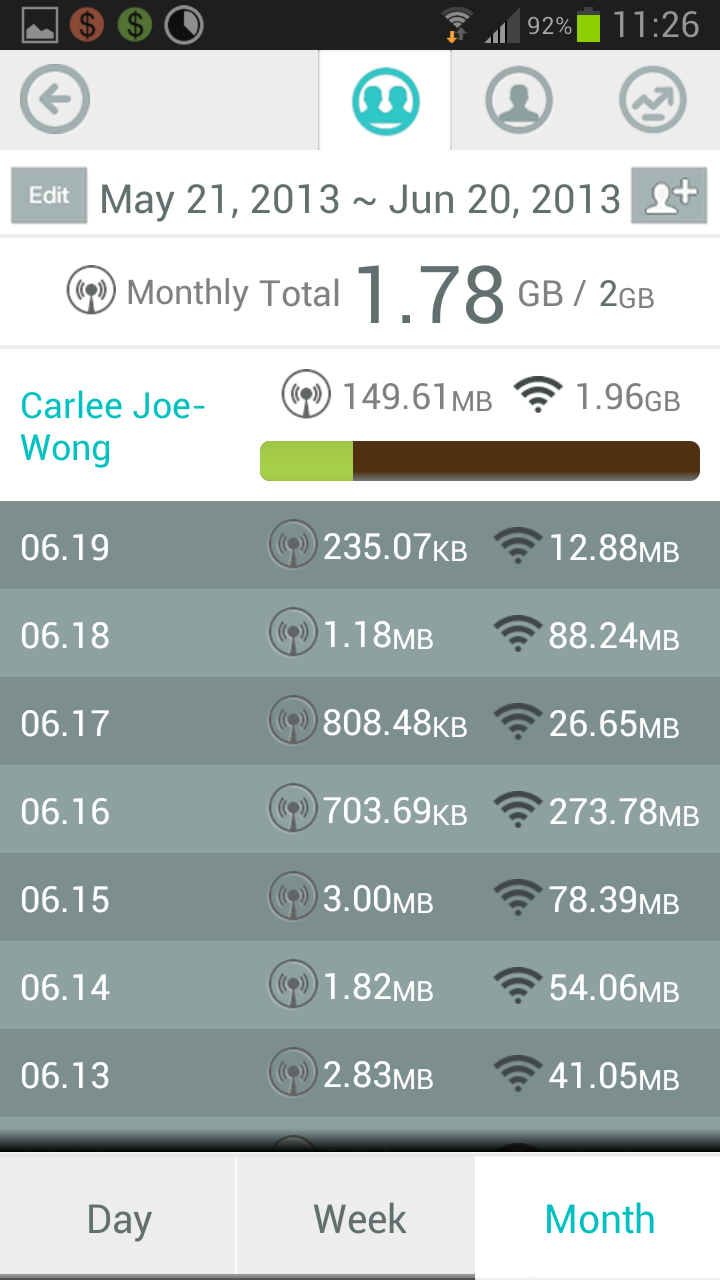
\includegraphics[width = \textwidth]{Figures/Usage.png}
	\caption{Individual usage.}
	%\vspace{-0.05in}
	\label{fig:datawiz_indv}
	\end{subfigure}
	\begin{subfigure}[b]{0.23\textwidth}
	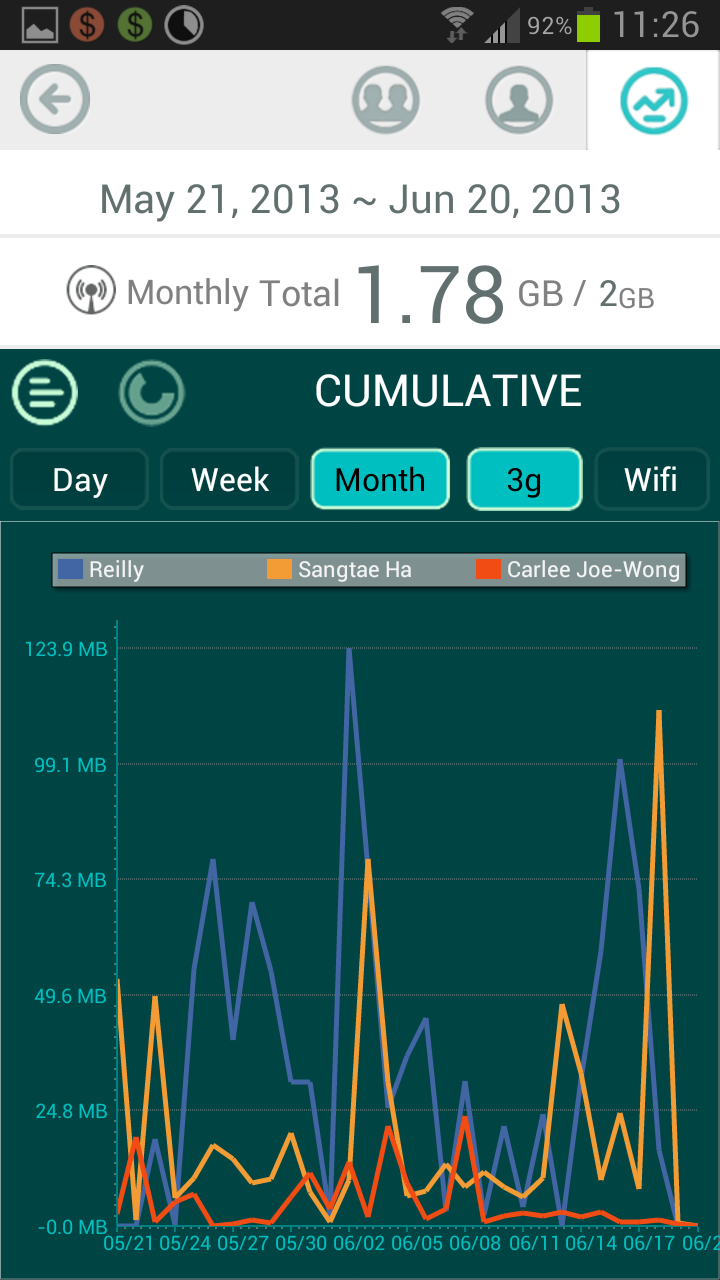
\includegraphics[width = \textwidth]{Figures/Line_Graph.png}
	\caption{Usage over time.}
	%\vspace{-0.05in}
	\label{fig:datawiz_time}
	\end{subfigure}
	\begin{subfigure}[b]{0.23\textwidth}
	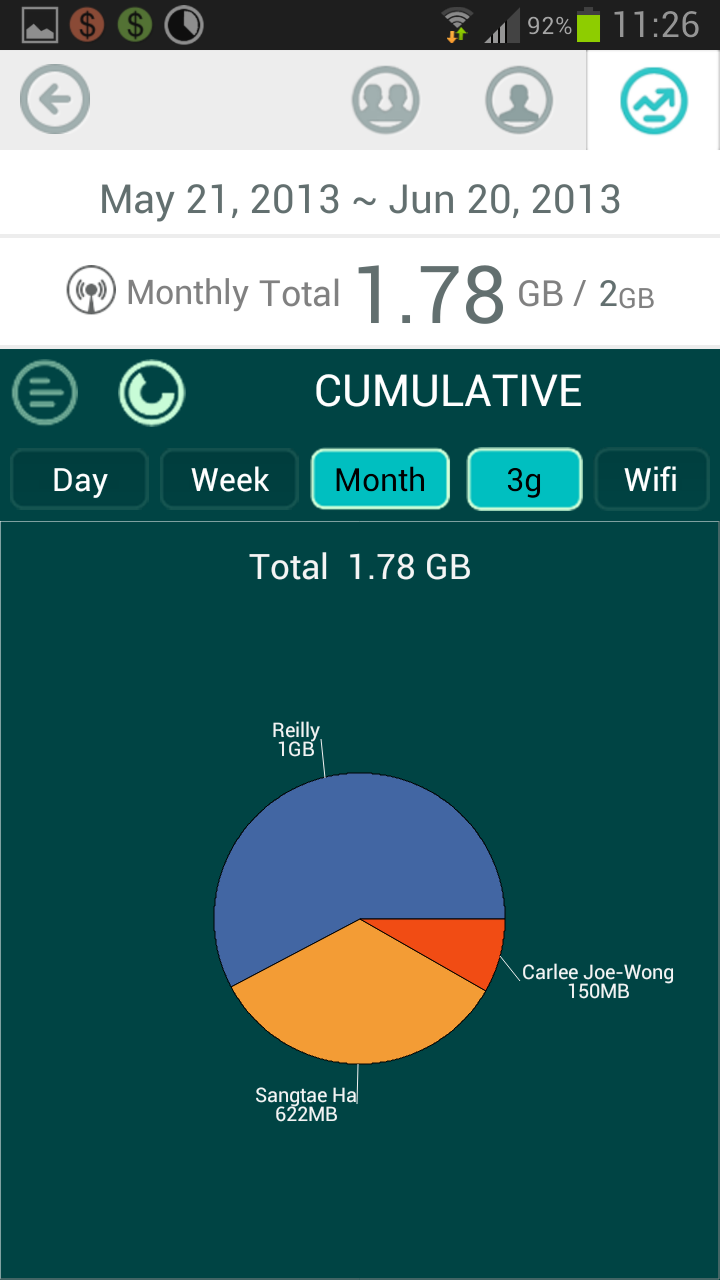
\includegraphics[width = \textwidth]{Figures/Pie_Chart.png}
	\caption{Usage distribution.}
	%\vspace{-0.05in}
	\label{fig:datawiz_pie}
	\end{subfigure}
	\begin{subfigure}[b]{0.23\textwidth}
	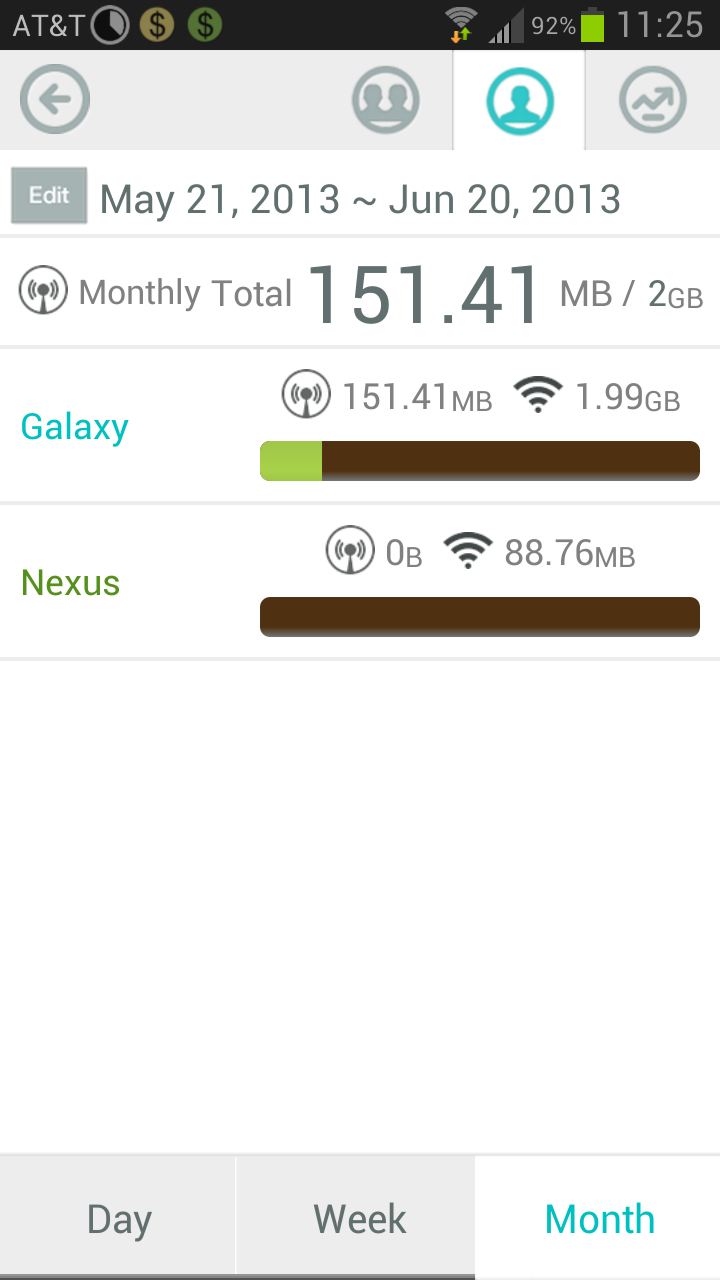
\includegraphics[width = \textwidth]{Figures/Devices.png}
	\caption{Usage of devices.}
	%\vspace{-0.05in}
	\label{fig:datawiz_device}
	\end{subfigure}
\caption{Screenshots of the DataWiz app with shared data plans. A user can add other users or devices to her shared data plan and can keep track of the shared data usage as well as individual usage. When a user is requested to be a part of the shared data plan, a push notification is sent to the user and the user can either accept or reject this invitation.}
\label{fig:datawiz}
\end{figure}

\begin{description}
\item[Shared data plans:] AT\&T and Verizon in the United States recently introduced shared data plans, in which several devices share a common data cap. While some studies of shared data plans have been made \cite{WITS}, the effects of such plans on user behavior, and how such a data cap can be shared fairly and efficiently among users, remain to be studied in detail.

One practical challenge for users on shared data plans is keeping track of their usage across multiple devices--while many apps exist to track usage on individual devices; e.g., Onavo Count, My Data Manager, and DataWiz; none track the usage of multiple devices. In fact, tracking usage on multiple devices requires not only modifications to user interface design but also integration with a common server that can send usage information of other user devices to each device on a shared plan. A login and agreement process is also necessary to ensure that users can see each others' usage only once both users have given permission.

Screenshots of a prototype shared data plan app based on the DataWiz usage monitoring application are shown in Figure \ref{fig:datawiz}. The app lets users view their monthly, weekly, and daily usage as compared to their monthly data cap (Figure \ref{fig:datawiz_main}), as well as per-app and per-location usage (Figures \ref{fig:datawiz_main_graph} and \ref{fig:datawiz_predict}). The small pie chart indicator on the top left corner of the phone allows users to quickly see their monthly usage; the chart is filled according to how much of his or her monthly cap the user has consumed.
%
In addition to these basic features, users can add and remove other users and devices to their data plan; if a user is added to someone else's data plan, the invitation recipient receives a push notification and can accept or reject the invitation. Upon acceptance, both users may view each other's usage over time (Figures \ref{fig:datawiz_indv} and \ref{fig:datawiz_time}) and on a pie chart (Figure \ref{fig:datawiz_pie}). Users may add multiple devices to their accounts; each user's total usage is then the combined usage from all of these devices (Figure \ref{fig:datawiz_device}). A push notification is sent if a user is removed from a shared data plan.

\item[Fair throttling:] Instead of merely charging users more over a certain cap, ISPs may forcibly limit usage by throttling users to a limited bandwidth rate. However, researchers have still not thoroughly examined how these bandwidth limits should be set, how they should vary over time, and what their implications are in terms of fairness across different users.

\item[Heterogeneous networks:] Many ISPs are turning to supplementary networks such as WiFi and femtocells to offload traffic from congested cellular networks. While access to such networks is often free, in the future they may wish to implement more systematic access pricing to influence the adoption of such technologies and distribution of the user population across complementary networks like WiFi and 3G \cite{wifi-3g-infocom,Im}.

\item[Sponsored content:] A major question in pricing is ``whom to charge" for delivering traffic. In a two-sided pricing model (like in the credit card business) of the Internet, the price of connectivity is shared between content providers (CPs) and end users (EUs). ISPs become the middle man (or platform) proving the connectivity between CPs and EUs. This \emph{clearing house} or data traffic exchange market would extend the existing 1-800 model of phone-call services in the USA, which charges the callee rather than the caller. The tradeoffs in the resulting economic benefit between CPs and EUs remains to be quantified. Intuitively, end-users' access prices are subsidized by third party sponsors (e.g., advertisers, content providers etc.) and the ISPs have an additional source of revenue. Perhaps more surprisingly, content providers may also stand to gain from two-sided pricing if subsidizing connectivity to end-users translates into a net revenue gain through a larger amount of consumption. However, the gain to content providers depends on the extent to which content-provider payment translates into end-users' subsidy, and on the demand elasticities of the consumers. The precise gains to the three entities will therefore depend on the respective bargaining powers stemming from their contributions and price sensitivities.

Another special case of sponsored content includes \emph{zero-rating} and \emph{1-800 reverse billing} policies for data traffic. Under zero-rating, an ISP makes certain types of application traffic available to the users for free. This kind of policy, although contentious from a net neutrality viewpoint, is a major step in app-based pricing and has been practiced in some parts of Europe (e.g., Mobistar introduced a `zero-rated' plan for Facebook, Twitter, and Netlog). Understanding the impact of such pricing plans on the network ecosystem and its neutrality are important active research directions in the area of network economics.  

% \item[Time-dependent pricing:] Day-ahead pricing for mobile data has been found to be both acceptable to users and effective at reducing the network's peak load in a small pilot trial \cite{ha2012tube}. Yet it remains to be seen whether these results hold for a larger sample of users.
\end{description}

\subsection{Static Pricing}

Usage-based static pricing has traditionally been offered by ISPs around the world, and is in some sense the simplest and least controversial form of SDP. Yet even simple caps on monthly usage require a means to communicate those caps to users and, on the ISP side, accounting infrastructure to keep track of users' remaining quotas. Pricing plans like token bucket pricing or negotiated contracts require even more interaction with end users, leading to questions that include:
\begin{enumerate}
\item
How can users use their quota efficiently and keep track of a monthly usage quota?
\item
If users choose different QoS levels or times to receive better QoS, e.g., in Paris metro or token bucket pricing, how can they do so without much technical knowledge of what ``QoS''  means? How can the ISP's infrastructure keep track of users' choices and offer the appropriate QoS?
\item
Without such technical knowledge, how can users negotiate contracts (e.g., cumulus pricing) with ISPs? How can ISPs enforce these contracts?
\item
If the ISP offered some form of personalized (e.g., app-based) pricing, how would it measure the usage of different applications for each user? Where in the network should such measurements take place (i.e., client devices or the network core)? From a regulatory perspective, does this violate privacy or network neutrality concerns?
\item
How will users share the monthly data quotas imposed by shared data plans among different devices?
\end{enumerate}
%Many ISPs and third party developers, including a team led by the authors, have already released mobile apps that tell users how much of their monthly quota is left \cite{datawiz}. Yet the effects of such applications are still unclear, and little research has been done on the \emph{design} of such apps. Similarly, there has been relatively little work on automating QoS choices or negotiations for users, and the feasibility of app-based pricing or other personalized data plans remains in question.

\subsection{Dynamic Pricing}
While static pricing offers some challenges in communicating between ISPs and end users, dynamic pricing introduces even more complications as the user must be informed of changes in price. Deployment questions unique to dynamic pricing include:
\begin{enumerate}
\setcounter{enumi}{5}
\item
How often should the prices change? Should they change with the network congestion, or should they change only after a fixed time interval (e.g., one hour)?
\item
Should users be told the prices in advance? Will they accept or respond to prices that change in real time?
\item
The answer to the previous question can be more broadly phrased as follows--how can users be appropriately informed of the changing prices (e.g., with an app on their mobile devices)? What kind of design is optimal for such an app? Going further, what mechanisms can be developed to help users adjust their behavior in response to the prices?
\item
In the context of mobile data, network bottlenecks are generally highly location-dependent. Should the prices vary by location as well as by time? How will this affect users who move from one location to another?
\item
How can the prices be computed efficiently? Should this computation be done online or offline? What usage monitoring must take place, and how real time does it need to be?
\item
In addition to efficient usage monitoring, how can the ISP anticipate user reactions to the prices so as to set the ``optimal" prices? How can these change over time? Does the measurement process adequately protect user privacy?
\item
Should dynamic pricing be coupled to QoS? If so, how?
\end{enumerate}
%A recent trial of day-ahead time-dependent pricing for mobile data addressed some of these questions by implementing hourly changes in prices, which are fixed one day in advance \cite{ha2012tube}. The prices were calculated based on aggregated usage and observed changes in aggregate usage for different pries offered, so as to make the computation scalable and protect individual users' privacy. The trial included the implementation of a client-side app that showed users their price and usage history and automatically scheduled some applications to cheaper times of the day so as to keep users' monthly expenses below a maximum budget. Yet this trial involved relatively few participants, and it did not address such questions as location-dependent bottlenecks or QoS coupling.

\subsection{Sponsored Content}

% While they look quite different in practice, both sponsored content and fair throttling naturally accommodate with content providers and government regulators, perhaps more than other forms of SDP. Thus, several unique questions arise for these particular pricing plans:
Sponsored content pricing, in which content providers and advertisers subsidize users' spending on data, has not been widely deployed, partially due to the network neutrality implications of content provider subsidies. As a relatively new type of pricing, many questions remain to be answered:
\begin{enumerate}
\setcounter{enumi}{12}
\item
What is the preferred mode of ``sponsoring'' in sponsored content/access? Should it be based on increasing the user's data cap, monetary discounts, or improved speed (e.g., less throttling)?
\item
Will content providers sponsor content on a per-transaction basis? If so, how should these transactions be metered, and how much should they charge?
\item
How can ISPs measure the cost of each transaction and develop accounting systems to keep track of content providers' sponsorship?
\item
Does the idea of ``sponsored content'' violate network neutrality? Or can it be structured in a net-neutral way, e.g., sponsoring some data usage but not specifying the application?
\end{enumerate}

\subsection{Fair Throttling and Heterogeneous Networks}

Other solutions to network congestion that do not explicitly use SDP include fair throttling and deployment of heterogeneous networks to offload traffic. Fair throttling has not been widely deployed in practice--while many ISPs do throttle users who exceed a certain usage cap, such measures are fairly crude and do not take into account users' full profiles. More sophisticated throttling, e.g., Comcast's throttling of Netflix traffic in 2007, has been controversial. In contrast, many ISPs have begun offering WiFi hotspots, but it remains unclear how effective they are in relieving congestion on mobile networks. Thus, interesting theoretical and implementation questions remain for both these types of pricing, including the following:
\begin{enumerate}
\setcounter{enumi}{16}
\item
What criteria should the ISP consider when performing ``fair'' throttling? Does measuring these criteria violate user privacy or network neutrality (e.g., throttling based on the usage of specific application types)?
\item
Should users be directly involved in prioritizing different types of traffic? How can their preferences be incorporated into the throttling algorithm without the act of declaring such preferences becoming onerous to the user?
\item
How much traffic can be offloaded to other heterogeneous networks (e.g., 4G traffic to WiFi)? How cost effective is deploying such networks as a solution to network congestion? How can ISPs estimate the monetary and spectral benefits achieved through such traffic offloading or demand shifting?
\item
If ISPs were to charge for bundled access to supplementary networks like WiFi hotspots, how would such pricing plans affect users' adoption and the overall network congestion?
\end{enumerate}

These 20 questions are only some of the key questions that arise in deploying SDP and can help researchers identify interesting topics for exploration. In the coming years, as the Internet evolves further, answering these questions and others that emerge will help determine how we access (and pay for) the Internet in a highly connected, data-driven world. 


%In response, many computer networking researchers have begun to focus on the pricing of broadband data, proposing and evaluating alternative pricing policies that aim to relieve network congestion due to increased demand.

%This unprecedented growth has been outpacing ISPs' (Internet service providers) ability to expand their network capacity, prompting ISPs to turn to new pricing plans in an effort to manage their demand for data \cite{comm-mag}. Such policies include charging based on usage volume, throttling users' bandwidth, and imposing caps on monthly usage. In response, many computer networking researchers have begun to focus on the pricing of broadband data, proposing and evaluating alternative pricing policies that aim to relieve network congestion due to increased demand.

%In the past few years, ISPs around the world have offered mainly usage-based pricing plans, which often include some form of bandwidth caps and either usage-based overage charges or throttling once users exceed their data cap \cite{computing-survey}. Figure \ref{fig:timeline} gives an overview of these different usage-based pricing plans offered by major U.S. ISPs since 2008. 

%Yet usage-based pricing often end up hurting ISPs, as they do not take into account the actual costs of network congestion at any given time \cite{Odlyzko-Public}. Some ISPs in Europe and Asia have thus begun offering smarter, more innovative plans, such as app-based or location-dependent pricing. Coupled with recent advances in pricing research, these measures indicate that pricing plans will soon change. In this book chapter, we plan to give an overview of current pricing practices and a review of relevant literature on smart data pricing (SDP).

%Motivated by rapid changes in the pricing plans offered by Internet service providers (ISPs) around the world, we propose a chapter on the pricing for mobile data. In particular, we discuss several different pricing plans that have been proposed in research works, viewing them in the context of currently offered pricing plans and various challenges unique to the pricing of broadband data.

%\section{Smart Data Pricing}

%\subsection{Mobile Data Demand: The Importance of SDP}

% \subsection{Growth in Demand for Data}

%By now, it has been well-established that the demand for mobile data is growing at unsustainable rates, and will likely continue to do so for the next several years. The often-cited Cisco Visual Networking Index predicts that mobile data will grow to a volume of 10.8 exabytes per month in 2016, while wired network traffic will increase at a compound annual growth rate of 28\% per year \cite{CiscoVNI}. This unprecedented growth has been outpacing ISPs' (Internet service providers) ability to expand their network capacity, prompting ISPs to turn to new pricing plans in an effort to manage their demand for data \cite{comm-mag}. Such policies include charging based on usage volume, throttling users' bandwidth, and imposing caps on monthly usage. In response, many computer networking researchers have begun to focus on the pricing of broadband data, proposing and evaluating alternative pricing policies that aim to relieve network congestion due to increased demand.
%
%In the past few years, ISPs around the world have offered mainly usage-based pricing plans, which often include some form of bandwidth caps and either usage-based overage charges or throttling once users exceed their data cap \cite{computing-survey}. Figure \ref{fig:timeline} gives an overview of these different usage-based pricing plans offered by major U.S. ISPs since 2008. Yet usage-based pricing often end up hurting ISPs, as they do not take into account the actual costs of network congestion at any given time \cite{Odlyzko-Public}. Some ISPs in Europe and Asia have thus begun offering smarter, more innovative plans, such as app-based or location-dependent pricing. Coupled with recent advances in pricing research, these measures indicate that pricing plans will soon change. In this book chapter, we plan to give an overview of current pricing practices and a review of relevant literature on smart data pricing (SDP).
%\begin{figure}
%\centering
%\includegraphics[width = 0.8\textwidth]{Timeline.pdf}
%\vspace{-0.1in}
%\caption{Broadband pricing plans offered by major U.S. ISPs, 2008 - 2012.}
%\label{fig:timeline}
%\vspace{-0.05in}
%\end{figure}

%\subsection{Static Pricing}\label{sec:static}
%
%Recently, AT\&T and Verizon, the two largest U.S. ISPs, switched their mobile data plans from usage-based plans with monthly caps to shared data plans, in which monthly data caps are shared between multiple devices \cite{nyt-shared}. Researchers are still trying to understand the implications of this move, e.g., its effects on cooperation between users who share the same data cap. Yet monthly data caps do not significantly help in reducing the \emph{peak} load on a network--even if their overall usage is limited, users tend to crowd onto the network at the same times of the day, resulting in significant congestion at those times. Thus, though they are relatively simple for users to understand and easy to implement, data caps and other forms of usage-based pricing (i.e., charging solely by the total usage volume) do not fully mitigate problems of network congestion.
%
%One way to help deal with these congestion issues is to vary prices by the time of the day (ToD pricing). In this pricing plan, users are charged higher usage-based rates during pre-determined peak hours of the day (e.g., during the evening or day). By charging higher prices during these more congested times, ISPs can induce users to shift some usage to lower-price times, when usage is generally lower. Yet because the peak periods are fixed and users must wait several hours for a reduced price, such pricing plans often end up creating two peaks--one during the designated ``peak'' periods, and another during designated ``off-peak'' periods, made up of delay-tolerant traffic such as software updates \cite{computing-survey}. Thus, while ToD pricing is again simple enough to be appealing to users, it fails to fully address the problem of network congestion.
%
%Many more static pricing plans have been proposed in the past, and generally involve either pre-negotiated pricing contracts with users (e.g., Parris' reservation-based pricing and Clark's expected capacity pricing) or mechanisms to offer different traffic classes with different qualities of service and prices charged (e.g., Odlyzko's Paris metro pricing). While such policies can help ISPs reduce congestion on their network and do not raise network neutrality concerns, they do require some automated mechanism for users to perform these negotiations or choose QoS classes. An overview of these and other static pricing plans can be found in \cite{computing-survey}; we plan to address these in more detail in the full book chapter.
%
%% One variation on simple flat-rate or usage-based pricing would offer multiple classes of service, requiring users to pay more for improved quality of service (QoS). A particularly elegant proposal for multiple QoS is called Paris metro pricing, taking its name from actual pricing practices on the Paris metro in the 1980s. The idea of Paris metro pricing is that users will self-select into the different service classes depending on their price--the more expensive class will have fewer users, and will thus offer superior QoS without the ISP needing to improve its infrastructure for that service class \cite{Odlyzko}.
%
%% Another form of static pricing would allow content providers to share the cost of transmitting data for the content they provide. Such two-sided pricing plans have been attacked as violating network neutrality, as bigger and wealthier content providers could offer greater subsidies on their content, thus creating dis-incentives for users to consume more expensive content from smaller providers. Yet other 
%
%\subsection{Dynamic Pricing}\label{sec:dynamic}
%
%Dynamic pricing allows ISPs more flexibility than static pricing to adjust their prices based on the network load. Thus, it allows ISPs to quickly offer higher prices if congestion is observed on the network, providing a rapid feedback signal to users that induces them to reduce their usage. Yet despite its potential gains for network efficiency, dynamic pricing faces several hurdles in terms of user adoption--most users prefer simple, easy-to-understand data plans, and they may not accept rapid, uncertain fluctuations in price \cite{Odlyzko-Public,computing-survey}.
%
%Some forms of dynamic pricing have been proposed as early as the 1990s, including auction-based plans (e.g., MacKie-Mason et al.'s Smart Market) and real-time congestion-dependent pricing (e.g., Kelly's proportional-fair pricing). While these pricing plans have been shown to improve network efficiency, they require automated ways for users to respond to real-time changes in the prices, as well as careful interface design to help users understand how they are being charged.
%
%More recently, day-ahead pricing, in which prices are guaranteed for one day in the future but change each day, has been proposed as a viable pricing plan for mobile data. In day-ahead pricing, the ISP observes user reactions to the prices offered, as measured by their usage over the day, and incorporates these observations into updated estimates of how users will react to future prices. A pilot trial of this pricing plan showed that it can effectively reduce the peak load on the network and that users do respond to prices that vary each hour \cite{ha2012tube}. For this trial, interfaces were developed for users' mobile devices that allowed them to view future prices and even automatically schedule some delay-tolerant apps to cheaper times of the day; these were crucial to the success of the pilot trial.
%
%\subsection{Future Directions in Related Areas}
%
%One important future direction for SDP is the introduction of new pricing architectures. For instance, the introduction of client-side interfaces and control modules may help make dynamic pricing viable for deployment, but will require both careful interface design and research on how best to construct this client-side architecture. While some researchers in the human-computer interaction community have conducted some experiments along these lines, much work remains to be done \cite{computing-survey}.
%
%One can also consider SDP in different contexts--for instance, heterogeneous networks, in which users can offload their traffic, e.g. from cellular to WiFI networks. Many SDP pricing plans can also be applied to electricity networks--ToD pricing, for instance, has long been practiced by electricity operators. Many networking researchers, in fact, have begun to study electricity networks and ``smart grids'' as well as more traditional broadband networks \cite{computing-survey}.

\section{Exercises}

\begin{enumerate}
\item \emph{Nash Bargaining}

Consider a single access link and suppose that its bandwidth capacity $C$ is shared by $n$ users. Let $x_i$ denote the amount of bandwidth received by each user $i = 1,2,\ldots,n$, and suppose for simplicity that each user receives utility $x_i$ from $x_i$ amount of bandwidth. Suppose that the ISP allocates bandwidth to users so as to maximize
\begin{equation}
\prod_{i = 1}^n x_i\quad{\rm s.t.}\;\sum_{i = 1}^n x_i \leq C.
\end{equation}
Show that the resulting allocation $\left\{x_i^\ast\right\}$ satisfies the four Nash bargaining axioms presented in Section \ref{sec:gametheory}.

\item \emph{Time-of-Day Smart Grid Pricing}

Taken from M. Chiang, \emph{Networked Life: 20 Questions and Answers}, Cambridge University Press, 2012.
\\ \\
Smart grid electricity providers often set time-dependent prices for energy usage.  This problem considers a simplified example with two periods, the day-time and the night-time.  The provider can set different prices for the two periods, and wishes to shift some night usage to the day.  The energy provider always offers the full price during the night, and offers a reward of \$$p$/kWh during the day.

Suppose that with uniform (not time-dependent) prices, customers vacuum at night, using 0.2 kWh, and also watch TV, using 0.5 kWh, and do laundry, using 2 kWh.  During the day, customers use 1 kWh.  The probability of users shifting vacuum usage from the night to the day is
\begin{equation}
1 - \exp\left(-\frac{p}{p_V}\right),
\end{equation}
where $p_V = 2$, and the probability of shifting laundry to the daytime is
\begin{equation}
1 - \exp\left(-\frac{p}{p_L}\right),
\end{equation}
where $p_L = 3$.  Users never shift their TV watching from the night to the day.

Suppose that the provider has a capacity of 2 kWh during the night and 1.5 kWh during the day.  The marginal cost of exceeding this capacity is \$1/kWh.  Assume that energy costs nothing to produce until the capacity is exceeded.

\begin{enumerate}
\item
Compute the expected amount of vacuum and laundry energy usage (in kWh) that is shifted from the night to the day, as a function of $p$.
\item
Find (to the nearest cent) the reward $p$ which maximizes the energy provider's profit.
\item
Suppose that if vacuum or laundry usage is shifted from the night to the day, it is shifted by 12 hours.  Compute the expected time shifted of vacuum and laundry using $p = p^\ast$, the optimal reward found above.
\end{enumerate}

\item \emph{Paris Metro Pricing}

Taken from M. Chiang, \emph{Networked Life: 20 Questions and Answers}, Cambridge University Press, 2012.
\\ \\
Consider a metro system where two kinds of services are provided: service class $1$ and service class $2$. Let $p_1$, $p_2$ be the one-off fees charged per user when accessing service classes 1 and 2 respectively. Suppose each user is characterized by a valuation parameter $\theta\in [0,1]$ such that its utility of using service class $i$ is
$$U_{\theta}(i)=(V-\theta K(Q_i,C_i))-p_{i},$$
where $V$ is the maximum utility of accessing the service, $K(Q_i,C_i)$ measures the amount of congestion of service class $i$, given $Q_i\geq 0$ as the proportion of users accessing service class $i$ (with $\sum_i Q_i=1$), and $C_i\geq0$ is the proportion of capacity allocated to service class $i$ (with $\sum_i C_i=1$).

At the equilibrium, i.e., no user switches from his selection, $U_{\theta}(i)$ is merely a linear function of $\theta$. Suppose the equilibrium is illustrated as in Figure \ref{fig:equilibrium}.\\

\begin{figure}
\centering
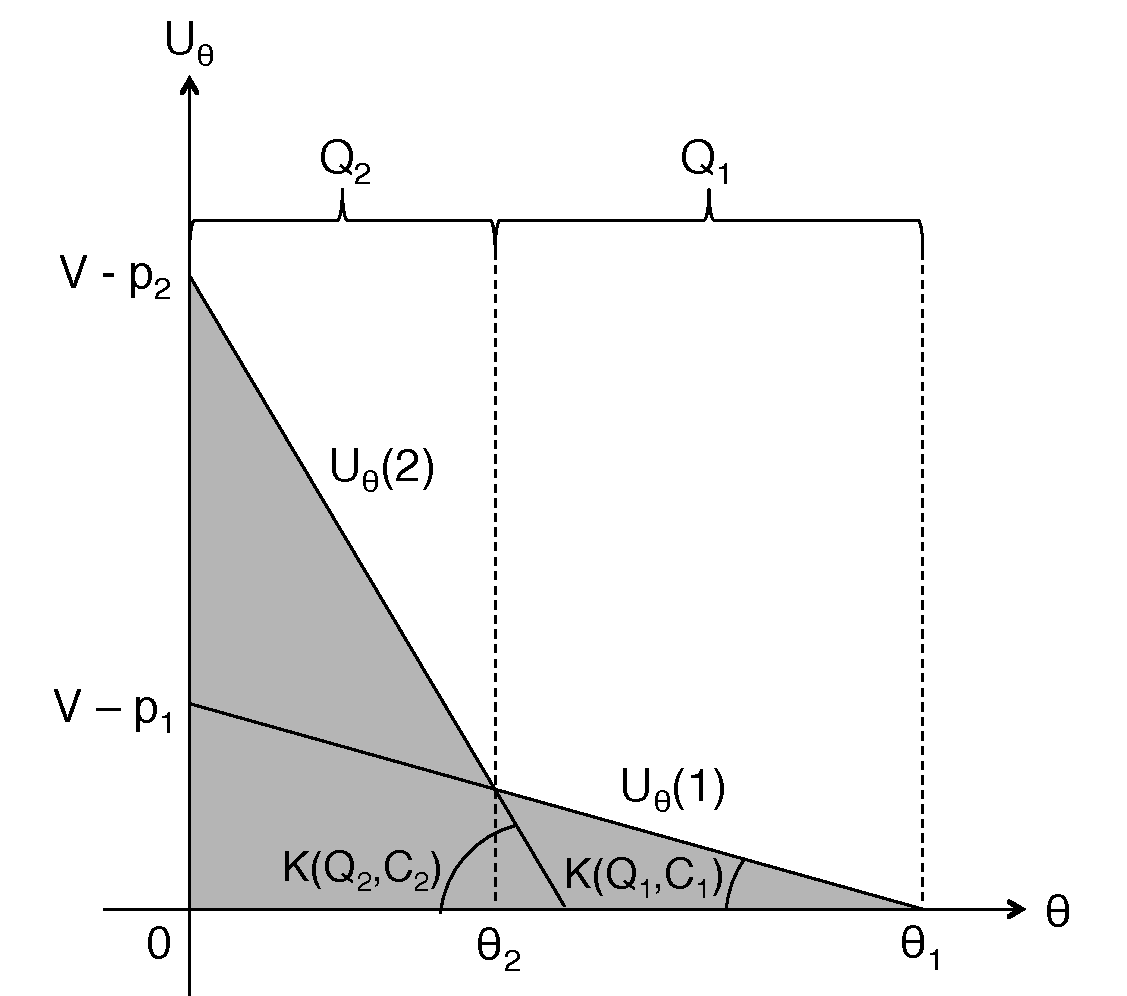
\includegraphics[width=8cm]{Figures/Equilibrium.pdf} 
\caption{\label{fig:equilibrium}Illustration of equilibrium in PMP.}
\end{figure}

Let $\theta_1$ be the $\theta$ of the user who is indifferent to joining the first service class or opting out of all the services, let $\theta_2$ be that of the user who is indifferent to joining the first service class or the second service class, and let $F(\theta)$ be the cumulative distribution function of $\theta$.
\begin{enumerate}
\item
Show that
\begin{subequations}
\begin{align*}
Q_1=&F(\theta_1)-F(\theta_2),\\
Q_2=&F(\theta_2),\\
V-p_1=&\theta_1 K(Q_1,C_1),\\
p_1-p_2=&\theta_2 (K(Q_2,C_2)-K(Q_1,C_1)).\\
\end{align*}
\end{subequations}

\item
Assume that $\theta$ is uniformly distributed, i.e., $F(\theta)=\theta$, and that the congestion function is defined as
$$K(Q,C)=\frac{Q}{C}.$$
Solve for $\theta_1$ and $\theta_2$ as functions of $V$, $p_1$, and $p_2$. 
\end{enumerate}

(Hint: Try $\frac{p_1-p_2}{V-p_1}$.)\\
 
(For details, see C. K. Chau, Q. Wang, and D. M. Chiu, ``On the Viability of Paris Metro Pricing for Communication and Service Networks," \emph{Proc. IEEE INFOCOM}, 2010.)\\

\item \emph{Two-Sided Pricing}

Taken from M. Chiang, \emph{Networked Life: 20 Questions and Answers}, Cambridge University Press, 2012.
\\ \\
Suppose an ISP charges a content provider (CP) the usage price $h_{CP}$ and flat price $g_{CP}$ and charges an end user (EU) the usage price $h_{EU}$ and flat price $g_{EU}$. For simplicity, we assume zero flat prices $\left(g_{CP}=g_{EU}=0\right)$. Let $\mu$ be the unit cost of provisioning capacity. The demand functions of the CP and EU, denoted as $D_{CP}$ and $D_{EU}$ respectively, are given as follows:\\
\begin{subequations}
\begin{align*}
D_{EU}(h_{EU})=&\left\{
\begin{array}{ll}
x_{EU,max}(1-\frac{h_{EU}}{h_{EU,max}})&\mbox{, if } 0\leq h_{EU}\leq h_{EU,max}\\
0,&\mbox{, if } h_{EU}>h_{EU,max}
\end{array}\right.\\
D_{CP}(h_{CP})=&\left\{
\begin{array}{ll}
x_{CP,max}(1-\frac{h_{CP}}{h_{CP,max}})&\mbox{, if } 0\leq h_{CP}\leq h_{CP,max}\\
0,&\mbox{, if } h_{CP}>h_{CP,max}.
\end{array}\right.\\
\end{align*}
\end{subequations}
The parameters are specified as follows:
\begin{subequations}
\begin{align*}
h_{CP,max}&=2.0\mu,\\
h_{EU,max}&=1.5\mu,\\
x_{CP,max}&=1.0,\\
x_{EU,max}&=2.0.\\
\end{align*}
\end{subequations}
The ISP maximizes its profit by solving the following maximization problem
\begin{equation}
\begin{array}{ll}
\mbox{maximize}	&(h_{CP}+h_{EU}-\mu)x\\
\mbox{subject to}	&x\leq \mbox{min}\{D_{CP}(h_{CP}),D_{EU}(h_{EU})\}\\
\mbox{variables} 	&x\geq 0, h_{CP}\geq 0, h_{EU}\geq 0.
\end{array}
\end{equation}

Find the optimal $x^\star, h_{CP}^\star, h_{EU}^\star$.\\

\item \emph{Monitoring Mobile Data Usage}

Many commercial mobile applications have been developed to help users keep track of their mobile data usage. Some examples include 3GWatchdog Pro (Android), DataWiz (iOS and Android), MyDataManager (Android), and Onavo Count (Android and iOS).
\begin{enumerate}
\item
Visit two or three app websites and list their features (e.g., showing usage by application, forecasting future usage, alerts when you approach your monthly data quota). Are there any significant differences between the apps? Can you identify any consistent differences between iOS and Android apps?
\item
What visual elements are used in the app designs? For instance, do the apps use bars or pie charts to represent usage? How are these displays different on different apps?
\item
Based on your answers to the above questions, try to design your own app for tracking mobile data usage. What screens would you implement? What features would you offer?
\end{enumerate}
\end{enumerate}

%[from Network 20Q?]
%
%Review questions. Multiple choice questions. 

% \section{20 Open Questions in SDP}\label{subsec:openQ}

%The term ``SDP'' encompasses all types of pricing for broadband data, from congestion-dependent pricing to two-sided pricing and even the intelligent (price-driven) offloading of traffic onto supplementary networks (e.g., 3G to WiFi). Some types of ``smart'' pricing plans include time, location, and/or congestion-dependent pricing; app-based pricing; smart offloading; two-sided pricing; and Paris metro pricing.
%
%All of these pricing plans aim to improve ISPs' traffic management by influencing consumer behavior. Yet designing a pricing plan for broadband data requires researchers to consider many factors--feasible algorithms to compute the prices offered and any other relevant variables, implementability of the pricing plan in a network, the pricing's effect on network operations, and--perhaps most important--acceptability of that pricing plan to end users, government regulators, and ISPs alike. These requirements and the inherent tradeoffs between them raise important questions that researchers are still trying to answer. For instance,
%\begin{itemize}
%\item
%Will users accept a dynamic pricing plan, in which prices change in real time depending on the network congestion? Is there a way to make such plans acceptable to users?
%\item
%Does app-based pricing (charging by the type of traffic, e.g., YouTube versus Netflix) violate network neutrality? Does it give larger, wealthier content providers undue advantage in subsidizing transmission of their content?
%\item
%Should ISPs charge for access to supplementary networks such as WiFi? If so, how much?
%\end{itemize}
%SDP research is driven by such questions. In our discussion, we attempt to highlight these types of tradeoffs and point to relevant research papers that address them. We first give an overview of  different pricing plans proposed by SDP research and deployed by ISPs, and then point to some emerging trends and open problems. For reasons of space, in this extended abstract we simply outline some of the topics and references that we plan to cover in the full book chapter. Relevant references may be found in our survey paper on broadband data pricing \cite{computing-survey}.
%
\section{Supplementary Materials} \label{subsec:supp}

As a part of the supplementary reading materials for the chapter, students are encouraged to refer to the following materials:
\begin{itemize}
\item Slides on Time-dependent Usage-based pricing engineering (TUBE) and shared data plans.
\item Chapter 12 from M. Chiang's book\\ (http://www.amazon.com/Networked-Life-20-Questions-Answers/dp/1107024943) \cite{chiang2012networked}.
\item Lecture notes, slides and homework questions on SDP from ELE 381\\ (http://scenic.princeton.edu/network20q/).
\item Course videos on SDP (Coursera material available at https://www.coursera.org/course/friendsmoneybytes; videos available at http://www.youtube.com/watch?v=MMl\_fZypX0w, \\ http://www.youtube.com/watch?v=N2oM0ISs0nY, http://www.youtube.com/watch?v=v\_uHP4SNKGo, http://www.youtube.com/watch?v=21KlcErIiHc) \cite{coursera}.
\item Demo videos related to the DataMi project (http://scenic.princeton.edu/datami/) \cite{datami}. 
\item Free DataWiz iPhone and Android app for usage monitoring \\ (download links at http://scenic.princeton.edu/datawiz/) \cite{datawiz}.
\item Research papers, surveys, and white papers from SDP workshops\\ (available at http://scenic.princeton.edu/SDP2012/program.html) \cite{SDPForum}.
% \item Relevant chapter pre-prints from the upcoming Smart Data Pricing (SDP) Book, edited by the authors for John Wiley \& Sons. 
\end{itemize}

\appendix

\section{Data Plans around the World}\label{Dataplans}

In most countries, the dominant forms of mobile data pricing are still usage-based or tiered. However, the actual cost of mobile data can vary greatly from country to country, depending on such factors as the country's network infrastructure, market competition, and population density. One common distinction is between pre- and postpaid plans.\footnote{Prepaid plans are those in which a consumer pays for his/her data usage beforehand, while for postpaid plans, a consumer is billed for his/her monthly usage at the end of the billing cycle.} Castells et al. \cite{castells2007mobile} found a strong correlation between the availability of prepaid plans for voice calls and adoption rates of mobile telephone subscribers, which is corroborated by Hauge et al. \cite{hauge2009whose}.  In this Appendix, we provide an overview of prepaid and postpaid plan adoption in different parts of the world and its relationship to consumer market demographics.

\begin{figure}
\centering
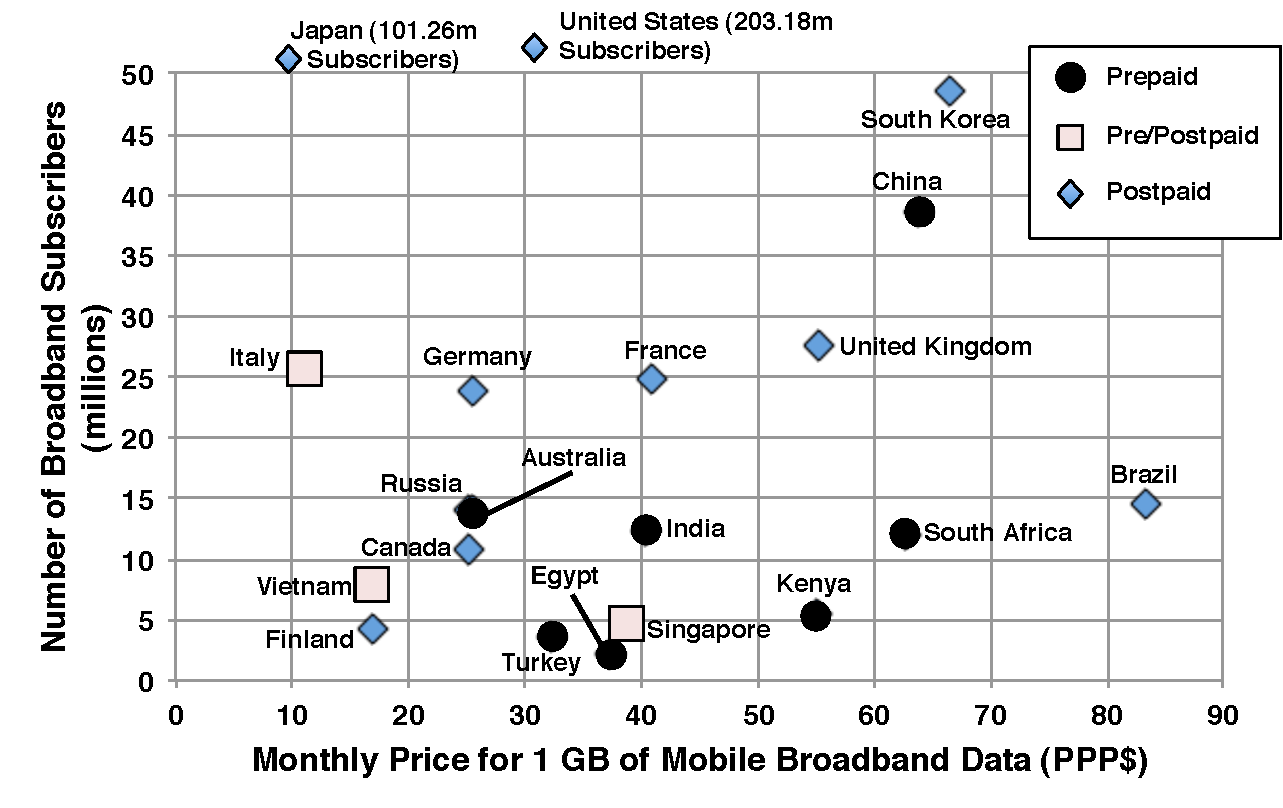
\includegraphics[width=0.75\textwidth]{Figures/World.pdf}
\caption{Prepaid and postpaid mobile broadband data plans around the world (data from 2011).  Data were taken from operator websites as well as \cite{chinamobile,SAfrica,cia,kenyatotal,egypttotal,singapore,itu,italy,india,docomo,oecd,chinatotal,russiatotal,braziltotal,korea,vietnamtotal,worldbank}.}
\label{fig:world}
\end{figure}

\begin{figure}
\centering
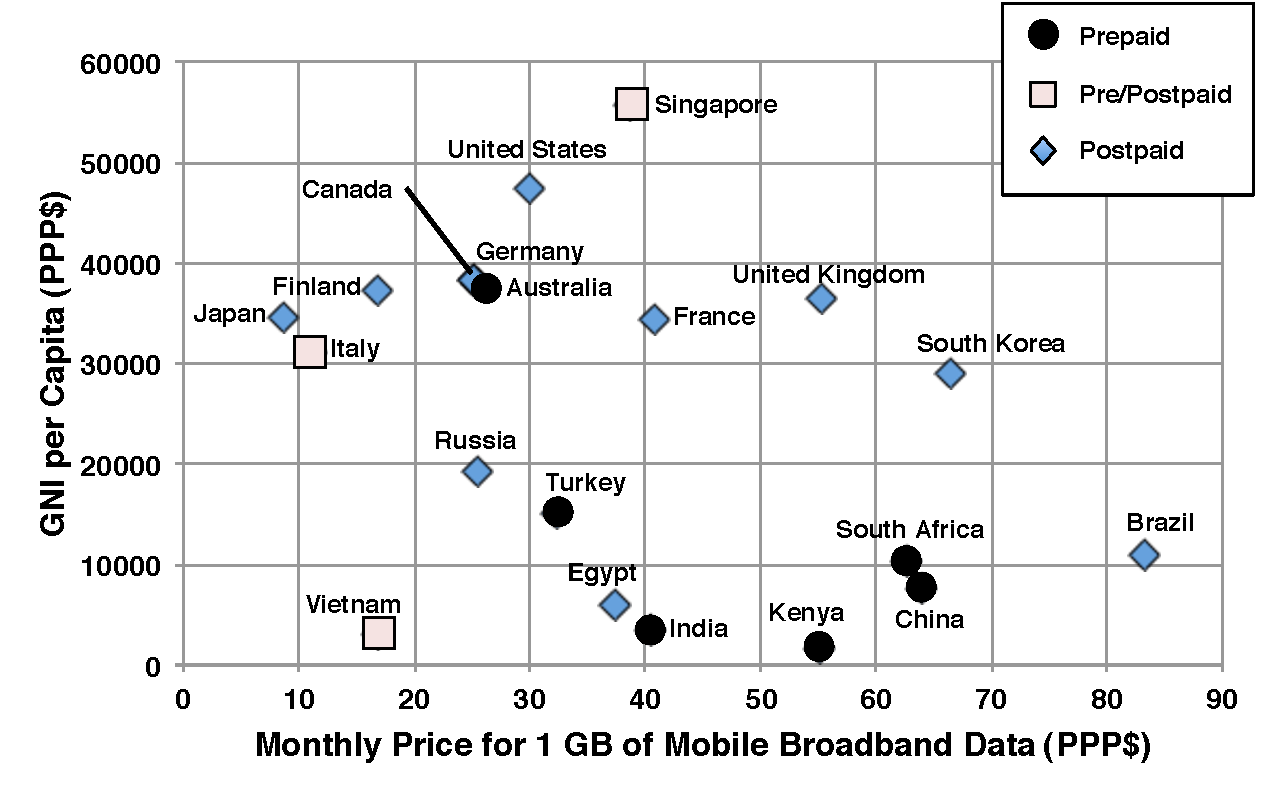
\includegraphics[width=0.75\textwidth]{Figures/GNI.pdf}
\caption{GNI per capita vs. monthly cost of 1GB of mobile data (data sources as in Figure \ref{fig:world}).}
\label{fig:gni}
\end{figure}

\begin{figure}
\centering
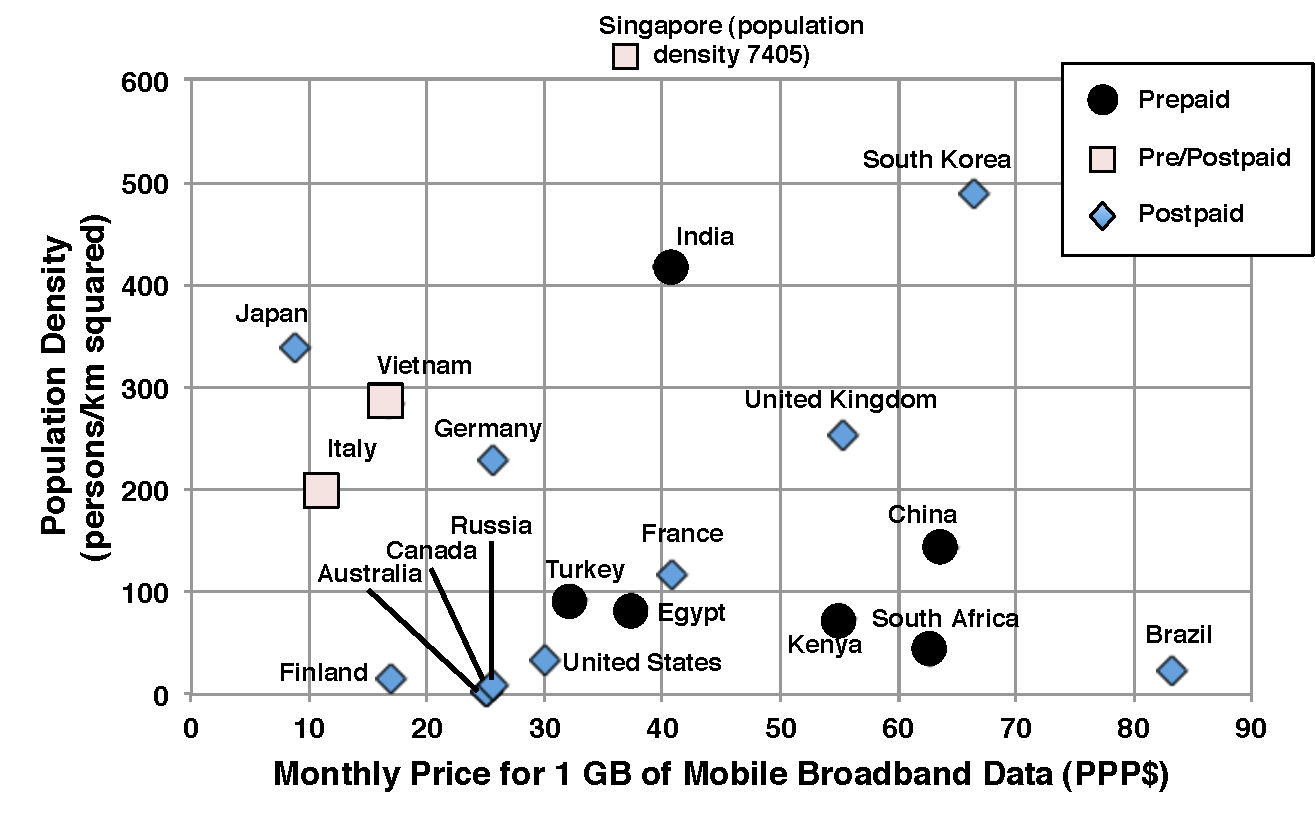
\includegraphics[width=0.75\textwidth]{Figures/Density_PPP.pdf}
\caption{Population density vs. monthly cost of 1GB of mobile data (data sources as in Figure \ref{fig:world}).}
\label{fig:density}
\end{figure}

Figure \ref{fig:world} shows whether prepaid or postpaid plans are the dominant form of data plans in several countries of the world, as of 2011. To determine this data, we examined the standard mobile subscriptions for the largest mobile operator in each country and plotted the monthly cost (in \$ after accounting for purchasing power parity) of 1GB of data usage.  We note that the data plans in different countries have different broadband caps, which are not reflected in the graph, but may be found in \cite{itu}. The cost of 1GB of data/month has been plotted against the number of mobile broadband subscribers in each country; we observe that there is a large variation in cost. Additionally, we see that the countries of Africa (e.g., Kenya, South Africa), the Middle East (e.g., Turkey, Egypt), India and China tend to prefer prepaid plans, while postpaid plans dominate in Europe and the Americas. There is a weakly positive correlation between the price for mobile data and the number of broadband subscribers in the country.

Figure \ref{fig:gni} more explicitly shows the correlation between prepaid mobile broadband data plans and lower per capita gross national incomes (GNI): we see that countries with a lower GNI per capita tend to have prepaid plans as the dominant subscription mode, with the exception of Australia.  Moreover, two of the three countries offering both pre- and postpaid plans (Italy and Vietnam) have GNI per capita below the wealthiest 9 countries. Wealthier countries tend to have lower prices for mobile data, even accounting for purchasing power parity. In lower-GNI countries, it is possible that only a wealthy subset who can afford higher prices generally purchase mobile data plans; another explanation is that these countries have lower investment costs due to their relative wealth.

Infrastructure development is also related to population density: in denser countries, networks need to cover a smaller geographical area to reach the same number of people, resulting in lower investment costs. In the rural United States, small carriers often cite wireline backhaul over long distances as a major source of wireless network costs \cite{neca}. Figure \ref{fig:density} shows a negative correlation between population density and the price for 1GB of mobile data, consistent with our hypothesis that denser countries have lower infrastructure costs. Prepaid data plans are somewhat more popular in less dense countries, with India a notable exception: 83\% of countries with prepaid plans have lower population density than 36\% of countries with high population density and postpaid data plans. These countries also tended to have lower GNIs, which along with their population density suggest that their network infrastructure is less comprehensive than that of denser, wealthier countries.

% Within the U.S., prepaid data plans have gained popularity due to their lower, shorter-term financial commitment and relative simplicity compared to postpaid usage-based pricing plans with data caps.  Moreover, operators are offering more attractive prepaid devices with data-centric plans that appeal to young, price-sensitive users \cite{pcworld}.

%\section{Coping with Usage-based Pricing}
%
%While usage-based pricing is one of the simplest pricing plans, besides charging flat fees for unlimited usage, a major limitation to usage pricing is that many people do not understand how much data their applications use. Thus, even tiered data plans with monthly caps can be hard for them to manage. Several user apps have been developed to 

%\section{Our Qualifications}\label{sec:qualf}
%
%\subsection{Teaching Experience}
%
%M. Chiang has recently started a new undergraduate course (ELE 381) called ``Networks: Friends, Money, and Bytes,'' which was offered in the fall of 2011 and again in the fall of 2012 at Princeton University\footnote{More details may be found on the course website, http://scenic.princeton.edu/network20q.}. The graduate level version of the course was offered in the spring of 2012, covering more in-depth material on social networks, network economics, and network management. Beginning this fall, a version of the undergraduate course is also offered on Coursera, where it has over 40,000 enrolled students. Of particular relevance to this book chapter is the week spent on SDP; one lecture is spent entirely on dynamic time-dependent pricing, while another covers other forms of SDP, including usage-based and two-sided pricing. S. Ha, C. Joe-Wong, and S. Sen have given guest lectures on dynamic time-dependent pricing in both the undergraduate and graduate versions of this course.
%
%The Princeton version of Networks: Friends, Money, and Bytes follows a flipped classroom model \cite{flipped}, in which students watch lecture videos and read the lecture notes outside of the class, while class time is reserved for problem solving sessions, demos, and other interactive activities. Thus, two lecture videos on SDP have already been recorded and will be made publicly available on YouTube later this year. These and other course materials, including homework questions and lecture notes, can be made available as part of the Sigcomm e-book chapter for students. The course's accompanying textbook, also authored by M. Chiang, has been recently published by Cambridge University Press; it gives more background on the course topics and is organized around the lecture material \cite{chiang2012networked}.  The book's chapter on dynamic time-dependent pricing is available online\footnote{URL: http://www.princeton.edu/$\sim$cjoe/Ch12\_Network20Q.pdf}.  In addition to classroom teaching, S. Sen and M. Chiang have offered tutorials on SDP to the members of National Exchange Carrier Association (NECA) in Chicago (2011) and Seattle (2012), and will be hosting a tutorial at IEEE Globecom in December 2012. 
%
%\subsection{Research Experience}
%
%Our understanding of SDP from a teaching perspective is informed by the authors' long-standing experience and knowledge of network economics. We have published in several prestigious journal and conferences, including IEEE/ACM Transactions on Networking (M. Chiang and S. Sen), IEEE JSAC (M. Chiang, S. Ha, C. Joe-Wong, and S. Sen), ACM SIGCOMM Computer Communications Review (M. Chiang and S. Sen), SIGCOMM (S. Ha, S. Sen, C. Joe-Wong, and M. Chiang), IEEE INFOCOM (M. Chiang, S. Ha, C. Joe-Wong, and S. Sen), and IEEE ICDCS (M. Chiang, S. Ha, and C. Joe-Wong). Our major publications on SDP specifically are cited in the references and in the discussion below. C. Joe-Wong, S. Sen and M. Chiang also received the Best Paper Award at IEEE INFOCOM 2012 for their work on fairness-efficiency tradeoffs in network resource allocation \cite{joe2012multi}.
%
%Our research project, DataMi \cite{datami}, encompasses time-dependent pricing, intelligent throttling, and smart offloading onto supplementary networks. In particular, we have conducted the first consumer trial of time-dependent pricing for mobile data, the results of which were published in ACM SIGCOMM 2012 paper \cite{ha2012tube}; a preliminary version of this work was published in IEEE ICDCS 2011 \cite{Carlee}. We have also showcased demos of this time-dependent pricing system, called TUBE (Time-dependent Usage-based Broadband price Engineering), which were featured at both IEEE INFOCOM 2012 and ACM MobiSys 2012 \cite{ha2012demo}; demo videos have been made available online on our YouTube channel at http://www.youtube.com/user/princetonedge. We have also published an extension of our time-dependent pricing model to electricity markets, which was published in JSAC in July 2012 \cite{joe2012optimized}, and have worked on the economics of shared data plans \cite{WITS} and pricing in heterogeneous networks \cite{wifi-3g-infocom}. Several slide presentations of our work are also available online\footnote{Time-dependent pricing slides based on \cite{ha2012tube} are available at http://www.princeton.edu/$\sim$sangtaeh/TUBE\_SIGCOMM\_Slides.pdf; slides on pricing of heterogeneous networks, based on \cite{wifi-3g-infocom}, are available at http://www.princeton.edu/$\sim$cjoe/Offloading\_GSS\_Slides.pdf.} and will be included as part of the supplementary material for this Sigcomm e-book chapter.
%
%In addition to technical research papers, all four co-authors have written a position paper on SDP that will appear in IEEE Communications Magazine later this year \cite{comm-mag}. The paper, which is accessible to the general networking community as well as graduate students in the field, argues that in order to manage the growth in demand for data, future broadband data plans will need to utilize prices to incentivize changes in user behavior. It includes an overview of data plans currently offered around the world, as well as discussions of regulatory and net neutrality perspectives on different forms of SDP and a survey of relevant literature on time-dependent pricing. A more extensive literature survey, including the pricing of electricity and road networks, has been submitted to ACM Computing Surveys and received positive reviews; it is currently under submission. A draft has been made available online \cite{computing-survey}.
%
%\subsection{Industry Experience}
%
%We have supplemented our research experience with extensive interactions with industry and government bodies. In particular, our TUBE project on time-dependent pricing was a finalist in the 2011 Vodafone Wireless Innovation Competition, which aimed to reward projects that used novel wireless technologies to make a global impact. We also presented our work on TUBE at the NECA (National Exchange Carrier Association) Expo in 2011, and as a result of that collaboration are beginning a trial of TUBE with an Alaskan operator, MTA \cite{datami}. TUBE was also presented at the 2011 Keller Center Innovation Forum and the 2011 Princeton Innovation Forum, which showcased technologies from Princeton professors that showed market potential. More academic venues in which we presented TUBE include invited talks at Alcatel-Lucent Bell Labs, Korea Telecom, and the Workshop on Internet Topology Economics (WITE) hosted by Georgia Tech (all in 2012).
%
%In July 2012, S. Sen and M. Chiang organized and hosted the first SDP Forum, in which numerous leaders from academia and industry gave talks and participated in panel discussions on SDP's future role, both in terms of research and broadband markets. The slides presented are available online at http://scenic.princeton.edu/SDP2012. Forum participants included representatives from Alcatel-Lucent, AT\&T Labs, Cisco, Comcast, Korea Telecom, Microsoft Research and Qualcomm. We are in the process of editing a book documenting the proceedings and invited contributions of chapters for release in early 2013 by John Wiley \& Sons. A proposal for the second SDP forum is under consideration for a workshop at IEEE INFOCOM 2013 in Turin, Italy.


%\bibliographystyle{ieeetr}

% Define style for bibtex bibliography
\bibliographystyle{../acm}
\bibliography{Citations}

%\section*{Author Biographies}

%{\bf Soumya Sen} received the B.E. (Hons.) in Electronics and Instrumentation Engineering from BITS-Pilani, India, in 2005, and both the M.S. and Ph.D. in Electrical and Systems Engineering from the University of Pennsylvania in 2008 and 2011, respectively, and did his postdoctoral research at the Princeton University. He is currently an Assistant Professor in the Department of Information \& Decision Sciences at the Carlson School of Management of the University of Minnesota. He is a co-organizer of the Smart Data Pricing (SDP) Forum, which promotes industry-academic interaction on broadband pricing research. His research interests are in Internet economics, communication systems, social networks, and network security. He has published several research articles in these areas and his work on broadband pricing was a f\hspace{0.01mm}inalist at the 2011 Vodafone Wireless Innovation project. He won the Best Paper Award at IEEE INFOCOM 2012.\\

%\noindent {\bf Carlee Joe-Wong}
%is a graduate student at Princeton University's Program in Applied and Computational Mathematics.  She received the A.B. degree (magna cum laude) in mathematics from Princeton University in 2011.  Currently, she is Director of Advanced Research at DataMi, a startup she co-founded in 2012 that aims to make mobile networks more efficient through better incentive and capacity management. Her research interests include network economics and optimal control theory. She won the Best Paper Award at IEEE INFOCOM 2012 for her work on the fairness of multi-resource allocations.  In 2011, she received the National Defense Science and Engineering Graduate Fellowship. \\

%\noindent {\bf Sangtae Ha} is the CTO and VP Engineering at DataMi. He received his Ph.D. in Computer Science from North Carolina State University in 2009. During his Ph.D. study, he co-authored CUBIC, a new mechanism for TCP congestion control, and was the primary engineer pushing it into Linux 2.6.18. CUBIC has been the default TCP congestion control algorithm in Linux since 2006 and is currently used by more than 40\% of Internet servers around the world as well as several hundred million Android/Linux devices.  After completing his Ph.D., he co-founded the Princeton EDGE Lab (http://scenic.princeton.edu) as its first Associate Director in 2009 and led its research team as an Associate Research Scholar at Princeton University from 2010 to 2013. In particular, he led the DataMi (http://www.datami.com) project team, which develops Smart Data Pricing (SDP) solutions to help Internet Service Providers (ISPs) meet the increasingly untenable demand for mobile data.  He is a co-founder of DataMi Inc. and a technical consultant to a few startups. He is an IEEE Senior Member and was a general co-chair of the Smart Data Pricing workshop in INFOCOM 2013. \\

%\noindent {\bf Mung Chiang} is the Arthur LeGrand Doty Professor of Electrical Engineering at Princeton University, and an affiliated faculty in Applied and Computational Mathematics, and in Computer Science. He received his B.S. (Hons.), M.S., and Ph.D. degrees from Stanford University in 1999, 2000, and 2003, respectively, and was an Assistant Professor 2003-2008, an Associate Professor 2008-2011, and a Professor 2011-2013 at Princeton University. His research on networking received the Alan T. Waterman Award (2013), IEEE Kiyo Tomiyasu Award (2012), a U.S. Presidential Early Career Award for Scientists and Engineers (2008), several young investigator awards, and a few paper awards including the IEEE INFOCOM Best Paper Award (2012). A recipient of the Technology Review TR35 Award (2007), his inventions have resulted in a few technology transfers and commercializations. In 2009, he founded the Princeton EDGE Lab, supported in part by an industry consortium, which aims at bridging the theory-practice divide in networking. He served as an IEEE Communications Society Distinguished Lecturer in 2012-2013, chaired the founding steering committee of the new IEEE Transactions on Network Science and Engineering, and co-chaired the 2012 US NITRD special workshop on complex engineered networks. He created a new undergraduate course: �Networks:  Friends, Money, and Bytes� that lead to an open online offering and a flipped classroom at Princeton. The corresponding textbook: �Networked Life: 20 Questions and Answers,'' provided the Integrated and Individualized BookApp (IIB) format, and received the PROSE Award in Engineering and Technology (2013) from the Association of American Publishers. In 2013, he initiated the online learning platform, ``3 Nights and Done.'' 

\end{document}